\chapter{Results}
\label{chap:results}
This chapter will introduce the results of the data analysis. I will touch on some topics for discussion for some of the results, however most of the discussion will take place in chapter \ref{chap:discussion}. This chapter will start by describing the demographics and background of the main sample. Further, I will present the results from the univariate analysis that assess the security awareness of the respondents. Next I present my findings from the bivariate analysis, and lastly present and compare the results from my control group sample. 

\section{Demographics}

The following section will describe the demographics of my samples, as well as compare relevant groups to each other and the Norwegian national population. Out of the total of 222 people who answered, one person did not want to specify any demographic data. 

\subsection{Age}
The age distribution of my sample. None of the respondents reported being under 20 years old. 33 (14.9\%) of the respondents answered being between 20 and 29 years old and a whole 102 (45.9\%) responded that they are between 30 and 39 years old, which is the largest age group of our sample. Further, 56 (25.2\%) people answered being between 40 and 49 years old, which is the second largest age group. Lastly, 24 (10.8\%) of my sample is between 50 and 59 years old and 6 (2.7\%) people being 60 or older. 
\begin{figure}[!h]
    \centering
    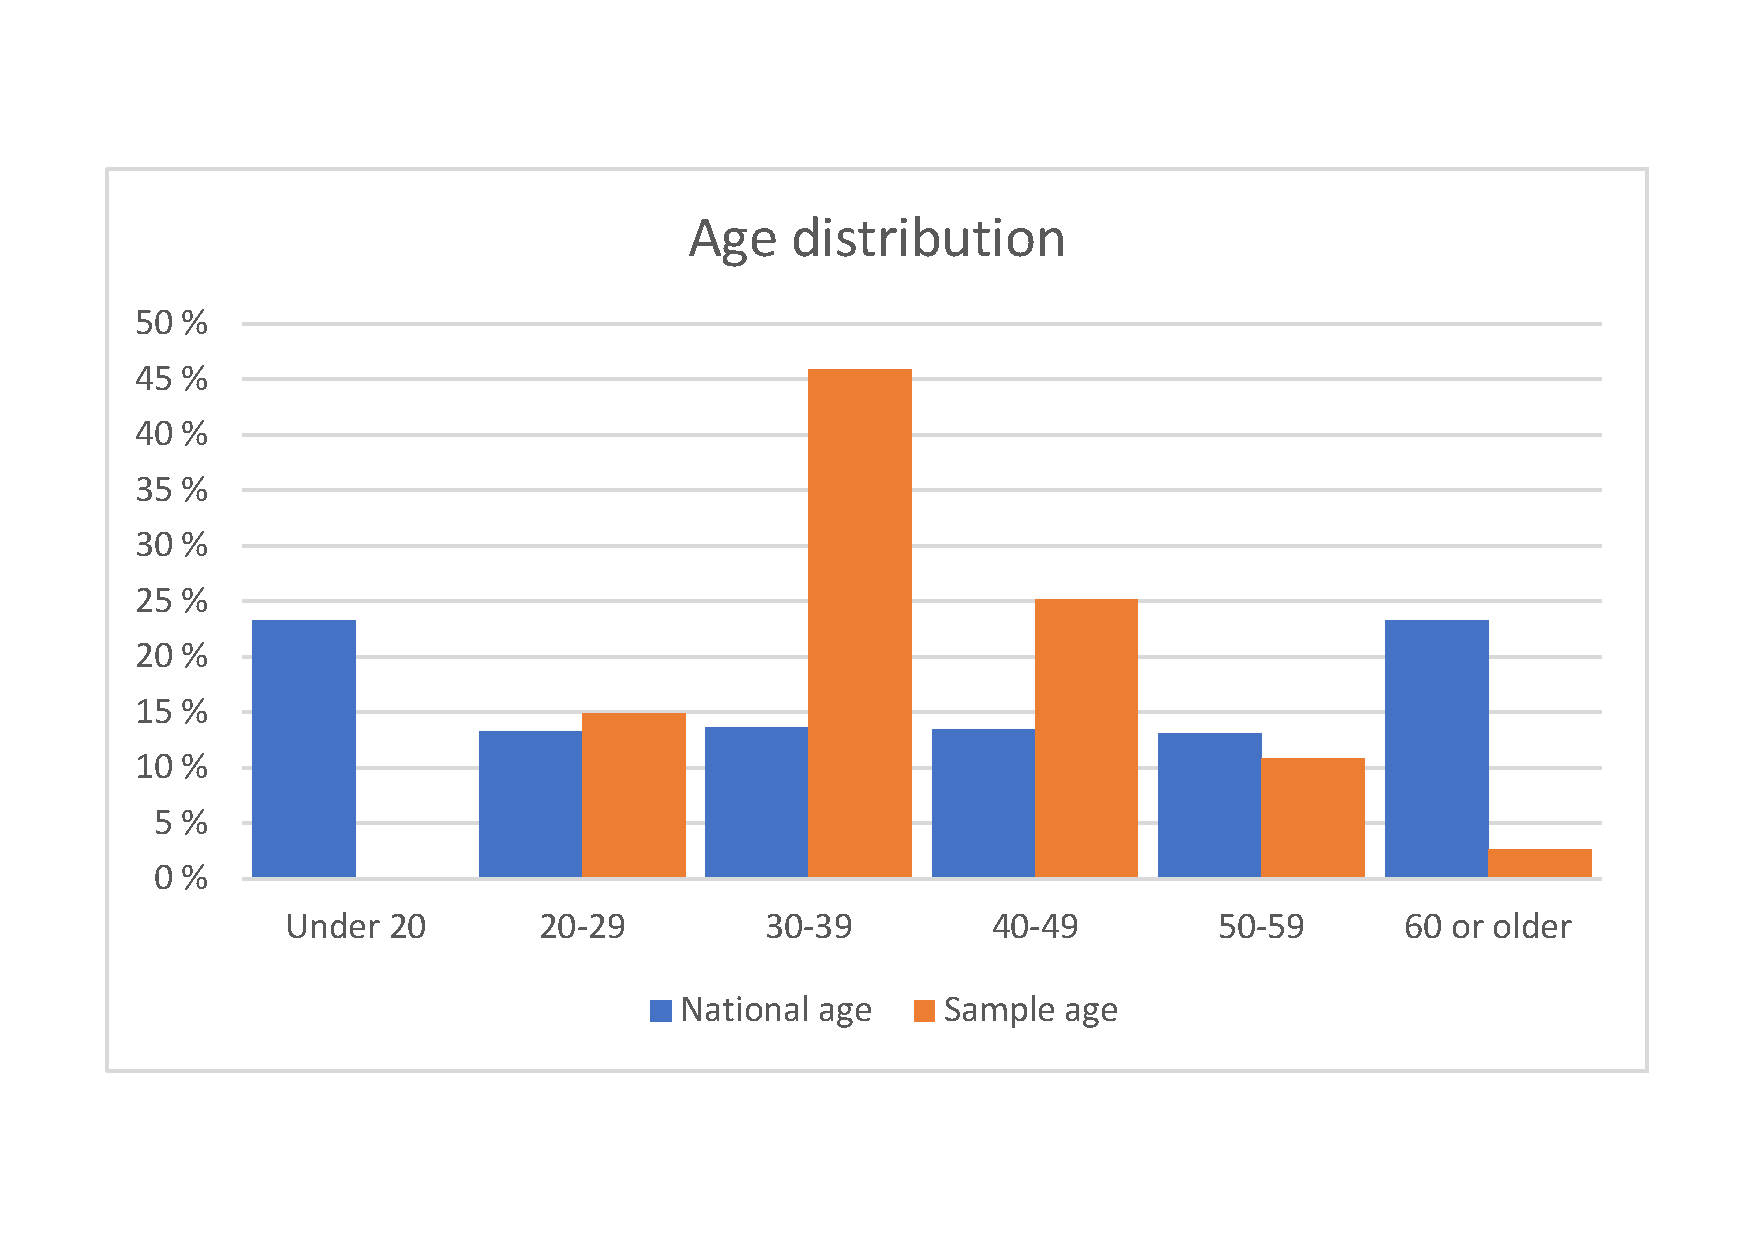
\includegraphics[scale=0.45]{figures/diagrams/age_ssb.pdf}
    \caption{Age distribution}
    \label{fig:age}
\end{figure}

As we can see from figure \ref{fig:age}, we have a fairly middle-aged sample compared to the national population, which has a sizeable difference in younger and older people compared to my sample. 

Since the number of respondents being 60 or older in my sample only comprise 6 respondents, I will merge that category with 50-59 years going forward, resulting in a single category of 50 or older. This will result in the category comprising 30 respondents, which should be the minimum for further analysis between the groups. 

\subsection{Gender}
\label{subsec:gender}
The gender distribution of my main sample is all men. There were also one respondent who did not want to specify, however there are no women in my sample. This makes it impossible to use in further analysis other than for sample description. This is obviously a huge deviation from the national average of approximately 50\% of each gender. 


\subsection{Highest completed education level}
None of the respondents answered that they had only primary school education or no education, and only one person did not want to specify education level. 48 people (21.6\%) answered that they has completed high school, while 55 of the respondents (24.8\%) has completed vocational college. 76 people (34.2\%) has completed at least four year university or college, and 42 (18.9\%) has completed university or college for longer than four years. 
\begin{figure}[!h]
    \centering
    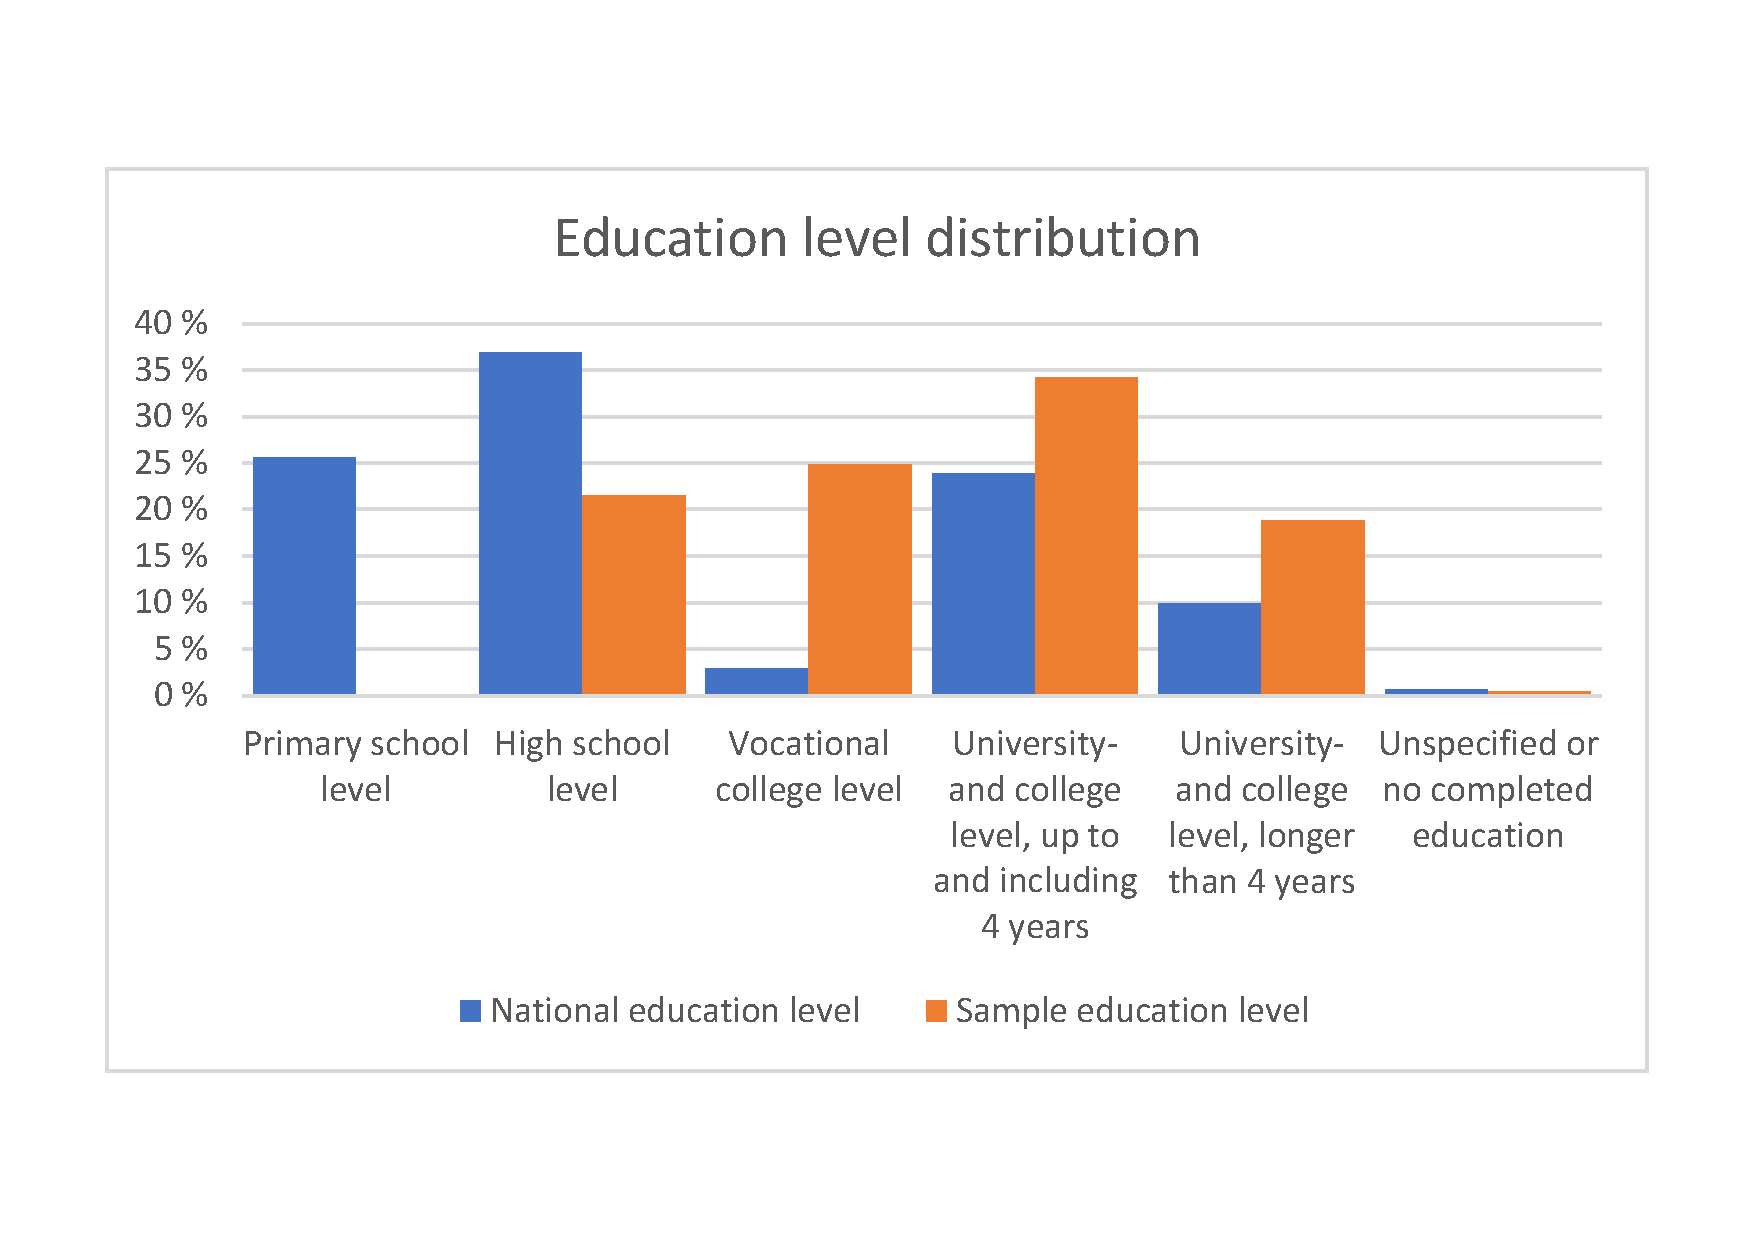
\includegraphics[scale=0.45]{figures/diagrams/education_ssb.pdf}
    \caption{Highest completed education level}
    \label{fig:education}
\end{figure}

From figure \ref{fig:education} above we can see that my sample contain a higher share of people with higher education. The most interesting fact is that the data shows a huge difference when it comes to people reporting to having a vocational education. 

\subsection{County}
There were two people who did not want to specify which county they lived in. The sample distribution in figure \ref{fig:county} below shows that it is very close to the national distribution. The only significant outlier is that my sample has a bit more people from Rogaland (14\%), compared to the national level (9\%).
\begin{figure}[!h]
    \centering
    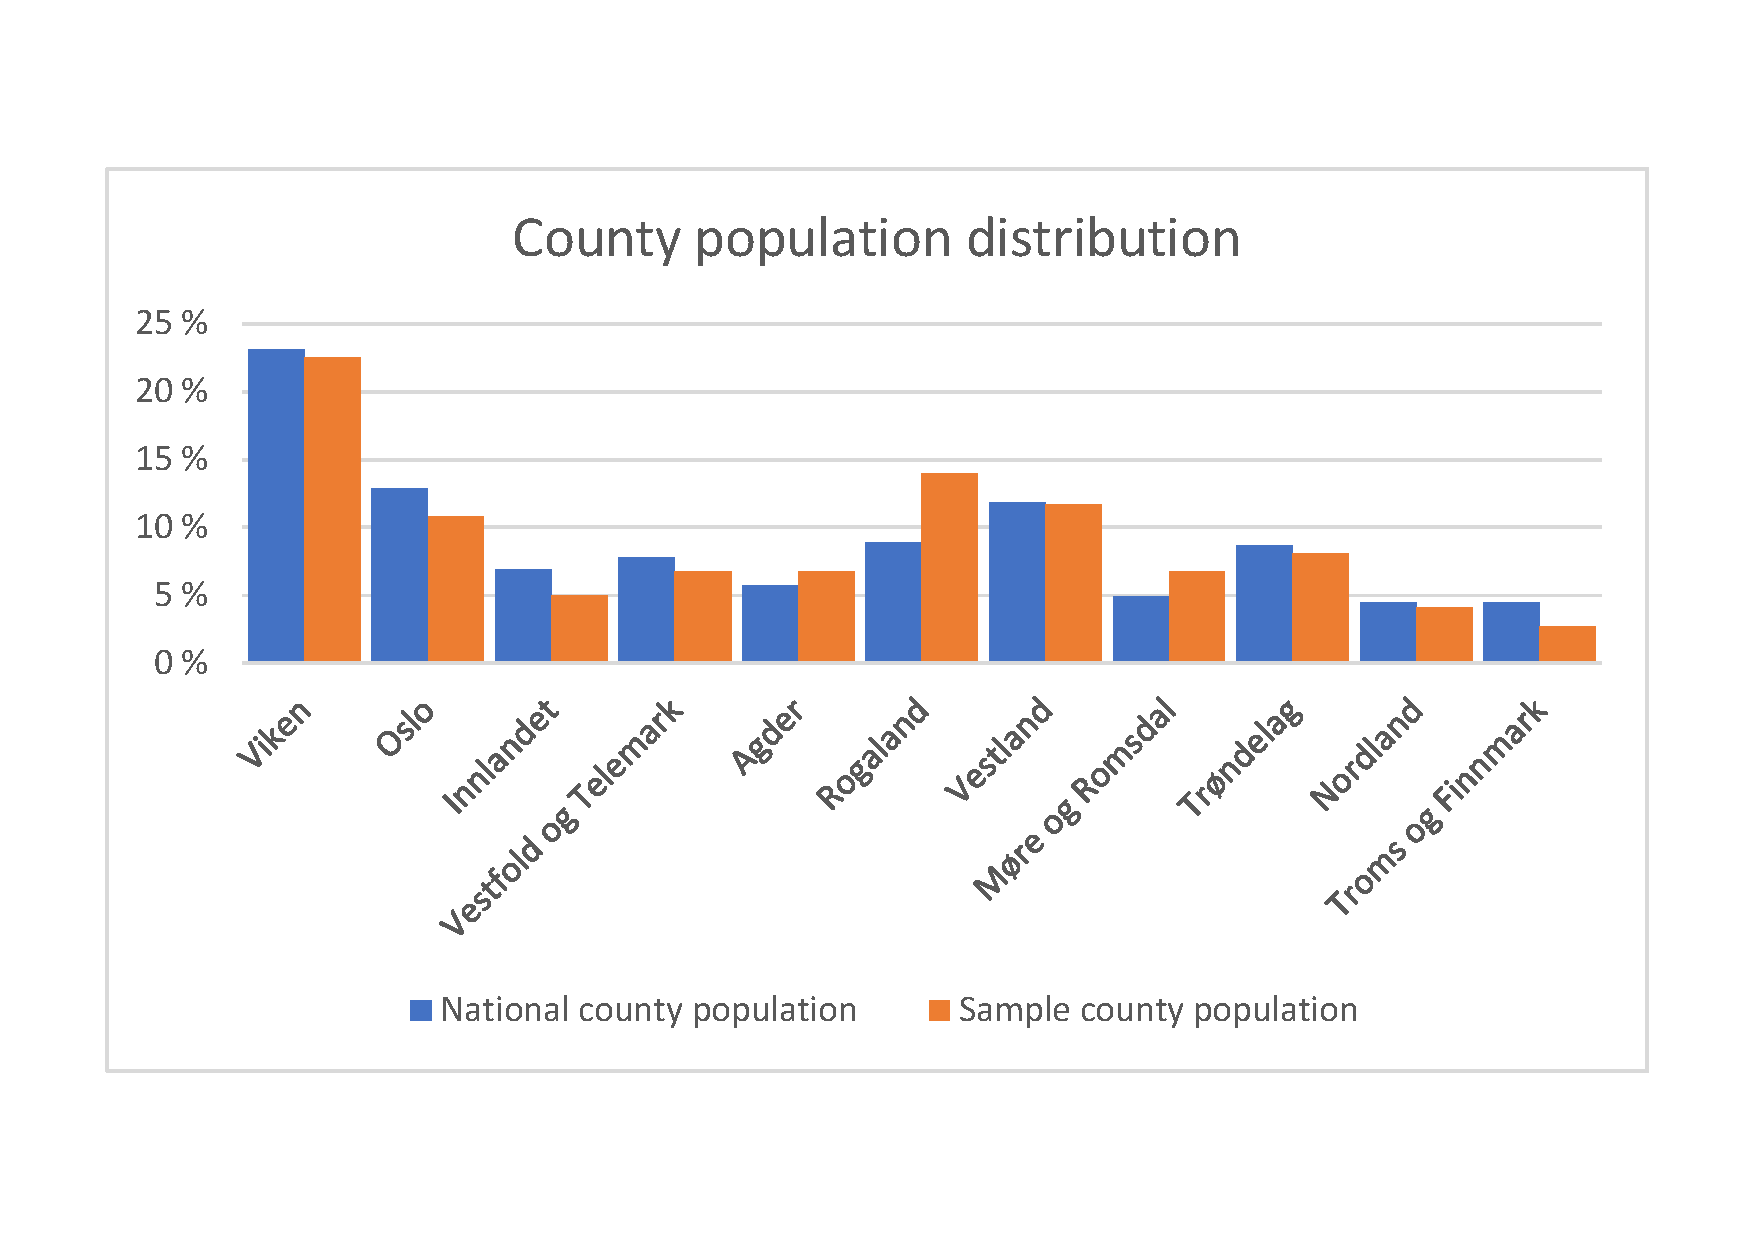
\includegraphics[scale=0.45]{figures/diagrams/county_ssb.pdf}
    \caption{County population distribution}
    \label{fig:county}
\end{figure}

It should be mentioned that most of the categories from my sample has less than 30 answers, which might impact the comparability of the numbers. For example, Troms og Finnmark only has 6 respondents in my sample, and Nordland has 9 respondents. At the other end of the spectrum lies Viken with 50 respondents and Rogaland with 31 respondents. 

\section{Background}

\subsection{How smart are the homes?}
In order to investigate how invested people are in the smart home ecosystem, I chose to include a question that aimed to assess which smart device types the respondents owns. In table \ref{tab:how_smart_N} below is an overview of the number of respondents that answered this question. 

\begin{table}[!h]
\centering
\begin{tabular}{|l|c|c|c|c|c|c|}
\hline
\multicolumn{7}{|c|}{{\color[HTML]{010205} \textbf{Case summary}}}                                                                                                                                                                                                                                                                                                              \\ \hline
{\color[HTML]{264A60} }                                      & \multicolumn{6}{c|}{{\color[HTML]{264A60} Cases}}                                                                                                                                                                                                                                                                \\ \cline{2-7} 
{\color[HTML]{264A60} }                                      & \multicolumn{2}{c|}{{\color[HTML]{264A60} Valid}}                                                    & \multicolumn{2}{c|}{{\color[HTML]{264A60} Missing}}                                               & \multicolumn{2}{c|}{{\color[HTML]{264A60} Total}}                                                     \\ \cline{2-7} 
\multirow{-3}{*}{{\color[HTML]{264A60} }}                    & {\color[HTML]{264A60} N}                        & {\color[HTML]{264A60} Percent}                     & {\color[HTML]{264A60} N}                      & {\color[HTML]{264A60} Percent}                    & {\color[HTML]{264A60} N}                        & {\color[HTML]{264A60} Percent}                      \\ \hline
\cellcolor[HTML]{E0E0E0}{\color[HTML]{264A60} Smart devices} & \multicolumn{1}{r|}{{\color[HTML]{010205} 219}} & \multicolumn{1}{r|}{{\color[HTML]{010205} 98.6\%}} & \multicolumn{1}{r|}{{\color[HTML]{010205} 3}} & \multicolumn{1}{r|}{{\color[HTML]{010205} 1.4\%}} & \multicolumn{1}{r|}{{\color[HTML]{010205} 222}} & \multicolumn{1}{r|}{{\color[HTML]{010205} 100.0\%}} \\ \hline
\end{tabular}
\caption{Number of people who specified what smart device types they own}
\label{tab:how_smart_N}
\end{table}

Out of the three that did not answer, two of them specified in free text that they used a KNX system with control of heating, lighting, and ventilation, as well as motion sensors among other things. Multiple people who answered, also specified in free text that they used a KNX system, and many others specified that they had a smart home with basically ``everything''. One respondent answered that they had no smart devices. The table below shows the frequency of which types of smart devices the respondents owned. 
\begin{table}[!h]
\centering
\begin{tabular}{|l|l|r|r|r|}
\hline
\multicolumn{5}{|c|}{\textbf{Smart device types frequencies}}                                                                                                                                                                                                                                                                           \\ \hline
\multicolumn{2}{|l|}{}                                                                                                                           & \multicolumn{2}{c|}{{\color[HTML]{264A60} Responses}}                                               & \multicolumn{1}{c|}{{\color[HTML]{264A60} }}                                   \\ \cline{3-4}
\multicolumn{2}{|l|}{\multirow{-2}{*}{}}                                                                                                         & \multicolumn{1}{c|}{{\color[HTML]{264A60} N}} & \multicolumn{1}{c|}{{\color[HTML]{264A60} Percent}} & \multicolumn{1}{c|}{\multirow{-2}{*}{{\color[HTML]{264A60} Percent of Cases}}} \\ \hline
\cellcolor[HTML]{E0E0E0}{\color[HTML]{000000} }                                 & \cellcolor[HTML]{E0E0E0}{\color[HTML]{264A60} Voice assistant} & {\color[HTML]{010205} 155}                    & {\color[HTML]{010205} 6.7\%}                        & {\color[HTML]{010205} 70.8\%}                                                  \\ \cline{2-5} 
\cellcolor[HTML]{E0E0E0}{\color[HTML]{000000} }                                 & \cellcolor[HTML]{E0E0E0}{\color[HTML]{264A60} Speaker}         & {\color[HTML]{010205} 158}                    & {\color[HTML]{010205} 6.8\%}                        & {\color[HTML]{010205} 72.1\%}                                                  \\ \cline{2-5} 
\cellcolor[HTML]{E0E0E0}{\color[HTML]{000000} }                                 & \cellcolor[HTML]{E0E0E0}{\color[HTML]{264A60} Robot vaccum}    & {\color[HTML]{010205} 123}                    & {\color[HTML]{010205} 5.3\%}                        & {\color[HTML]{010205} 56.2\%}                                                  \\ \cline{2-5} 
\cellcolor[HTML]{E0E0E0}{\color[HTML]{000000} }                                 & \cellcolor[HTML]{E0E0E0}{\color[HTML]{264A60} Smart hub}       & {\color[HTML]{010205} 169}                    & {\color[HTML]{010205} 7.3\%}                        & {\color[HTML]{010205} 77.2\%}                                                  \\ \cline{2-5} 
\cellcolor[HTML]{E0E0E0}{\color[HTML]{000000} }                                 & \cellcolor[HTML]{E0E0E0}{\color[HTML]{264A60} Smart TV}        & {\color[HTML]{010205} 185}                    & {\color[HTML]{010205} 8.0\%}                        & {\color[HTML]{010205} 84.5\%}                                                  \\ \cline{2-5} 
\cellcolor[HTML]{E0E0E0}{\color[HTML]{000000} }                                 & \cellcolor[HTML]{E0E0E0}{\color[HTML]{264A60} Smart screen}    & {\color[HTML]{010205} 69}                     & {\color[HTML]{010205} 3.0\%}                        & {\color[HTML]{010205} 31.5\%}                                                  \\ \cline{2-5} 
\cellcolor[HTML]{E0E0E0}{\color[HTML]{000000} }                                 & \cellcolor[HTML]{E0E0E0}{\color[HTML]{264A60} Router}          & {\color[HTML]{010205} 143}                    & {\color[HTML]{010205} 6.2\%}                        & {\color[HTML]{010205} 65.3\%}                                                  \\ \cline{2-5} 
\cellcolor[HTML]{E0E0E0}{\color[HTML]{000000} }                                 & \cellcolor[HTML]{E0E0E0}{\color[HTML]{264A60} Door lock}       & {\color[HTML]{010205} 149}                    & {\color[HTML]{010205} 6.5\%}                        & {\color[HTML]{010205} 68.0\%}                                                  \\ \cline{2-5} 
\cellcolor[HTML]{E0E0E0}{\color[HTML]{000000} }                                 & \cellcolor[HTML]{E0E0E0}{\color[HTML]{264A60} Light bulbs}     & {\color[HTML]{010205} 163}                    & {\color[HTML]{010205} 7.1\%}                        & {\color[HTML]{010205} 74.4\%}                                                  \\ \cline{2-5} 
\cellcolor[HTML]{E0E0E0}{\color[HTML]{000000} }                                 & \cellcolor[HTML]{E0E0E0}{\color[HTML]{264A60} Smart dimmer}    & {\color[HTML]{010205} 181}                    & {\color[HTML]{010205} 7.8\%}                        & {\color[HTML]{010205} 82.6\%}                                                  \\ \cline{2-5} 
\cellcolor[HTML]{E0E0E0}{\color[HTML]{000000} }                                 & \cellcolor[HTML]{E0E0E0}{\color[HTML]{264A60} Smart switch}    & {\color[HTML]{010205} 177}                    & {\color[HTML]{010205} 7.7\%}                        & {\color[HTML]{010205} 80.8\%}                                                  \\ \cline{2-5} 
\cellcolor[HTML]{E0E0E0}{\color[HTML]{000000} }                                 & \cellcolor[HTML]{E0E0E0}{\color[HTML]{264A60} Kitchenware}     & {\color[HTML]{010205} 41}                     & {\color[HTML]{010205} 1.8\%}                        & {\color[HTML]{010205} 18.7\%}                                                  \\ \cline{2-5} 
\cellcolor[HTML]{E0E0E0}{\color[HTML]{000000} }                                 & \cellcolor[HTML]{E0E0E0}{\color[HTML]{264A60} Surveillance}    & {\color[HTML]{010205} 138}                    & {\color[HTML]{010205} 6.0\%}                        & {\color[HTML]{010205} 63.0\%}                                                  \\ \cline{2-5} 
\cellcolor[HTML]{E0E0E0}{\color[HTML]{000000} }                                 & \cellcolor[HTML]{E0E0E0}{\color[HTML]{264A60} Alarms}          & {\color[HTML]{010205} 111}                    & {\color[HTML]{010205} 4.8\%}                        & {\color[HTML]{010205} 50.7\%}                                                  \\ \cline{2-5} 
\cellcolor[HTML]{E0E0E0}{\color[HTML]{000000} }                                 & \cellcolor[HTML]{E0E0E0}{\color[HTML]{264A60} Motion sensors} & {\color[HTML]{010205} 177}                    & {\color[HTML]{010205} 7.7\%}                        & {\color[HTML]{010205} 80.8\%}                                                  \\ \cline{2-5} 
\multirow{-16}{*}{\cellcolor[HTML]{E0E0E0}{\color[HTML]{264A60} Smart devices}} & \cellcolor[HTML]{E0E0E0}{\color[HTML]{264A60} Thermostat}      & {\color[HTML]{010205} 171}                    & {\color[HTML]{010205} 7.4\%}                        & {\color[HTML]{010205} 78.1\%}                                                  \\ \hline
\multicolumn{2}{|l|}{\cellcolor[HTML]{E0E0E0}{\color[HTML]{264A60} Total}}                                                                       & {\color[HTML]{010205} 2310}                   & {\color[HTML]{010205} 100.0\%}                      & {\color[HTML]{010205} 1054.8\%}                                                \\ \hline
\end{tabular}
\caption{What types of smart devices the respondents own}
\label{tab:how_smart}
\end{table}

Here, N shows how many responses of each category there was. People were allowed to make multiple choices, so the total amount of answers amounts to 2310. Considering that there were 219 people who answered this, we can see that on average every respondent chose a little over ten device types. The percent of cases shows us the percent of the respondents who chose each category. We observe that it was very common for the respondents to have a Smart TV (84\%), smart dimmers (82.6\%) and switches (80.8\%), as well as motion sensors (80.8\%). At was however uncommon for people to have smart kitchenware, with only 18.7\% responses. Only two categories was not chosen by at least 50\% of the respondents. 

There were also several people who specified further devices in the free text section. 


\subsection{Household smart home administrators}
I asked a question regarding whether or not the respondents were the administrators of their smart home. My hypothesis in advance was that the large majority were the smart home administrators of their household solely due to the fact that I collected my sample from a social media group of smart home enthusiasts. As we can see from figure \ref{fig:administrator} below, this turned out to be correct. 

\begin{figure}[!h]
    \centering
    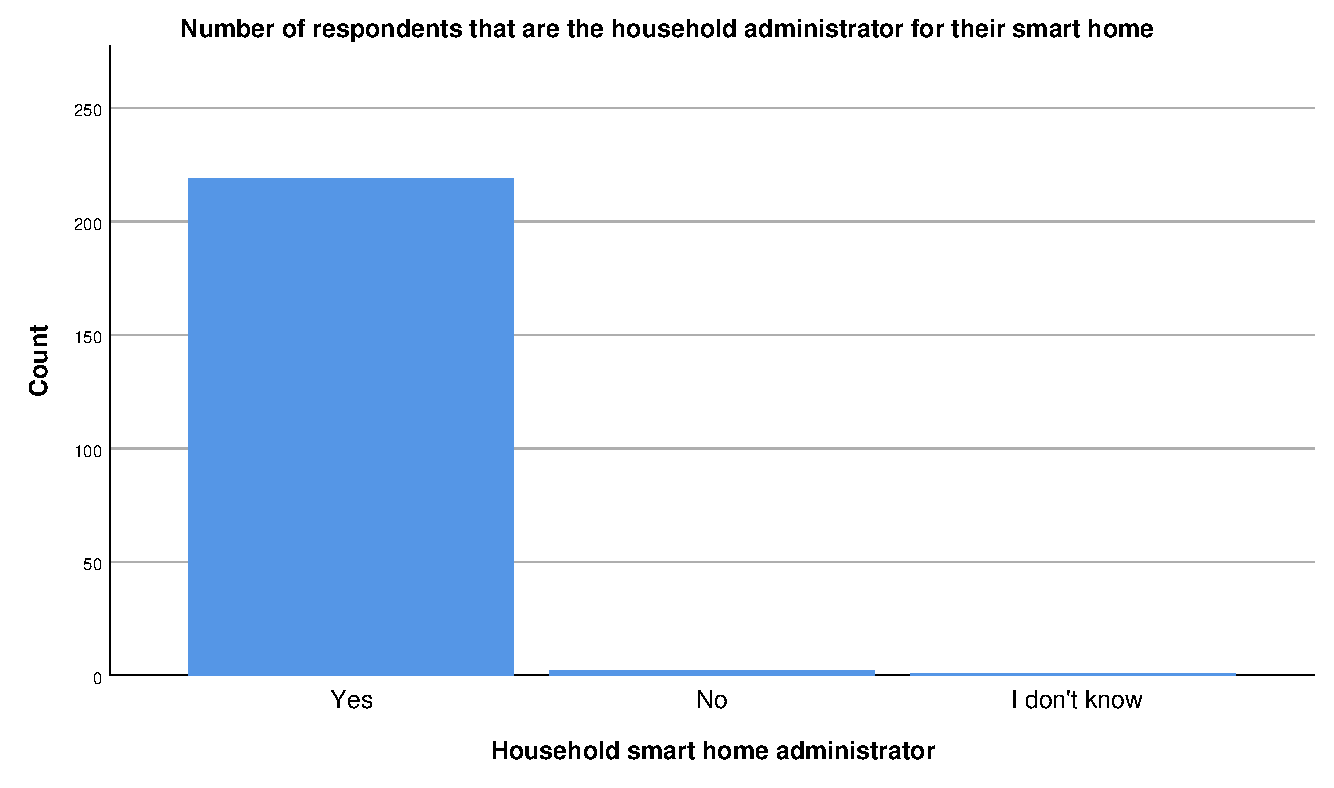
\includegraphics[scale=0.55]{figures/diagrams/administrator.pdf}
    \caption{Household administrators of their smart home}
    \label{fig:administrator}
\end{figure}

Out of the total of 222 people who answered, 219 (98.6\%) of the respondents said that they were the smart home administrator of their household. Only 2 people said no, and the last one said that they did not know. This shows us that the people in this study are active users, and not passive ones. 

\subsection{Professional / hobby based background}
I asked a question to figure out if the respondents had a background in technology, either a professional one or as a hobby. My hypothesis was that most people would have a background in technology, since that is how you get exposed to and interested in devices like those in a smart home. From figure \ref{fig:background} below, we can see that most people does have a background in technology. 
\begin{figure}[!h]
    \centering
    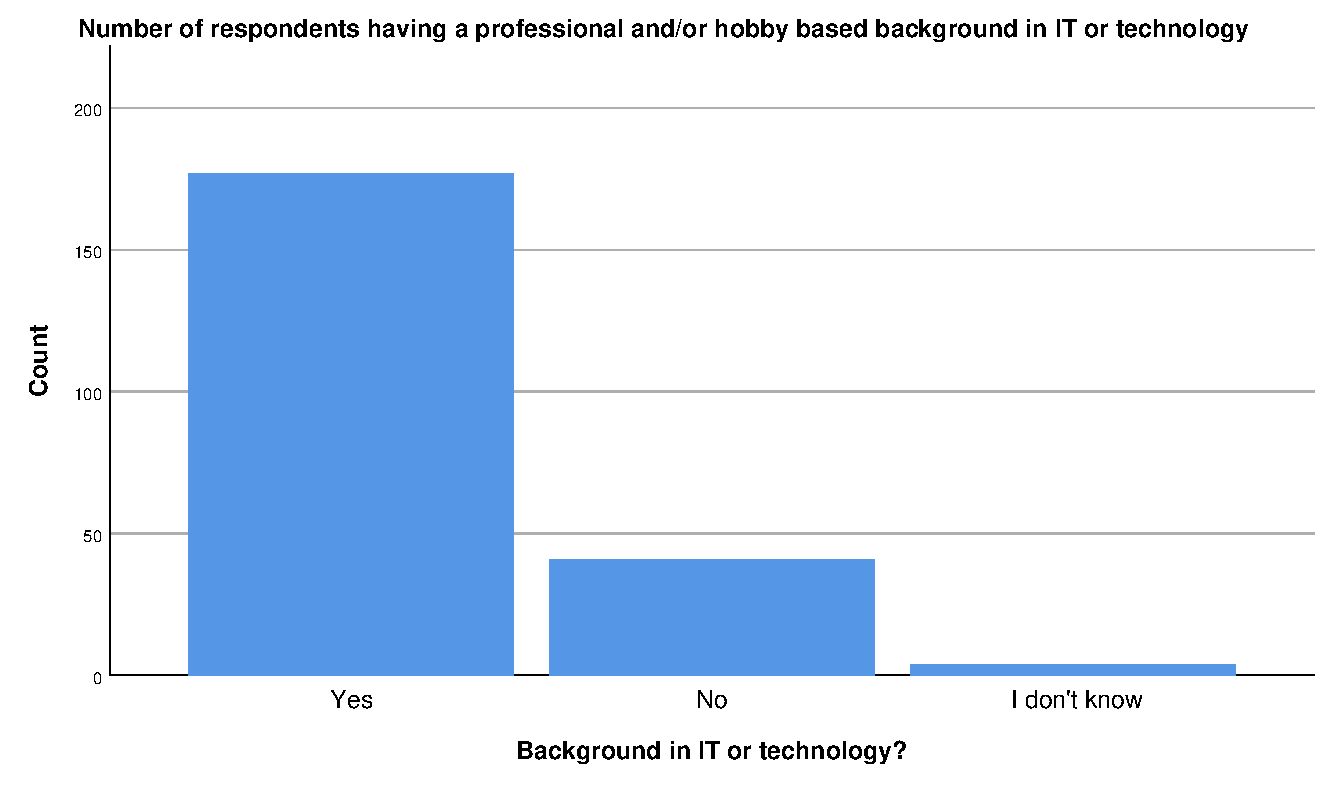
\includegraphics[scale=0.55]{figures/diagrams/background.pdf}
    \caption{The respondents background in IT or technology}
    \label{fig:background}
\end{figure}
Out of the total of 222 people who answered this question, 177 respondents (79.7\%) said yes and 41 people (18.5\%) answered no. The last four people said that they did not know. This shows us that the sample consist of many people from a technological background. 

\subsection{Knowledge of subjects}
In addition to the previous questions, I also wanted to assess the respondents knowledge on certain subjects relating to smart home security. This is of course only self-reported knowledge. My hypothesis was that they know a lot about technology and smart homes, but not that much about data security. We can see that the hypothesis was mostly correct based on figure \ref{fig:knowledge} below. 
\begin{figure}[!h]
    \centering
    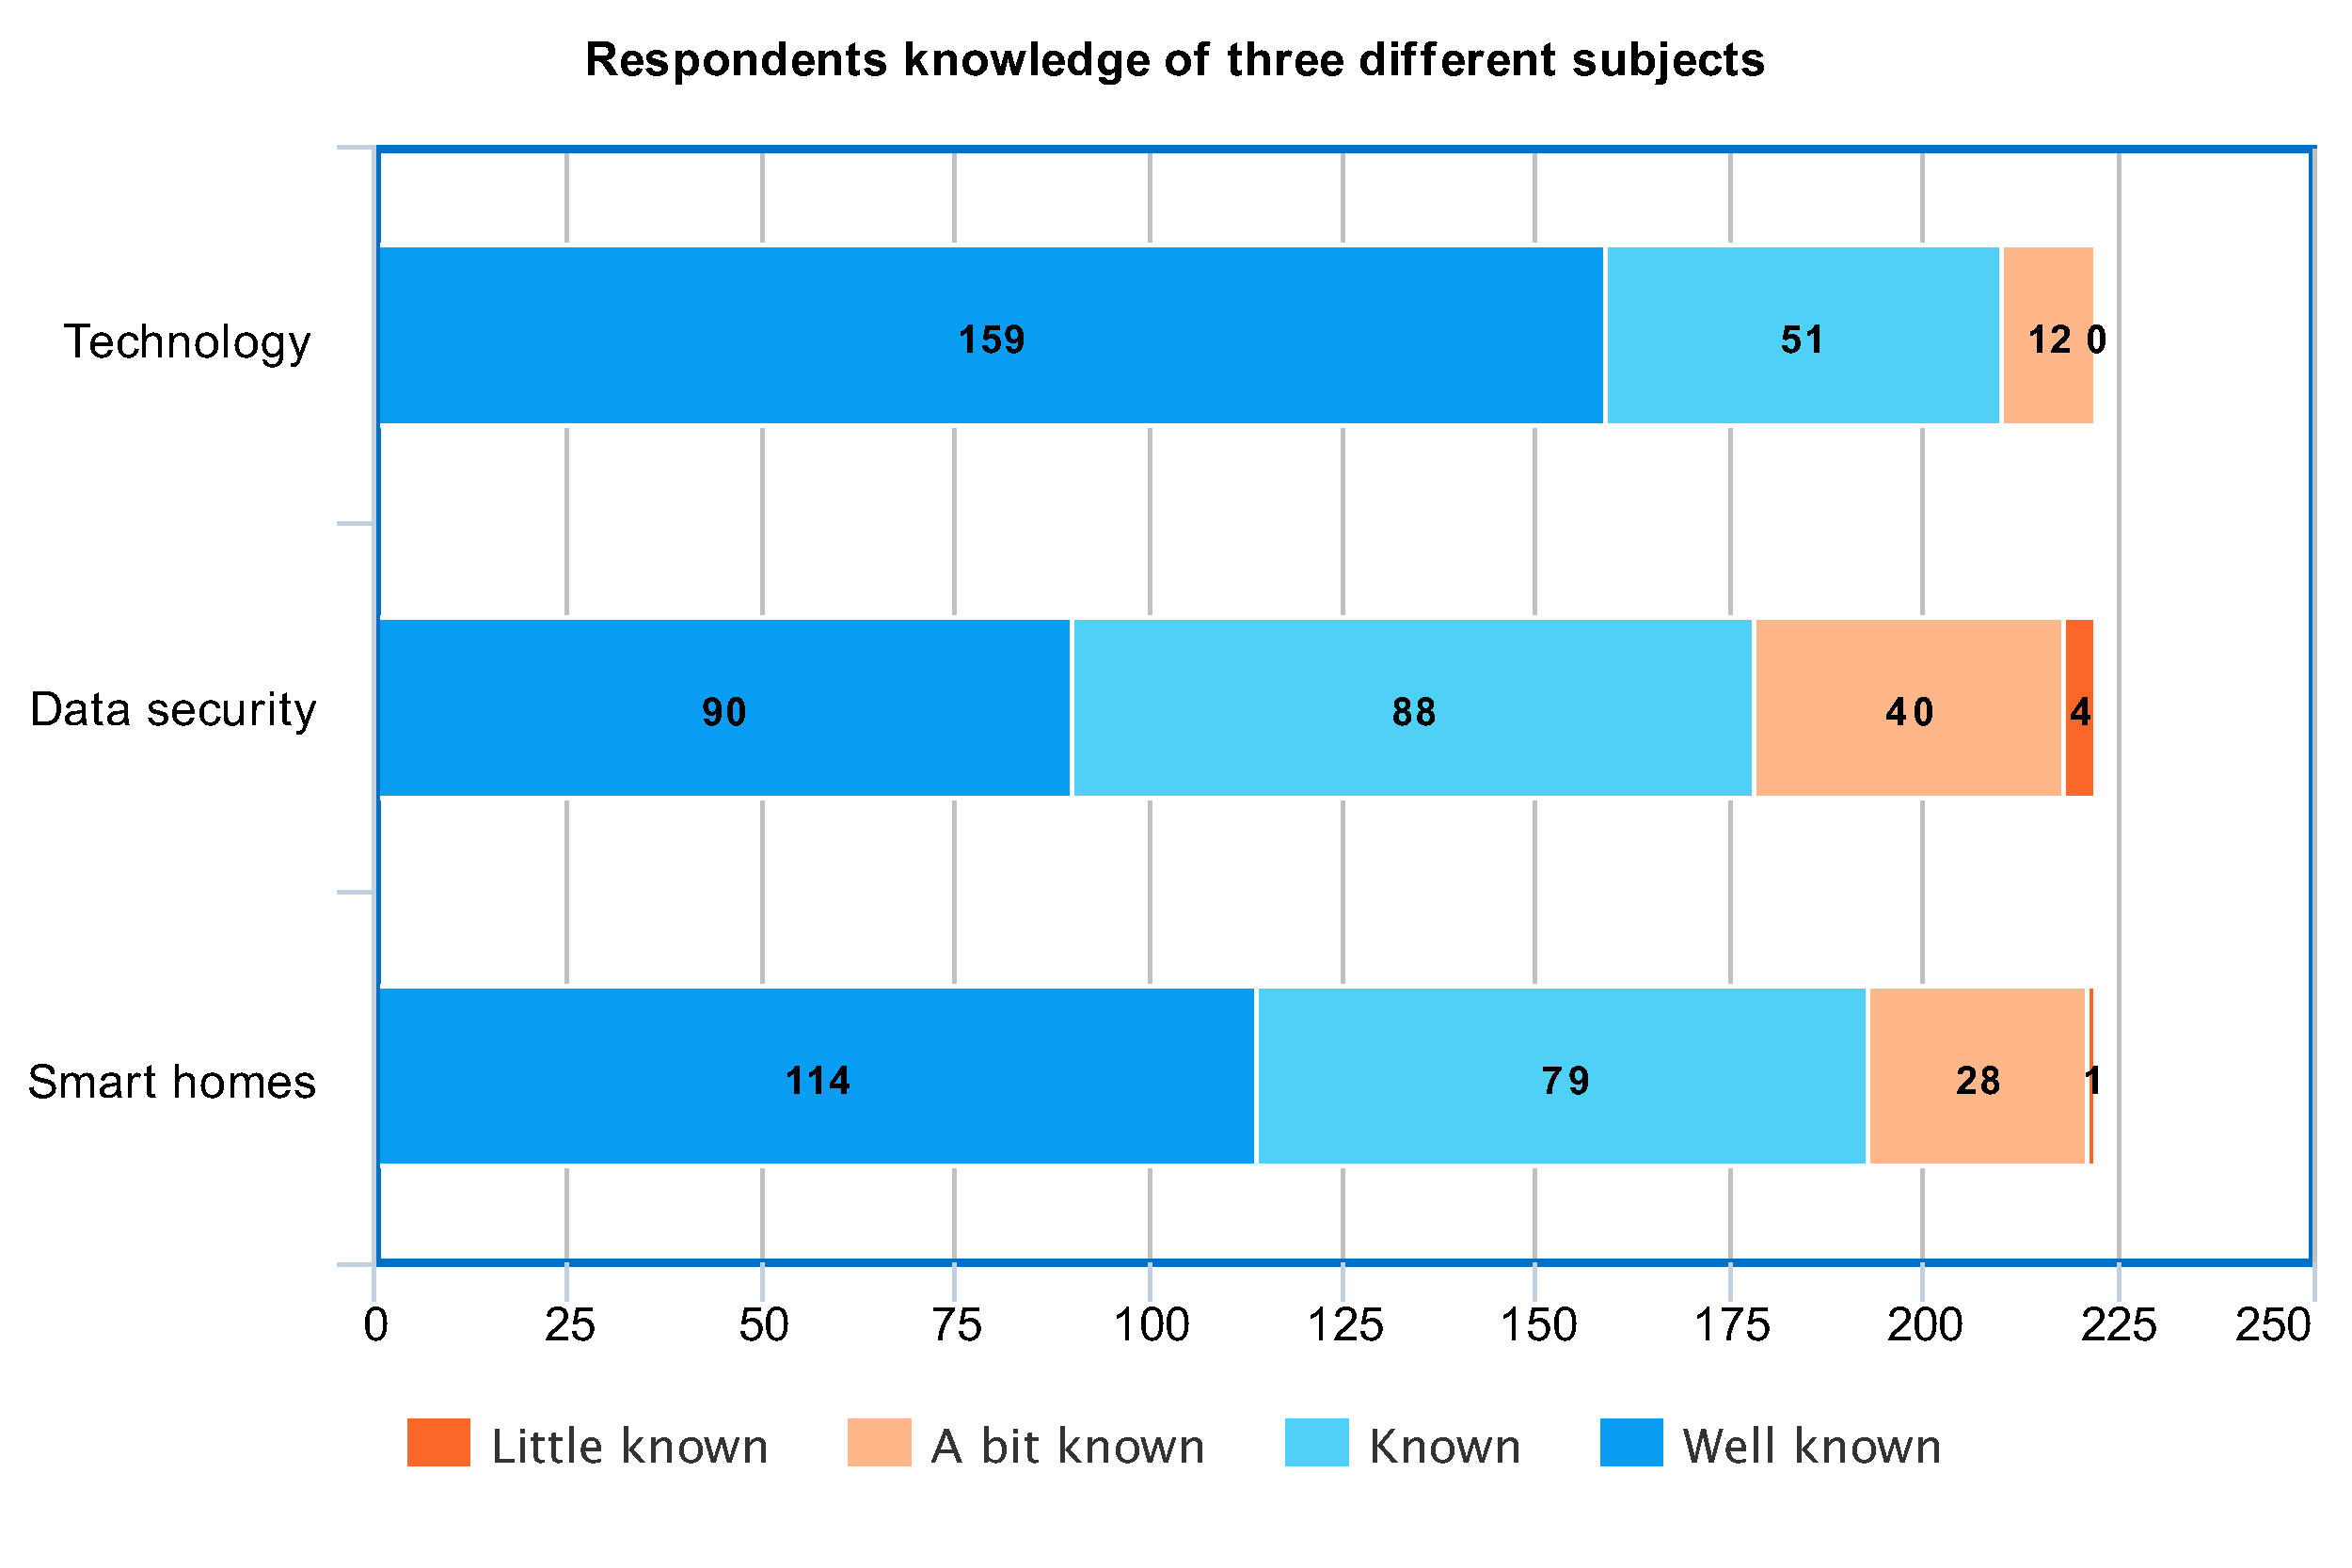
\includegraphics[scale=0.3]{figures/diagrams/knowledge.pdf}
    \caption{The respondents knowledge of three different subjects}
    \label{fig:knowledge}
\end{figure}

159 (71.6\%) of the respondents answered that they know technology well, while another 51 (23\%) claims to know it. This amounts to 94.6\% of the respondents alone. Regarding data security, 90 people (40.5\%) said they know it well, while 88 people (39.6\%) responded that it was known to them. This is considerable less than with technology, but still fairly good as it amounts to around 80.2\%. Lastly, 114 respondents (51.4\%) answered that smart homes was well known to them, while 79 people (35.6\%) responded that it was known. This is more than data security, however still significantly less than technology. While still being partly correct in my hypothesis, it was surprising that the knowledge of smart homes was not closer to technology for a sample specifically interested in smart homes. This could have many explanations, such that there are people that joined the Facebook group in order to learn, so they might not be experts yet. Another explanation could be that they underestimate their own expertise, and overestimate what they do not know. This has been proven to be the case in multiple studies previously \cite{Ehrlinger2008} \cite{MCCORMICK1986205}. 

\section{Security awareness of the respondents}
In this section I will perform univariate analysis on the questions in the main survey that includes data that can be used to describe the security awareness of the sample. This analysis is broken down into four parts: the respondents use of smart home devices, their credential management, knowledge of different smart home security aspects, and risk perceptions based on a few given risk scenarios. 

\subsection{Use of Smart Home Devices}
\label{subsec:use_smart_devices}
The first question aims to identify the respondents routines when it comes to regularly updating their smart devices. I had an hypothesis at the start that most people do update their devices, but that the majority wait a while before doing so. The results are visualised in figure \ref{fig:update} below.
\begin{figure}[!h]
    \centering
    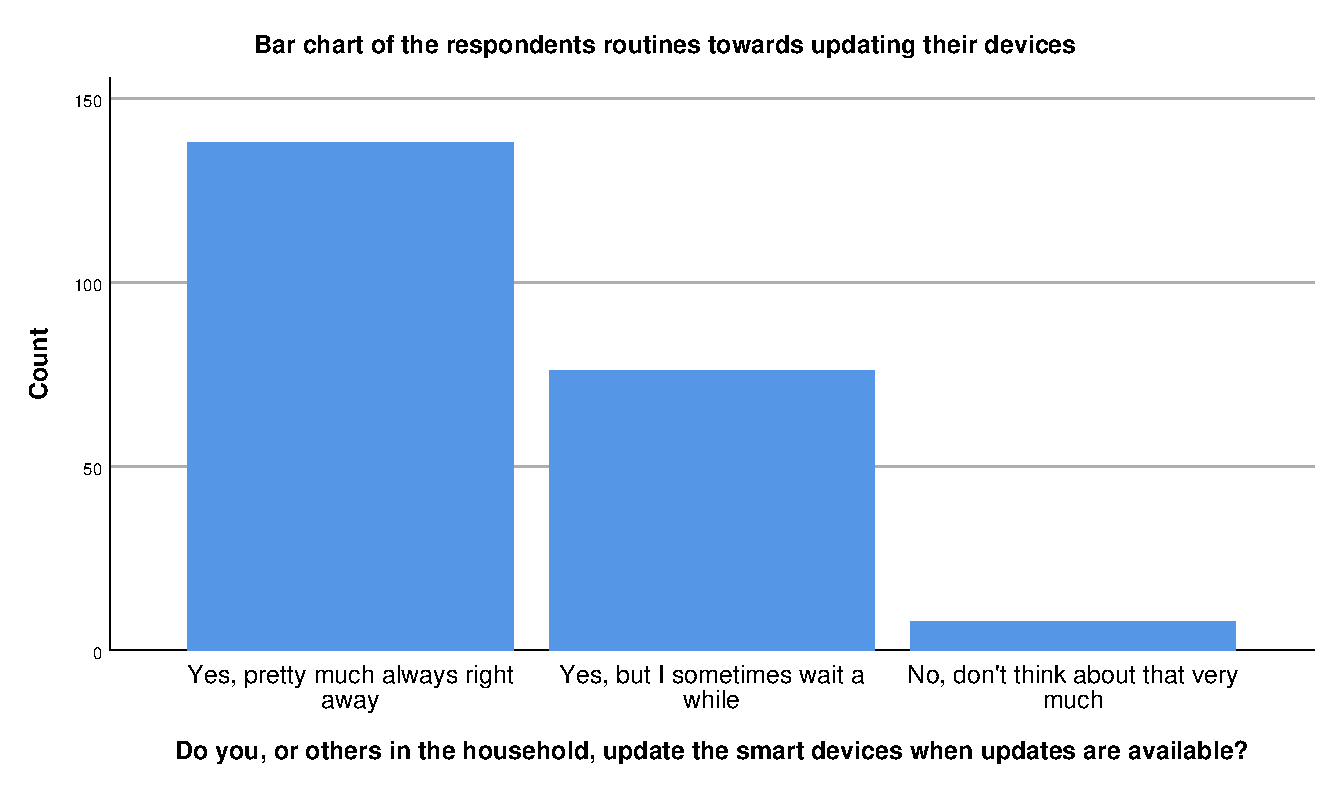
\includegraphics[scale=0.55]{figures/diagrams/update.pdf}
    \caption{The respondents routines towards updates their devices}
    \label{fig:update}
\end{figure}
A total of 138 people (62.2\%) answered that they pretty much always update their devices right away, and 76 people (34.2\%) said they do update their devices regularly, however they sometimes wait a while. Only 8 people (3.6\%) responded that they do not think about updating their devices that much. This did not confirm my hypothesis, and shows that the majority actually try to update their devices regularly, even though a significant portion (34.2\%) sometimes waits a while before doing so. 

The next question aimed to quantify how many people actually interact with the settings and turn off features and services they do not use regularly. My initial hypothesis for this question was that most people did not turn off features they do not use. The results from this question are displayed in figure \ref{fig:turn_off_features} below. 
\begin{figure}[!h]
    \centering
    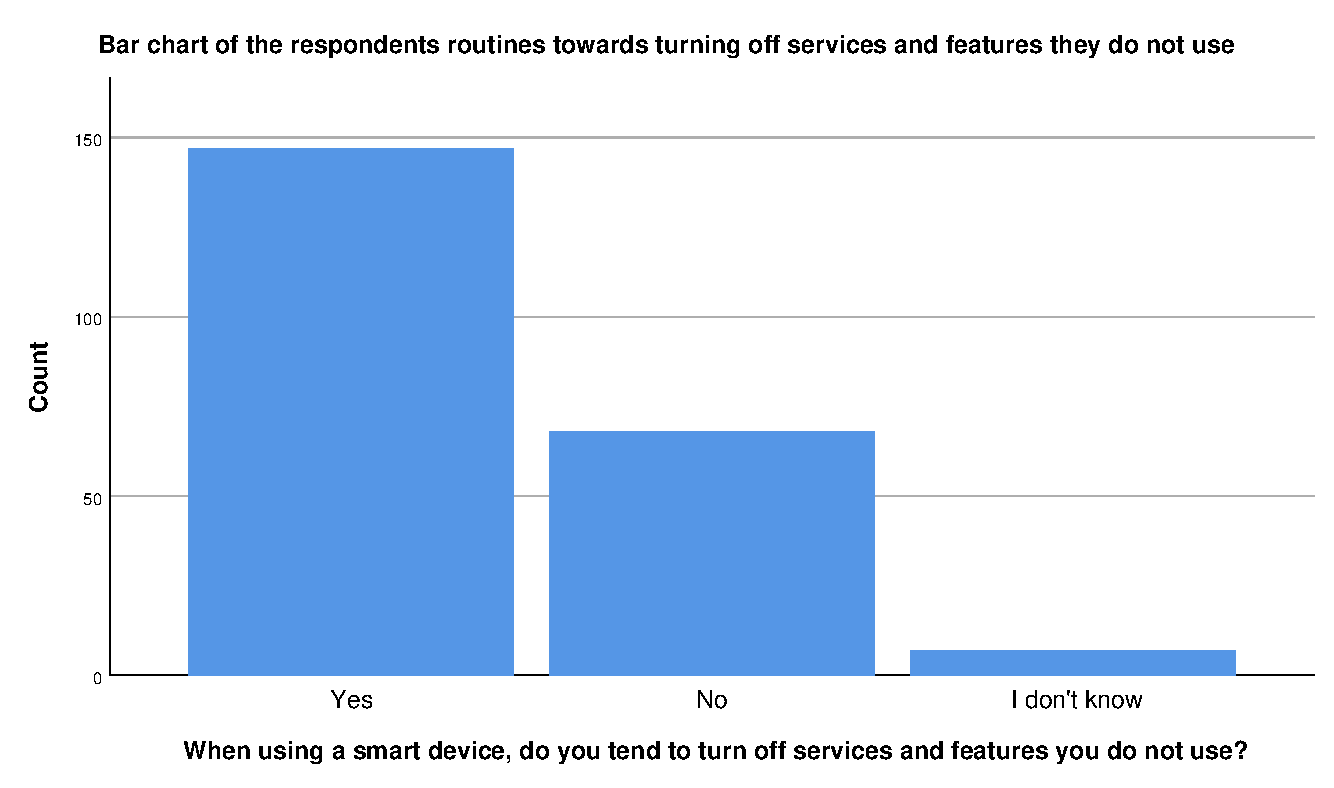
\includegraphics[scale=0.55]{figures/diagrams/turn_off_features.pdf}
    \caption{The respondents routines towards turning off features and services they do not use}
    \label{fig:turn_off_features}
\end{figure}
For this question, 147 people (66.2\%) confirmed that they turned off features and services they did not use, and 68 of the respondents (30.6\%) denied doing so. Only 7 people (2.3\%) did not know whether they did so or not. This is the opposite result to what I had as my hypothesis and shows that most people are mindful about what services they keep running that they do not need. However, this also shows that almost one third of my sample could have an amplified risk profile due to this. 

Some \cite{ENISA2015SmartHome} consider it best practise to segment their home network when you have multiple device types that that access your network, for example connecting smart devices to the network. I therefore asked the question if the respondents used a separate segment of their home network for their smart devices. My initial hypothesis was that most people did not segment their network for this purpose. The results are visualised in a bar chart in figure \ref{fig:separat_segment} below. 
\begin{figure}[!h]
    \centering
    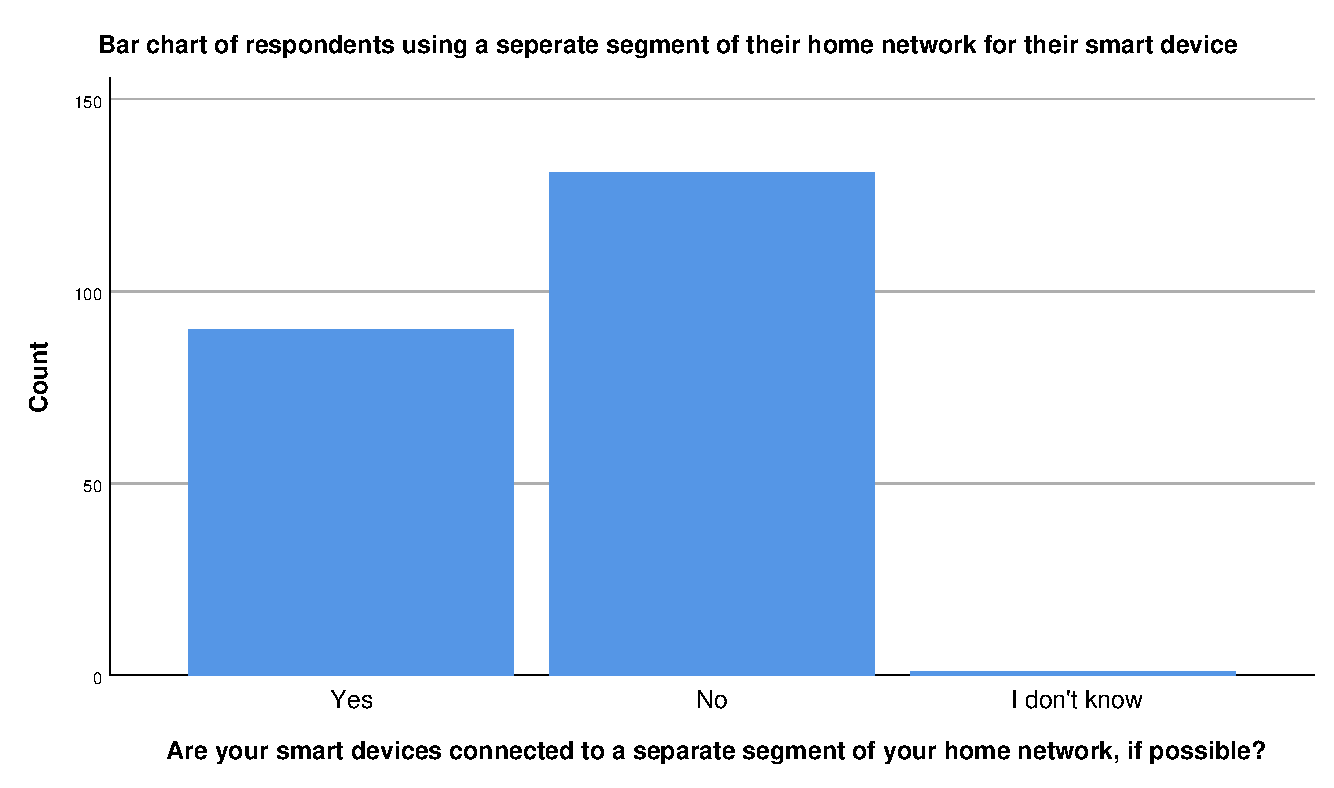
\includegraphics[scale=0.55]{figures/diagrams/separat_segment.pdf}
    \caption{The respondents routines towards connecting smart devices to a separate home network segment}
    \label{fig:separat_segment}
\end{figure}
The answers show us that 90 people (40.5\%) use a separate segment of their home network when connecting their devices to the network, and 131 people (59\%) does not. Only 1 person answered that they did not know. This confirms my hypothesis, however, it was a bit closer than what was initially expected. The results could indicate that most people either does not know that this is best practise, or that they lack the necessary networking knowledge to make it happen, despite it being much easier for a consumer to do than before. 

Another aspect I wanted to explore in regards to smart home device usage was the respondents routines towards changing their security and privacy settings. A significant part about security awareness is the conscious decisions you make about security and the risks you choose to accept or not. Privacy concerns have actually gotten some attention from the media lately \cite{nrk_smarthoytaler} \cite{nrk_avslort}, so my hypothesis is that the majority actually change or at least validate their privacy and security settings, either to give out more or less information. The results are visualised in figure \ref{fig:settings} below. 
\begin{figure}[!h]
    \centering
    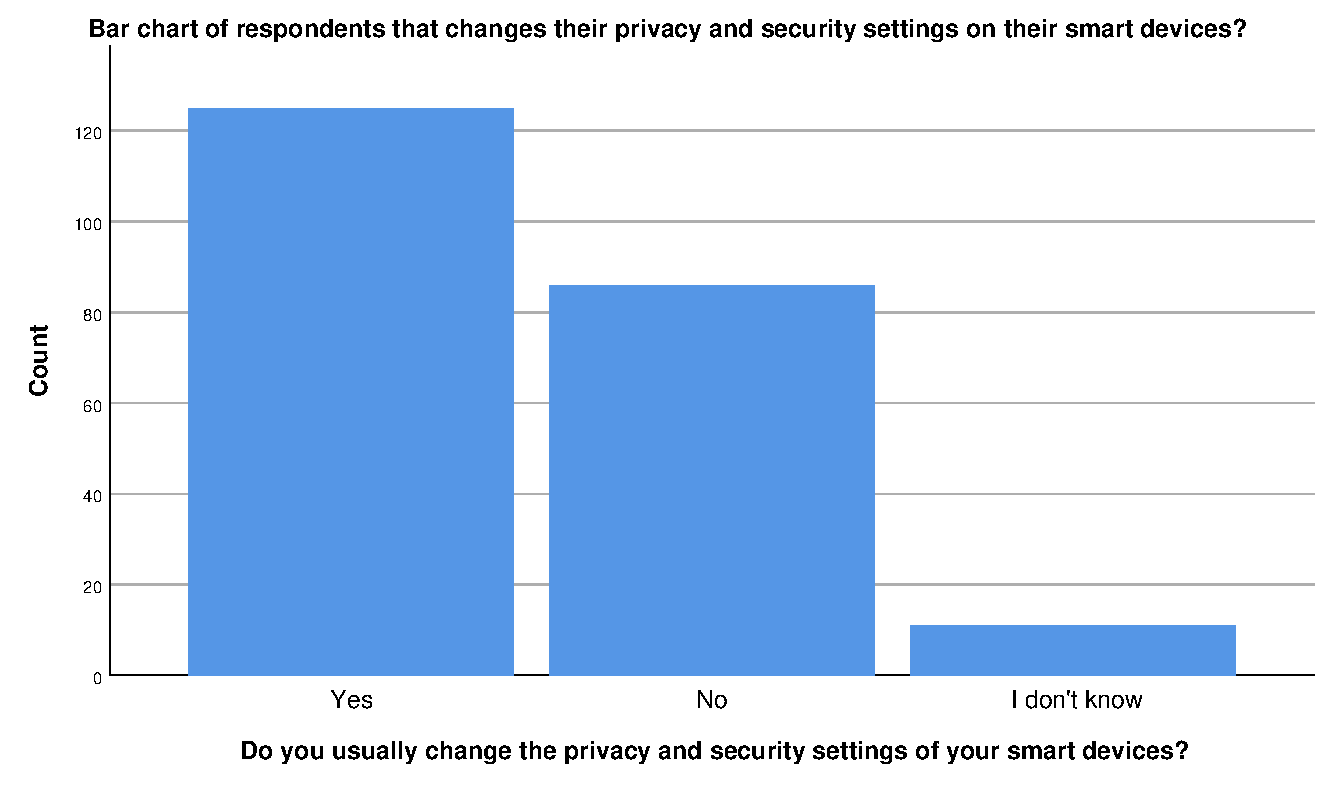
\includegraphics[scale=0.55]{figures/diagrams/settings.pdf}
    \caption{The respondents routines towards changing their security and privacy settings}
    \label{fig:settings}
\end{figure}
From the sample we observe that 125 people (56.3\%) answered that they do change the privacy and security settings on their smart devices, and 86 people (38.7\%) answered that they did not. Only 11 people (5\%) responded that they did not know. This confirms my hypothesis that the majority care about changing their privacy and security settings, although not by a large margin. Even though almost 40\% does not change their settings at all, we do not know whether this is an accepted risk, or just due to not knowing what data is being shared or not caring. This could be interesting to look at further as a bivariate analysis.

Lastly for device usage, I wanted to explore the respondents preference in what they use to connect their smart devices to the internet, and asked them if they preferred cable or wireless where possible. My hypothesis was that they would largely prefer wireless, since it would be easier to set up, and less hassle without cables lying around. Of course there are devices that only connect using one of the methods, and that is why I included ``where possible'' in the answers. The results are shown in figure \ref{fig:connect_internet} below. 
\begin{figure}[!h]
    \centering
    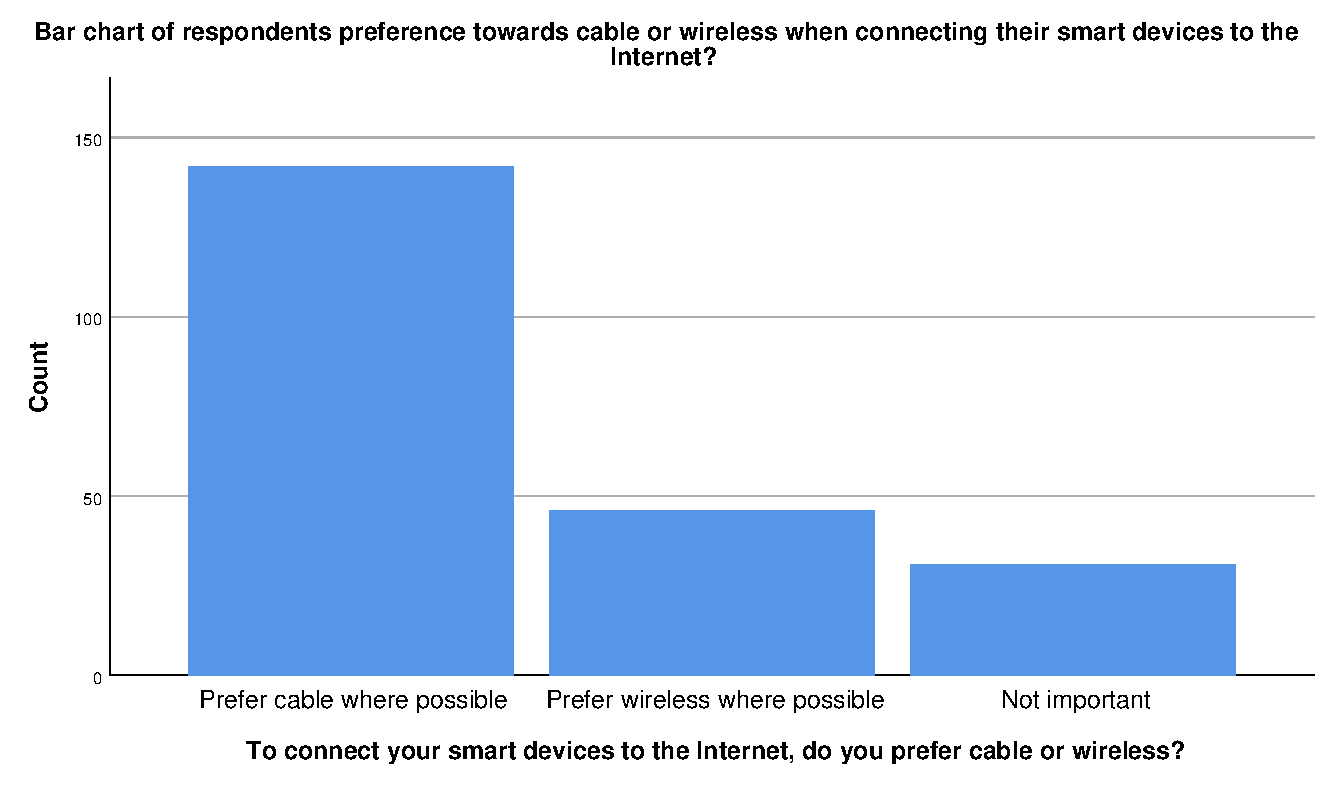
\includegraphics[scale=0.55]{figures/diagrams/connect_internet.pdf}
    \caption{The respondents preference for cable or wireless when connecting their smart devices to the Internet}
    \label{fig:connect_internet}
\end{figure}
Surprisingly, 142 people (64\%) preferred cable, and 46 people (20.7\%) preferred wireless. Also, 31 respondents (14\%) answered that it was not important to them how they connected their devices to the internet. The last 3 people answered that they had some other thoughts on the matter, with one of them specified in freetext that their devices was not connected to WAN, and another that none of his smart home devices are allowed access to internet. The last person did not include any additional thoughts. According to ENISA \cite{ENISA2015SmartHome}, the best practise is to use cable where possible, so this is not a pitfall many people fall into. 

\subsection{Credential management}
One thing I wanted to explore about peoples password routines was whether they changed the default password on the smart devices after purchase. Many products prompts the user to set or change the password after initialisation. Therefore, my hypothesis is that a large majority do change the default password on recently purchased devices. The results are displayed in figure \ref{fig:standard_password} below. 
\begin{figure}[!h]
    \centering
    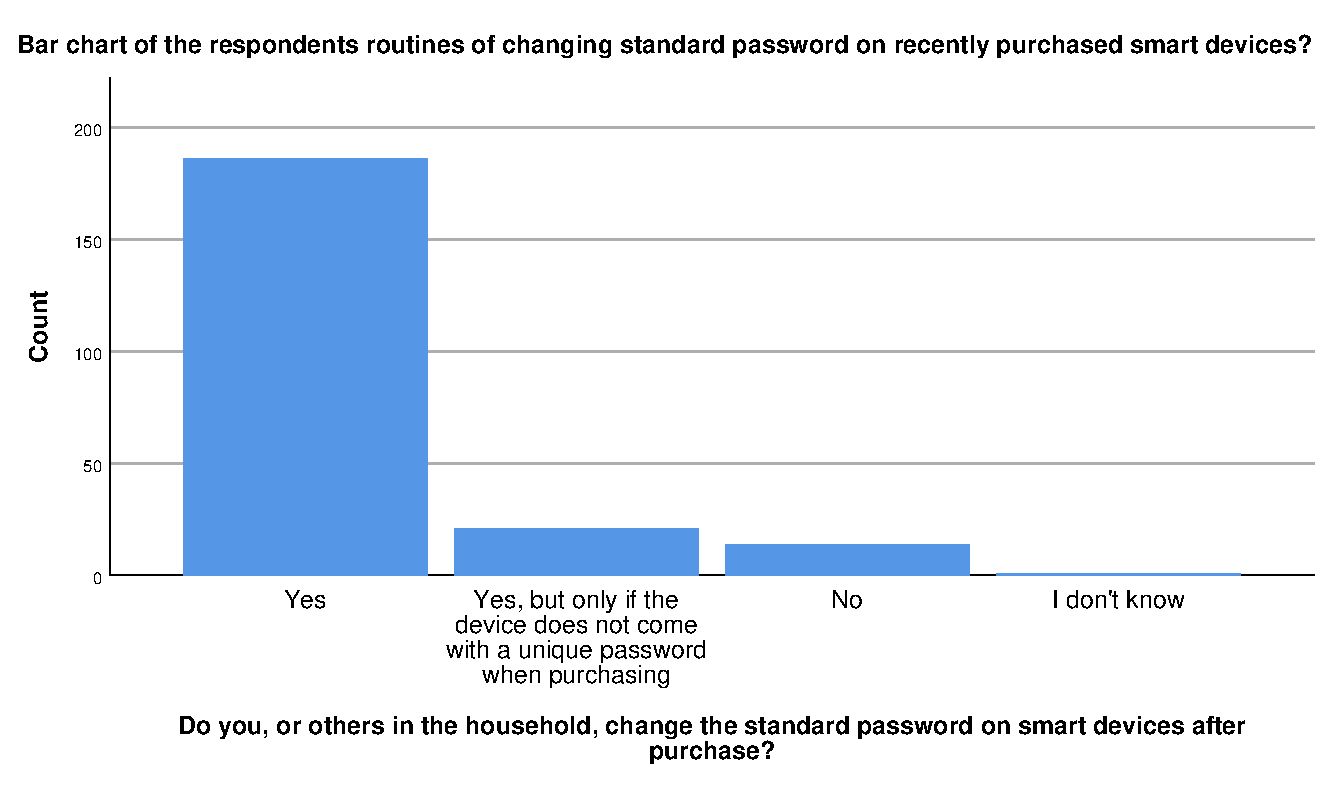
\includegraphics[scale=0.55]{figures/diagrams/standard_password.pdf}
    \caption{The respondents routines towards changing standard passwords}
    \label{fig:standard_password}
\end{figure}
A total of 186 people (83.8\%) answered that they did change the default password, while 21 (9.5\%) said they did so only if the device did not come with a unique password when purchased. Only 14 people (6.3\%) answered that they did not change the password, and the last person was not sure. This shows that my hypothesis was correct in that a large majority do change the default password, and it was in fact over 90\% of the respondents in total. 

Next I wanted to know if my sample used a password manager to store their password in. Once again, this was asked as a binary type yes/no question, however, I allow an option for people who does not know about password managers. My hypothesis was that most people do not use password managers, and also that a significant number does not know of the service in the first place. The results from the question are visualised in figure \ref{fig:password_manager} below. 
\begin{figure}[!h]
    \centering
    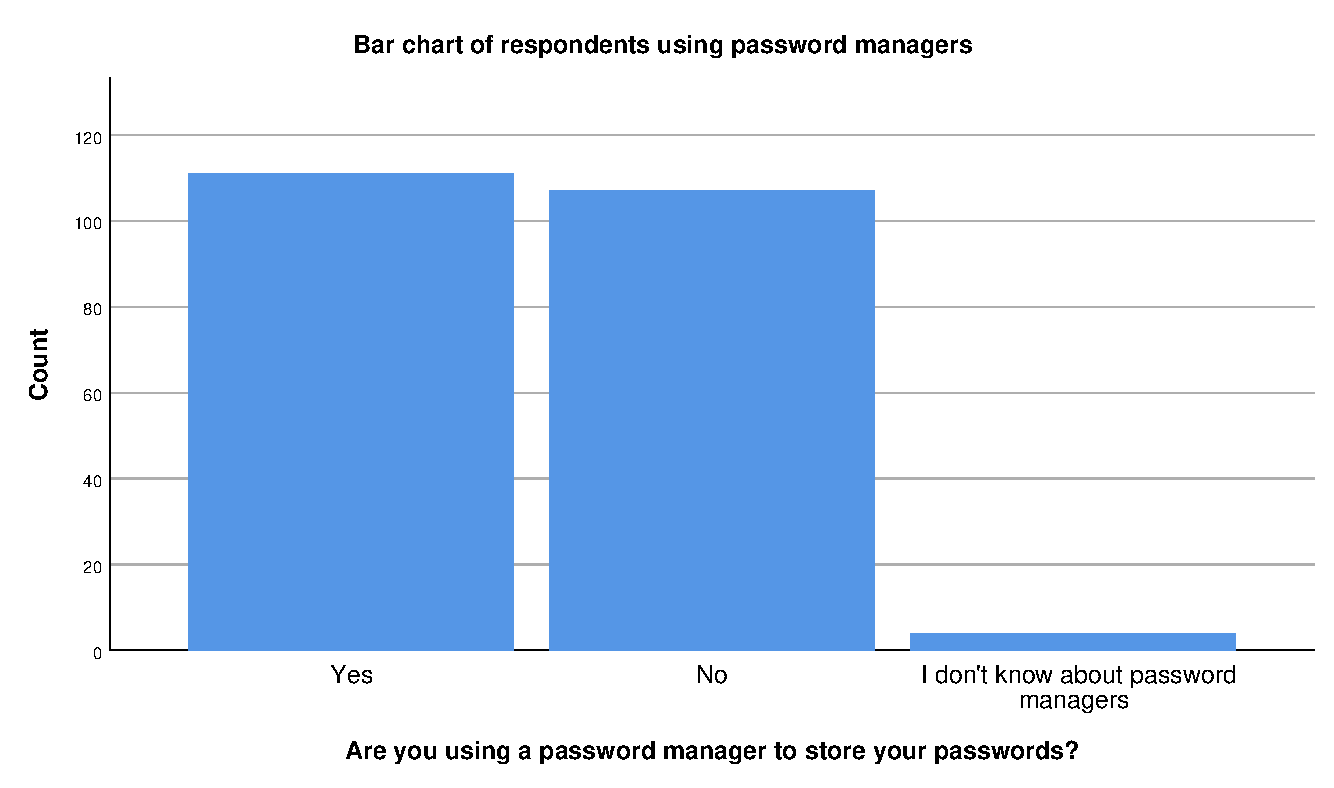
\includegraphics[scale=0.55]{figures/diagrams/password_manager.pdf}
    \caption{The respondents routines towards using password managers}
    \label{fig:password_manager}
\end{figure}
111 of the respondents (50\%) answered that they do use a password manager to store their passwords in, and 107 people (48.2\%) do not. Only 4 people (1.8\%) admitted to not knowing of password managers. It was surprising that exactly half used a password manager, so my hypothesis was proven wrong. It was also interesting to see that so few people did not know about the service. This could be because they did not want to admit not knowing about it, and just answered no instead. And technically that is still the truth, so this might be a limitation for this question. 

In the last question regarding credential management I wanted to assess the respondents routines when it comes to password reuse. Password reuse could lead to higher consequence if the credentials were to get compromised due to an event. Suddenly, an intruder would not only gain access to one service or device, but possibly multiple. My hypothesis was that the majority understands the risks of password reuse, and therefore do not use the same passwords. The results are shown in figure \ref{fig:password_reuse} below. 
\begin{figure}[!h]
    \centering
    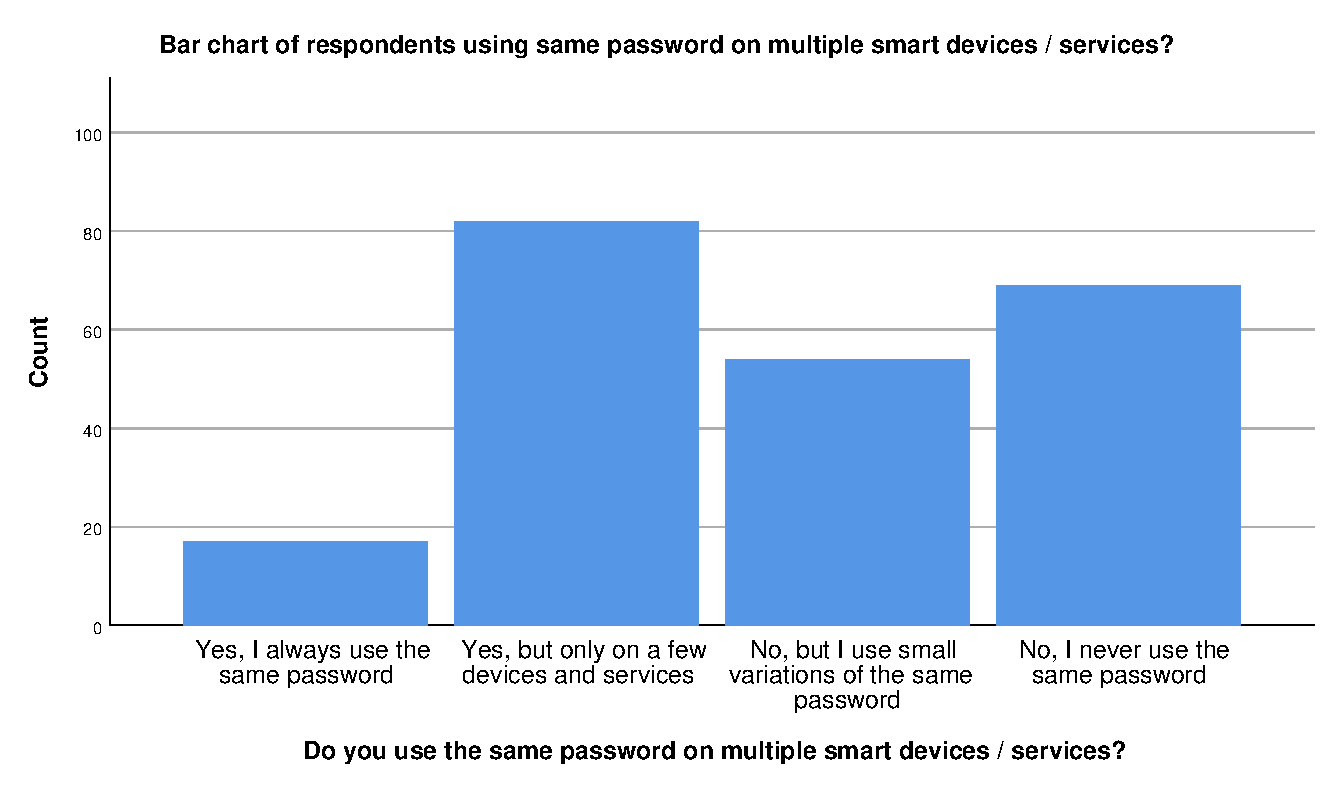
\includegraphics[scale=0.55]{figures/diagrams/password_reuse.pdf}
    \caption{The respondents routines towards using password on multiple devices/services}
    \label{fig:password_reuse}
\end{figure}
The descriptive statistics show us that only 17 people (7.7\%) admitted to always using the same password, while 82 people (36.9\%) reused their password only on a couple of services and devices. Furthermore, 54 people (24.3\%) responded that they did not reuse the same password, however they used small variations of the same base password. Lastly, the remaining 69 people (31.1\%) never used the same password. This shows us that a worrying number of people reuse their password, although the majority of them only reused it on a few services, which would reduce the potential impact of a credential leak. My hypothesis was mostly true, however a sizeable portion used variations of the same password, which is not ideal, but could be adequate depending on the strength of the base password. This could also make it easier to remember if you do not use a password manager, while at the same time retaining password strength. 

\subsection{Knowledge of smart home security aspects}
I asked the respondents to rate their knowledge of three different aspects relating to the security awareness of smart homes, ranging from little known to well known. The results are displayed in figure \ref{fig:knowledge_security} below. 
\begin{figure}[!h]
    \centering
    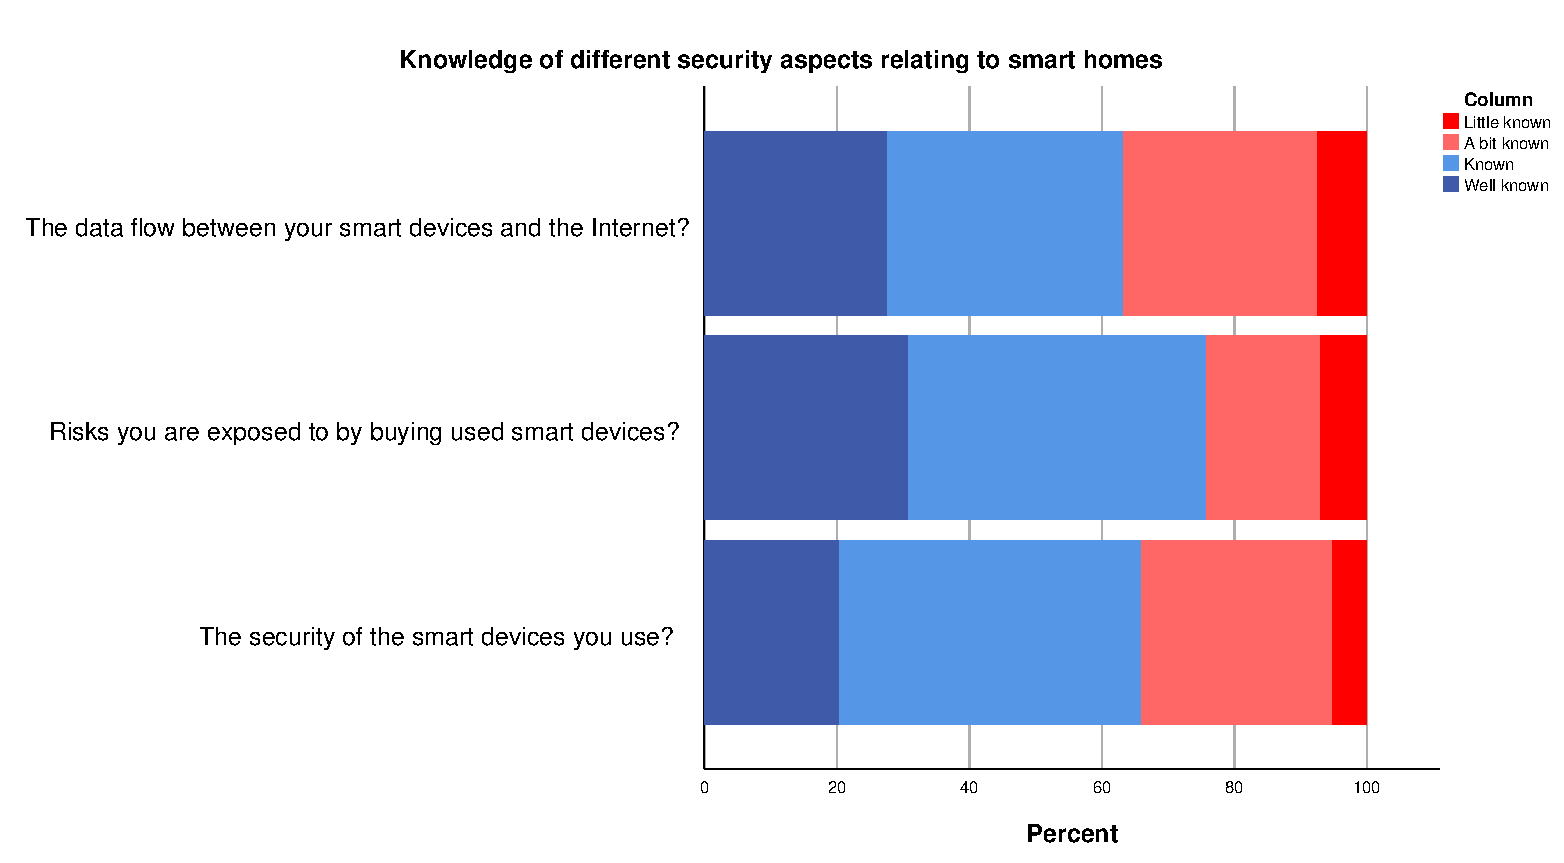
\includegraphics[scale=0.45]{figures/diagrams/knowledge_security.pdf}
    \caption{Knowledge of different security aspects relating to smart homes}
    \label{fig:knowledge_security}
\end{figure}
Regarding their self-proclaimed knowledge of the data flow between the smart devices and the internet, 140 people (63.1\%) claimed that it is known or well known to them, while 82 people (36.9\%) claimed to know little or just a bit.
When it comes to risks they are exposing themselves to when buying used smart devices, 168 people (75.6\%) claims that it is either known of well known, while only 44 people (24.4\%) claims to know little or just a bit. 
The last question was how well the respondents know the security of the smart devices they use, in which 146 people (65.8\%) claims to either know it or know it well, while 76 people (34.2\%) claims to know little or just a bit. 
We can see from the stacked bar chart, and the descriptive statistics the majority claims to at least know of these security awareness aspects, in which risks when buying used devices stands out as slightly more known among the respondents. 

\subsection{Risk perceptions of the respondents}
\label{subsec:risk_perception}
In the last set of questions I asked the respondents assess their perceived risk according to a set of risk scenarios. The respondents could choose a risk score from 1 to 6, where 1 equals to low risk and 6 equals to high risk. In table \ref{tab:risk_perception_desc} below, the mean scores are listed for all scenarios, together with the standard deviation of the respondents. 

\begin{table}[!h]
\centering
\begin{tabular}{|l|r|r|r|r|r|}
\hline
\multicolumn{6}{|c|}{{\color[HTML]{010205} \textbf{Descriptive Statistics of Perceived Risk}}} \\ \hline
{\color[HTML]{264A60} } &
  \multicolumn{1}{c|}{{\color[HTML]{264A60} N}} &
  \multicolumn{1}{c|}{{\color[HTML]{264A60} Min}} &
  \multicolumn{1}{c|}{{\color[HTML]{264A60} Max}} &
  \multicolumn{1}{c|}{{\color[HTML]{264A60} Mean}} &
  \multicolumn{1}{c|}{{\color[HTML]{264A60} Std. Dev.}} \\ \hline
\cellcolor[HTML]{E0E0E0}{\color[HTML]{264A60} \begin{tabular}[c]{@{}l@{}}1. One or more of your \\ smart devices gets infected \\ by malicious software\end{tabular}} &
  {\color[HTML]{010205} 222} &
  {\color[HTML]{010205} 1} &
  {\color[HTML]{010205} 6} &
  {\color[HTML]{010205} 2.77} &
  {\color[HTML]{010205} 1.235} \\ \hline
\cellcolor[HTML]{E0E0E0}{\color[HTML]{264A60} \begin{tabular}[c]{@{}l@{}}2. An unauthorized person \\ gets access to login details \\ for one or more smart devices\end{tabular}} &
  {\color[HTML]{010205} 221} &
  {\color[HTML]{010205} 1} &
  {\color[HTML]{010205} 6} &
  {\color[HTML]{010205} 2.90} &
  {\color[HTML]{010205} 1.502} \\ \hline
\cellcolor[HTML]{E0E0E0}{\color[HTML]{264A60} \begin{tabular}[c]{@{}l@{}}3. An unauthorized person \\ breaks into the house and \\ steals your   smart devices\end{tabular}} &
  {\color[HTML]{010205} 222} &
  {\color[HTML]{010205} 1} &
  {\color[HTML]{010205} 6} &
  {\color[HTML]{010205} 1.97} &
  {\color[HTML]{010205} 1.192} \\ \hline
\cellcolor[HTML]{E0E0E0}{\color[HTML]{264A60} \begin{tabular}[c]{@{}l@{}}4. An unauthorized person \\ takes control of your \\ smart devices and uses them \\ to attack others\end{tabular}} &
  {\color[HTML]{010205} 222} &
  {\color[HTML]{010205} 1} &
  {\color[HTML]{010205} 6} &
  {\color[HTML]{010205} 2.49} &
  {\color[HTML]{010205} 1.361} \\ \hline
\cellcolor[HTML]{E0E0E0}{\color[HTML]{264A60} \begin{tabular}[c]{@{}l@{}}5. An unauthorized person \\ intercepts the network traffic \\ to your   smart devices\end{tabular}} &
  {\color[HTML]{010205} 222} &
  {\color[HTML]{010205} 1} &
  {\color[HTML]{010205} 6} &
  {\color[HTML]{010205} 2.71} &
  {\color[HTML]{010205} 1.382} \\ \hline
\cellcolor[HTML]{E0E0E0}{\color[HTML]{264A60} \begin{tabular}[c]{@{}l@{}}6. One or more smart devices \\ are accidentally rendered \\ unusable\end{tabular}} &
  {\color[HTML]{010205} 222} &
  {\color[HTML]{010205} 1} &
  {\color[HTML]{010205} 6} &
  {\color[HTML]{010205} 2.68} &
  {\color[HTML]{010205} 1.366} \\ \hline
\cellcolor[HTML]{E0E0E0}{\color[HTML]{264A60} \begin{tabular}[c]{@{}l@{}}7. An unauthorized person \\ gets remote access to one \\ or more of your smart devices\end{tabular}} &
  {\color[HTML]{010205} 222} &
  {\color[HTML]{010205} 1} &
  {\color[HTML]{010205} 6} &
  {\color[HTML]{010205} 2.75} &
  {\color[HTML]{010205} 1.391} \\ \hline
\cellcolor[HTML]{E0E0E0}{\color[HTML]{264A60} \begin{tabular}[c]{@{}l@{}}8. An unauthorized person \\ accesses personal information \\ through your smart devices\end{tabular}} &
  {\color[HTML]{010205} 222} &
  {\color[HTML]{010205} 1} &
  {\color[HTML]{010205} 6} &
  {\color[HTML]{010205} 2.82} &
  {\color[HTML]{010205} 1.531} \\ \hline
\end{tabular}
\caption{Descriptive statistics of perceived risk from 8 risk scenarios}
\label{tab:risk_perception_desc}
\end{table}
We can see from table \ref{tab:risk_perception_desc} that most risk scenarios have a mean score of between approximately 2.5 and 2.9, and a standard deviation of 1.2 to 1.5. The risk scenario that stands out the most is breaking into the house, as it only has a mean score of 1.97, the lowest of the bunch, together with the lowest standard deviation at 1.192. At the upper end we have loss of login details at a mean of 2.9, with a standard deviation of 1.502. 

The results are displayed graphically in figure \ref{fig:risk perception} below, and is displayed based on the percentage of answers each risk score got. 
\begin{figure}[!h]
    \centering
    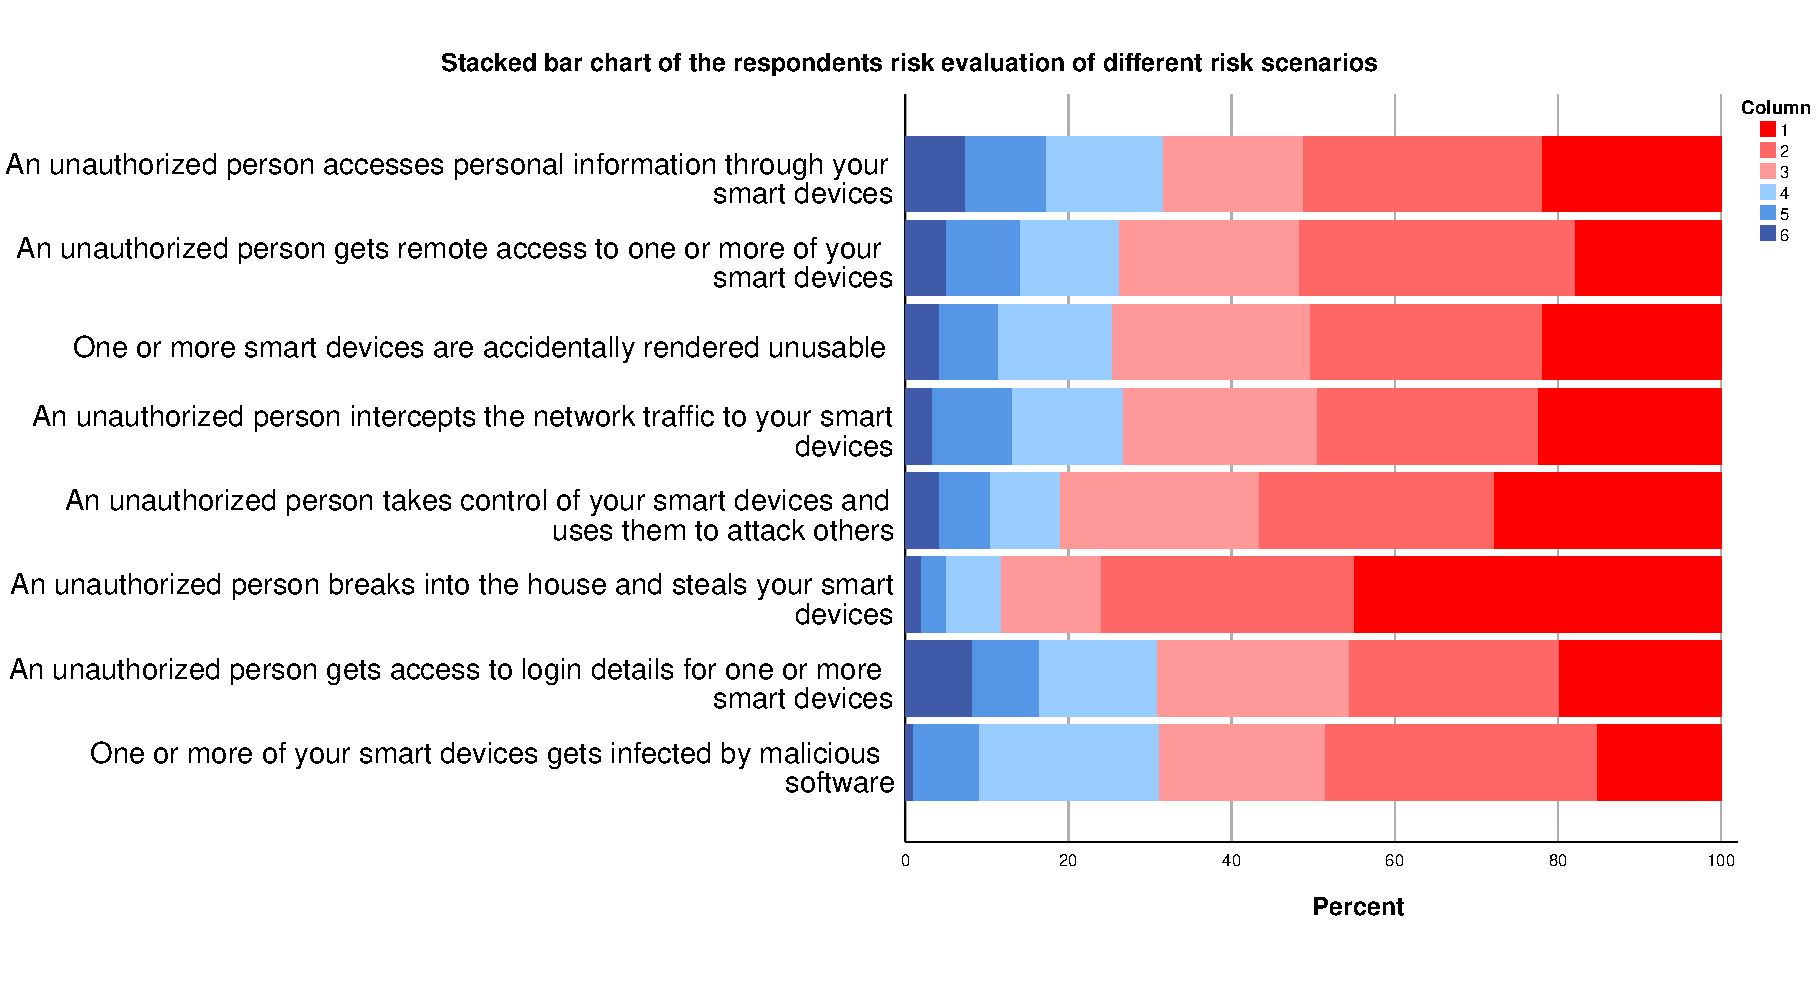
\includegraphics[scale=0.4]{figures/diagrams/risk_perception.pdf}
    \caption{Respondents risk evaluation of different risk scenarios}
    \label{fig:risk perception}
\end{figure}

\section{Bivariate analysis}
In this section I will perform bivariate analysis on my main sample. I started by analysing demographics as the independent variable, which includes age, education level, and county. Based on the previous analysis in section \ref{subsec:gender}, I was not able to do bivariate analysis on gender, and in my analysis there were no significant findings regarding county as an independent variable. 

\subsection{Age differences}
In my analysis of the differences in age groups I found that there were significant differences between the groups in mainly three different questions. The result of the ANOVA in figure \ref{fig:anova_age} below, shows us that the answers between the groups are significantly different since I am using the threshold of P = 0.05. 
\begin{figure}[!h]
    \centering
    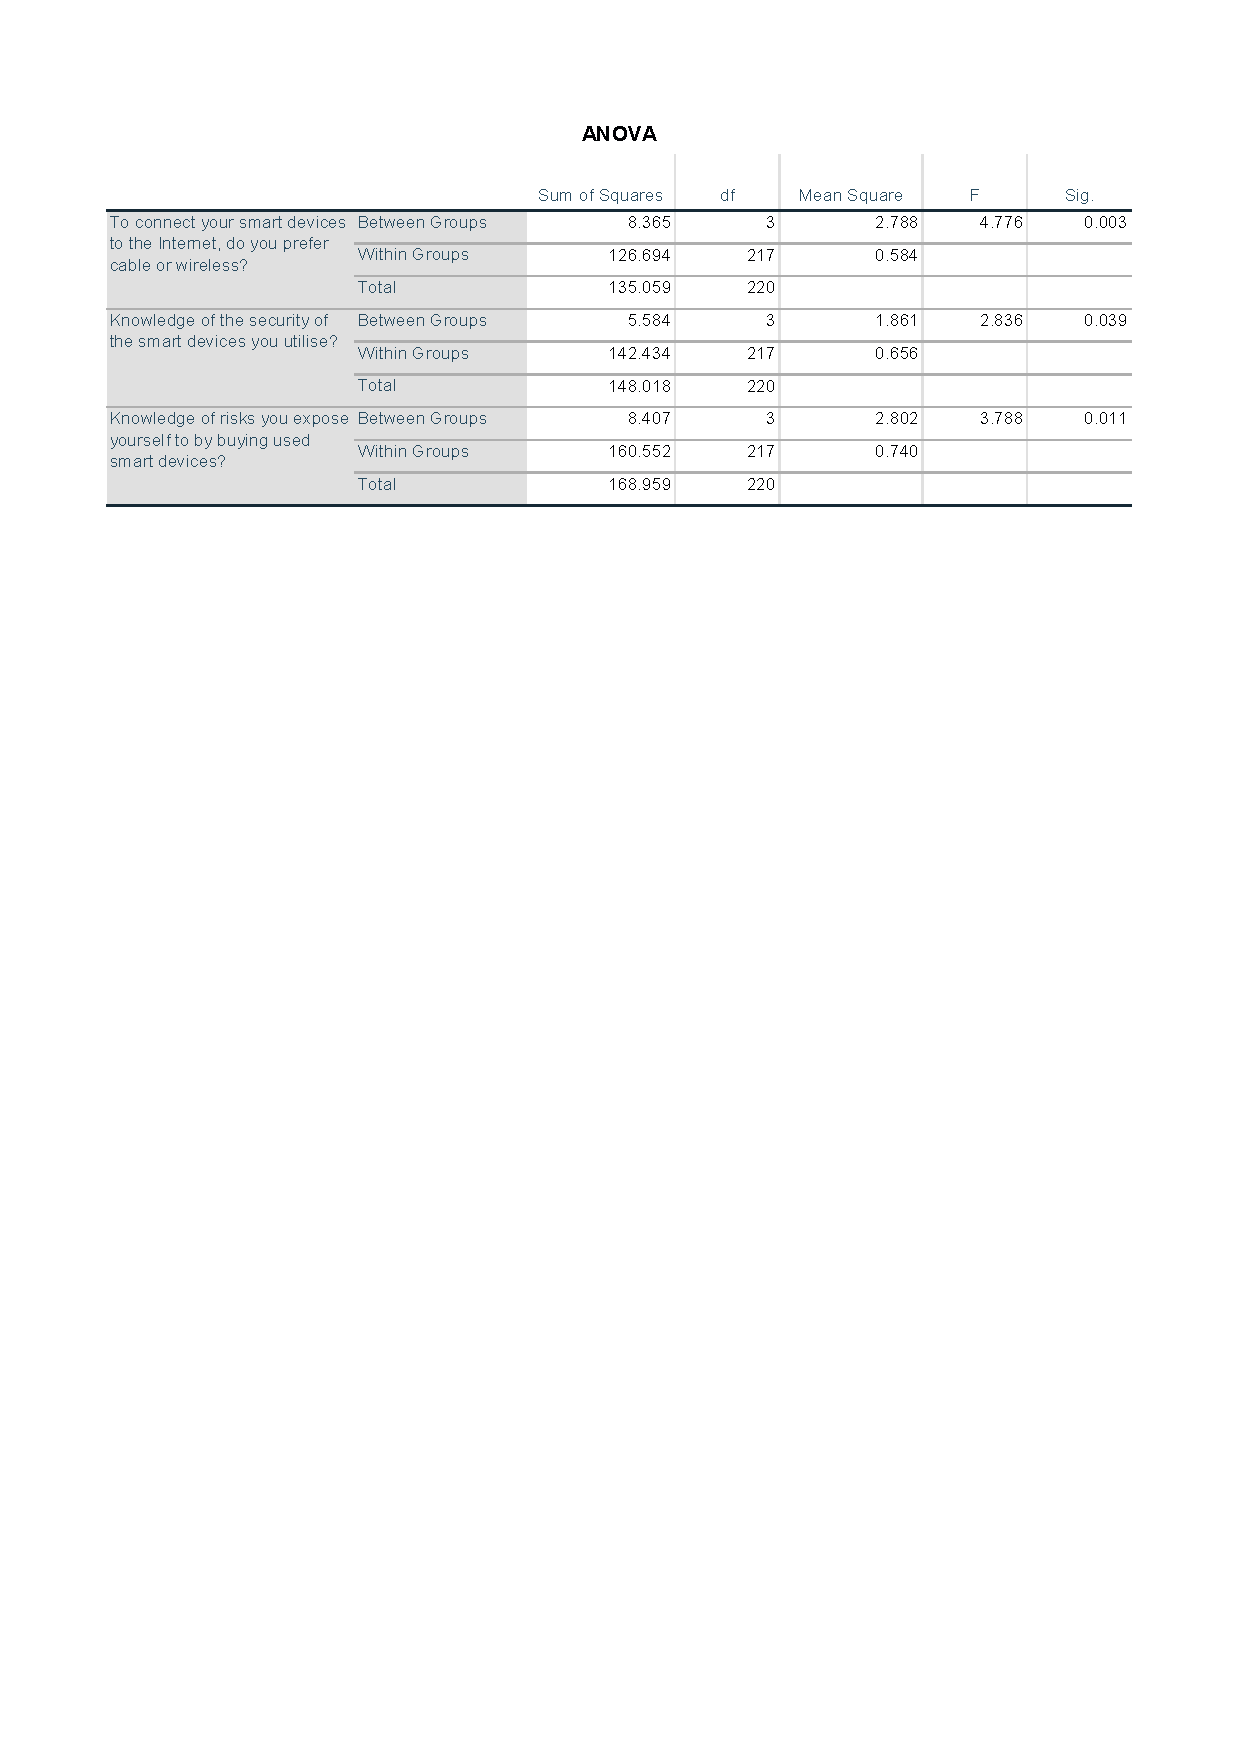
\includegraphics[scale=0.7]{figures/tables/anova_age.pdf}
    \caption{ANOVA of age up against other variables}
    \label{fig:anova_age}
\end{figure}
If we look further at the descriptive statistics I have included in the appendix \ref{fig:anova_age_desc}, we can see that the age group that are older than 50 is more likely to score higher in their knowledge of the risks of buying used smart devices with a mean score of 3.2, as well as the security of their smart devices with a mean score of 3.47. When looking at Tukey's post-hoc test we see that the difference between people older than 50 is significant at the 0.05 level in comparison to people between 20-29 and 30-39 in both those questions. This table is included in appendix \ref{fig:anova_age_tukey}. This variance can further be visualised in bar charts in figure \ref{fig:age_knowledge-security} and \ref{fig:age_knowledge-risk}. 

\begin{figure}[!h]
    \centering
    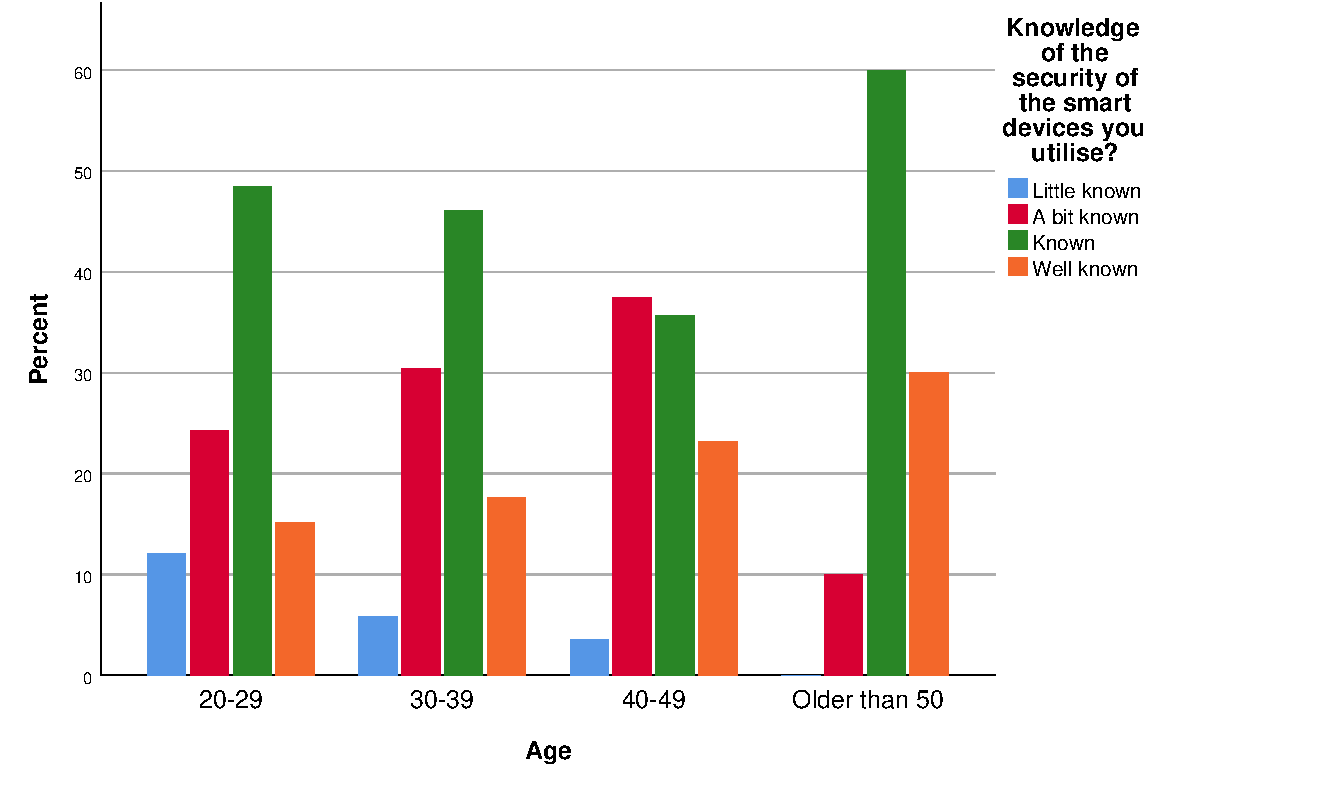
\includegraphics[scale=0.55]{figures/diagrams/age_knowledge-security.pdf}
    \caption{Age differences when it comes to knowledge of smart device security}
    \label{fig:age_knowledge-security}
\end{figure}

\begin{figure}[!h]
    \centering
    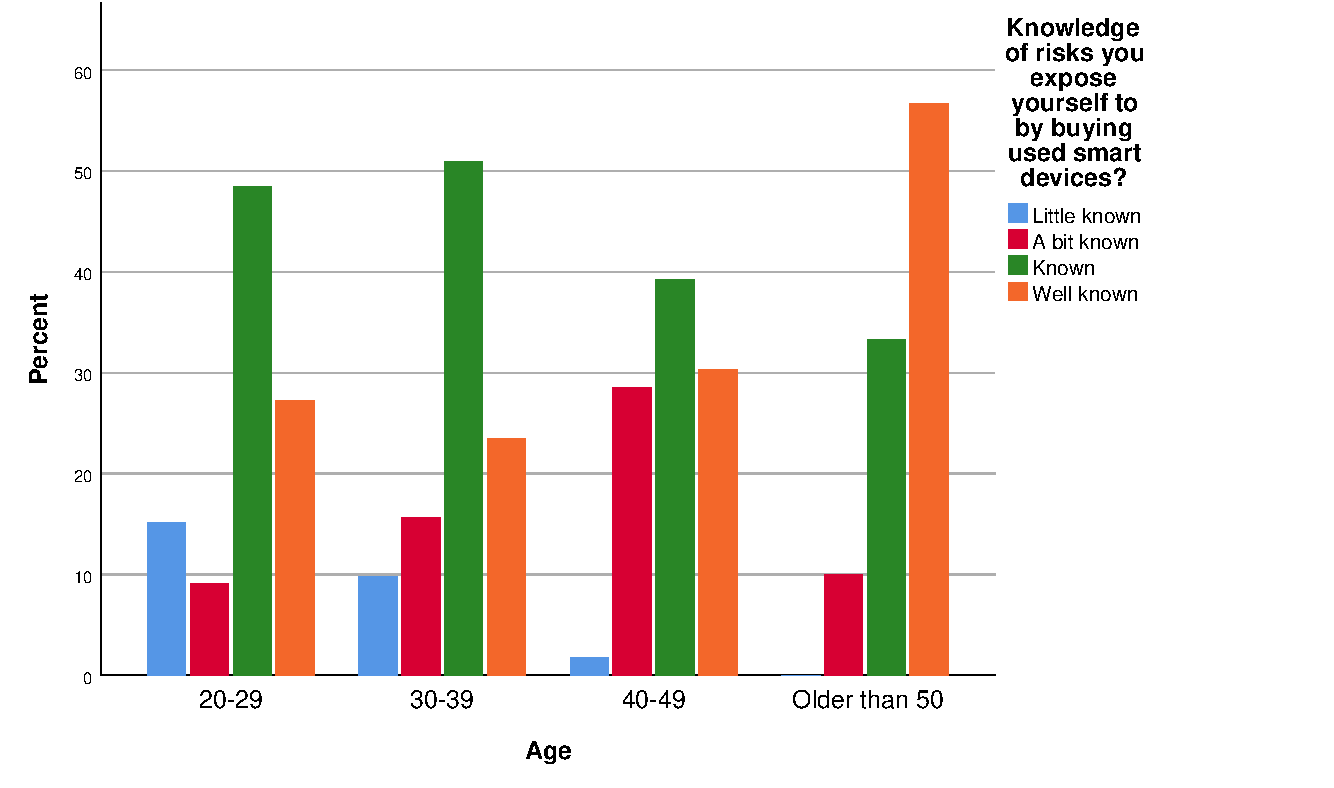
\includegraphics[scale=0.55]{figures/diagrams/age_knowledge-risk.pdf}
    \caption{Age differences when it comes to knowledge of risks by buying used smart devices}
    \label{fig:age_knowledge-risk}
\end{figure}

When it comes to the differences between people who prefer cable or wireless when connecting their smart home devices to the internet, we also see that those older than 50 do significantly more often prefer wireless to cable. This variance is visualised in figure \ref{fig:age_cable-wireless}. 

\begin{figure}[!h]
    \centering
    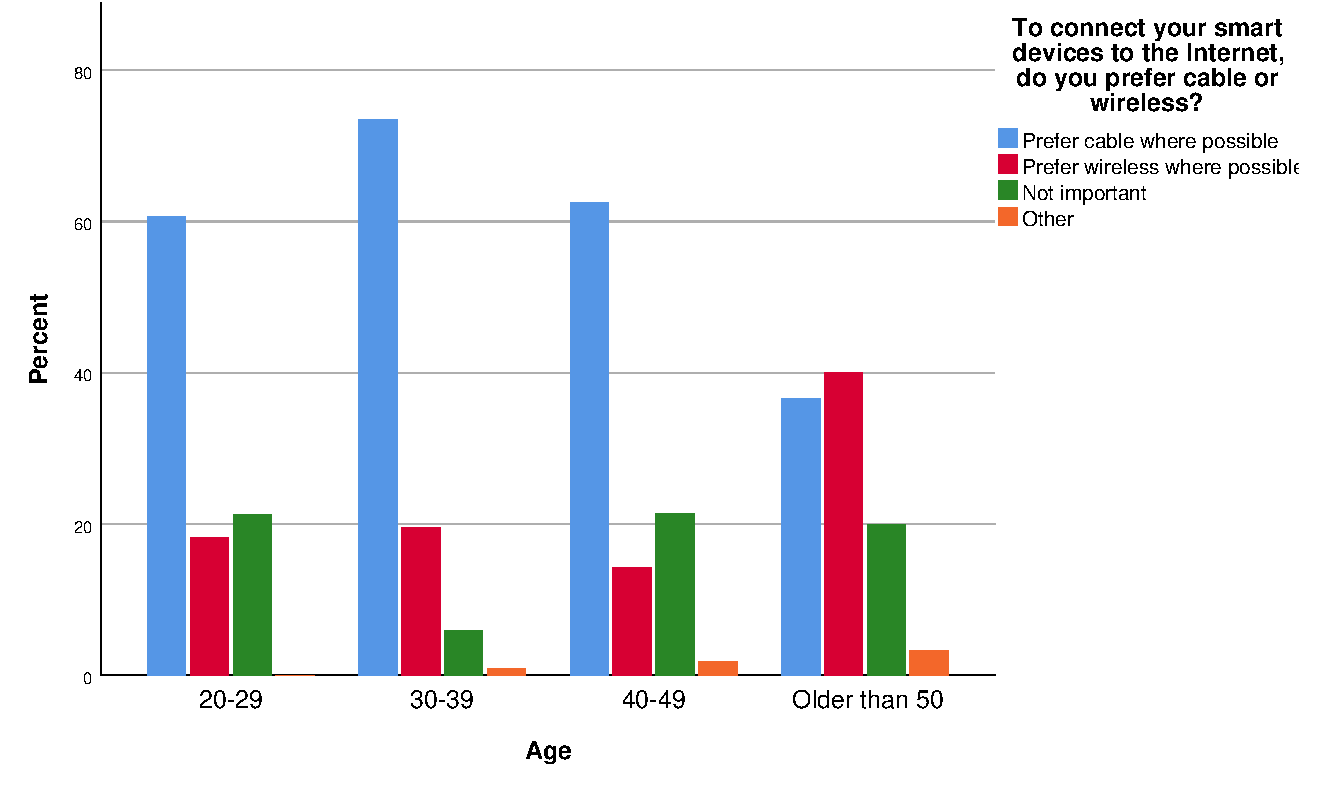
\includegraphics[scale=0.55]{figures/diagrams/age_cable-wireless.pdf}
    \caption{Age differences when preferring cable or wireless to connect to the internet}
    \label{fig:age_cable-wireless}
\end{figure}

\subsection{Education differences}
In the analysis of educational differences, my main findings included variance in whether people used a password manager or not. As is presented in figure \ref{fig:anova_education}, the difference has a significance of 0.028, which means there is only 2.8\% probability that this difference is due to chance alone. This is also under the set threshold of 0.05. 
\begin{figure}[!h]
    \centering
    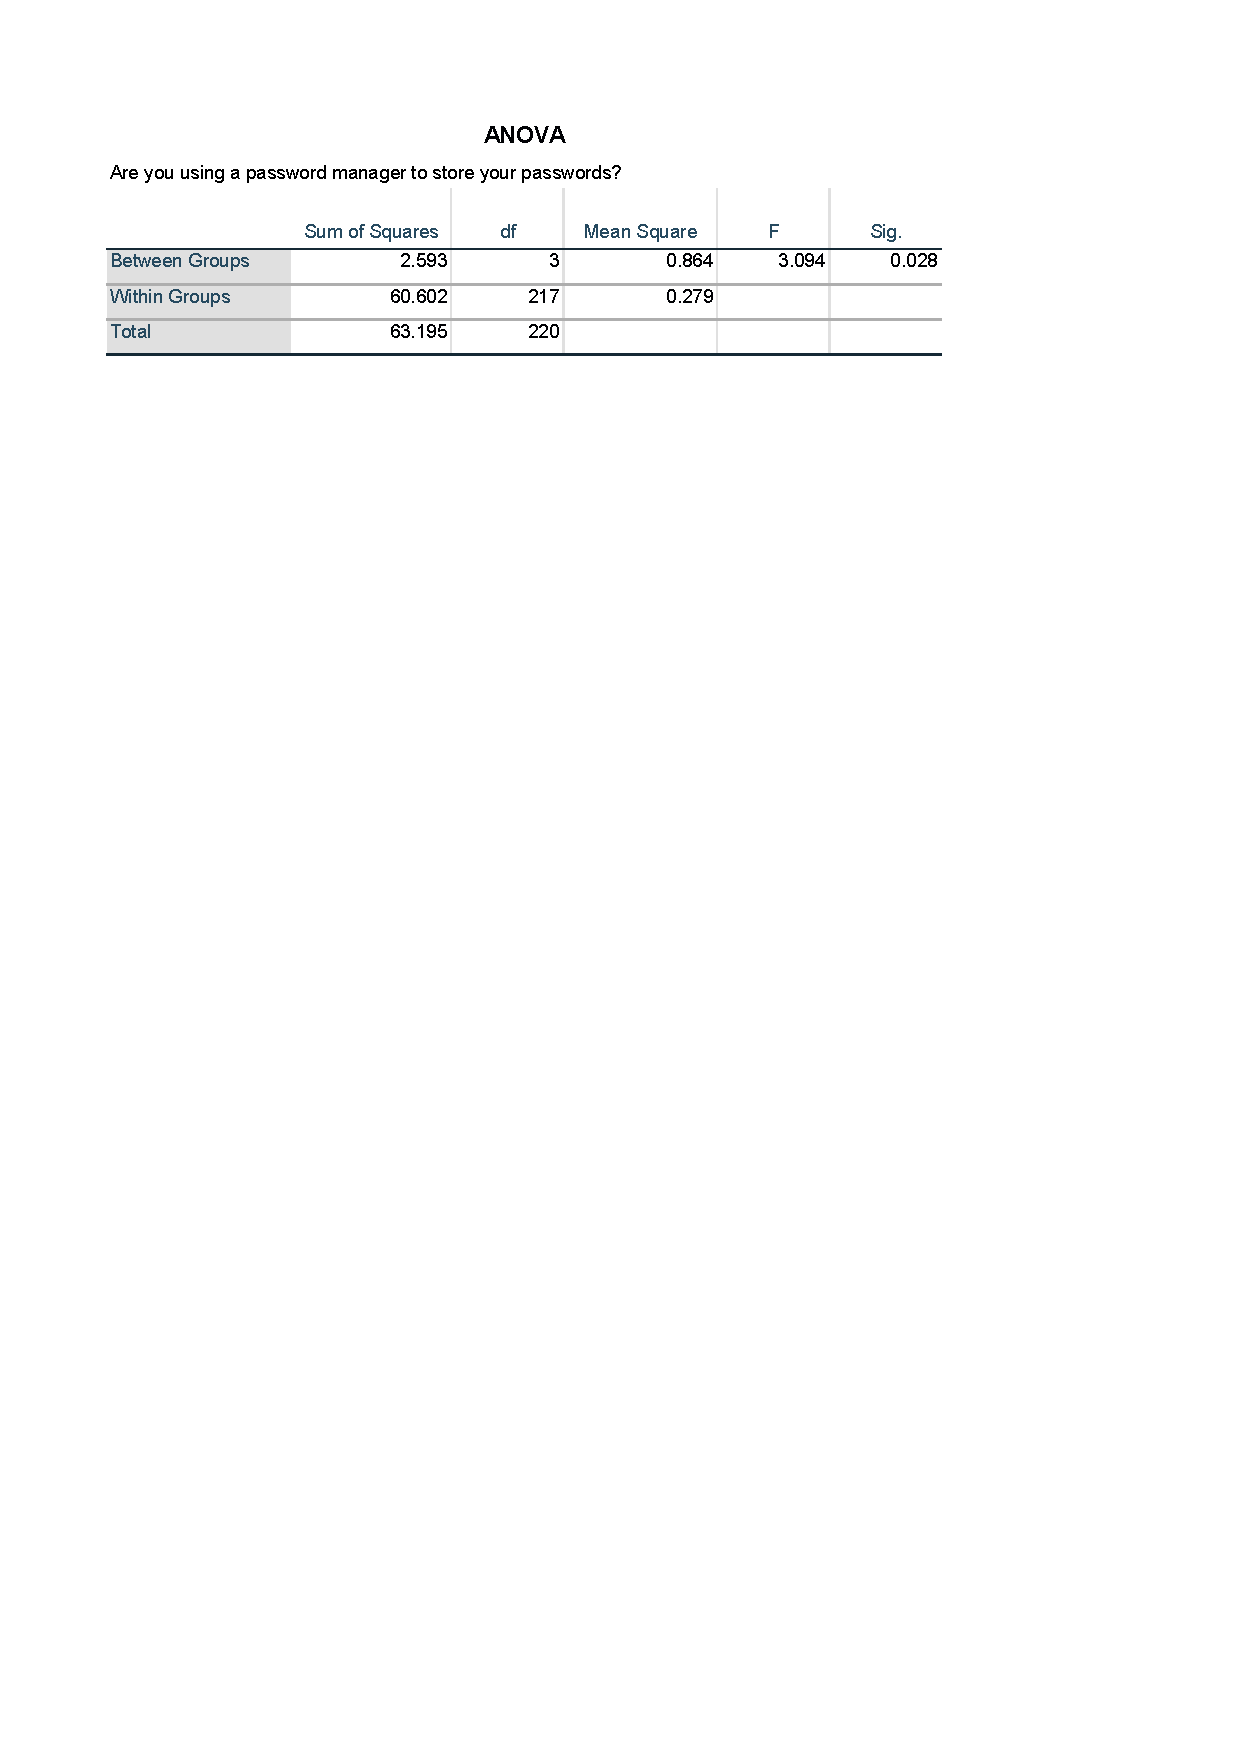
\includegraphics[scale=0.8]{figures/tables/anova_education.pdf}
    \caption{ANOVA of education up against the use of password managers}
    \label{fig:anova_education}
\end{figure}
When looking further at the descriptive statistics in appendix \ref{fig:anova_education_desc}, we see that the mean value is lower for people with university education. As mentioned in the method chapter, yes = 1 and no = 2, so this could mean that university graduates are more likely to answer yes. This difference is further visualised in a bar chart in figure \ref{fig:education_password-manager} below. 

\begin{figure}[!h]
    \centering
    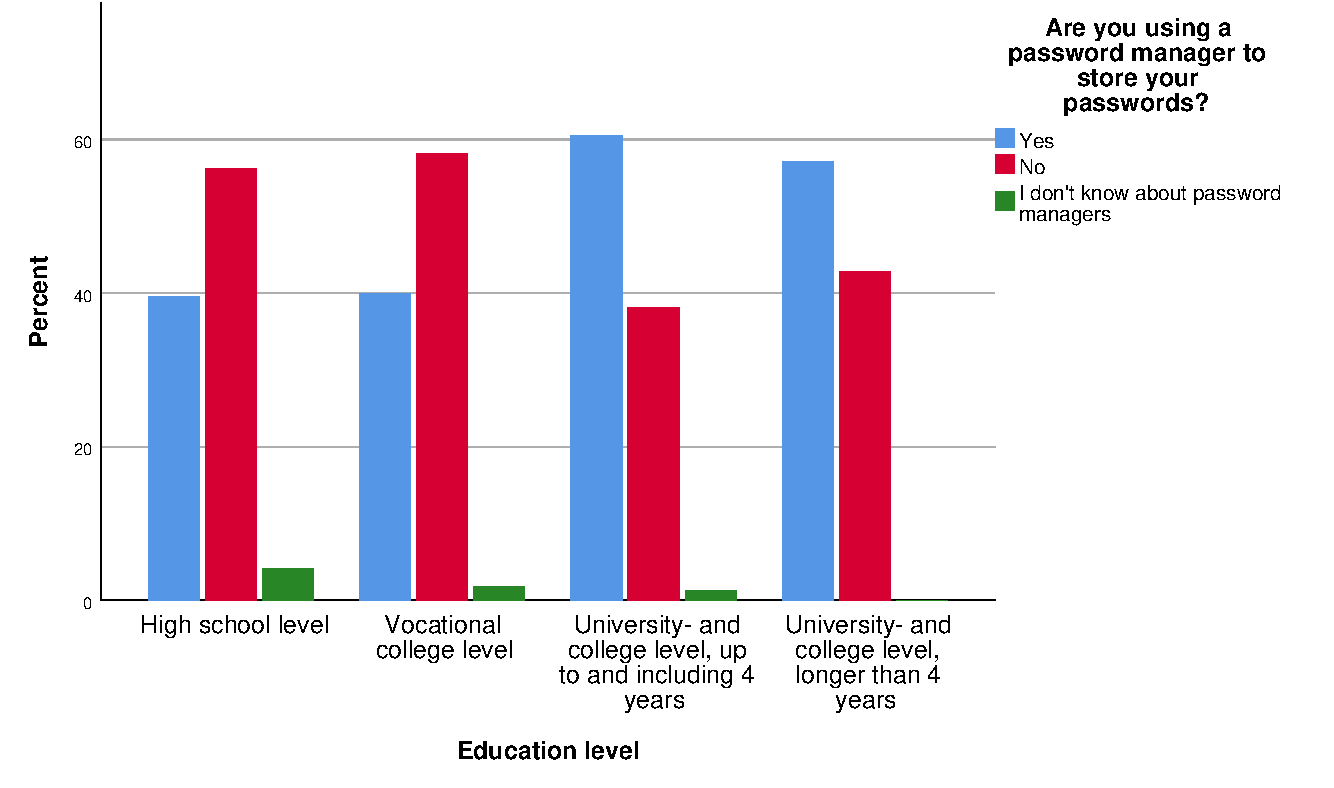
\includegraphics[scale=0.55]{figures/diagrams/education_password-manager.pdf}
    \caption{Education differences when it comes to using password managers}
    \label{fig:education_password-manager}
\end{figure}

When looking at the post-hoc tukey test in appendix \ref{fig:anova_education_tukey}, however, none of the mean differences between the education groups are significantly different. The results should therefore be taken with a grain of salt, even though the ANOVA results show up as significant. 

\subsection{Reasons for changing security and privacy settings}
Back in section \ref{subsec:use_smart_devices} I presented how many people changed the security and privacy settings on their smart home devices. Looking further into this question I wanted to know if those who answered no actually knew about contents of the data they are sending, and if that risk was accepted. I took the independent variable, which was if they changed the security and privacy setting or not, and compared their knowledge of the data flow of their smart devices. The ANOVA in figure \ref{fig:anova_changesettings_dataflow} shows us that there is a difference between the groups of the independent variable that is significant at 0, and that the dependent variable do have an effect on the independent one. 

\begin{figure}[!h]
    \centering
    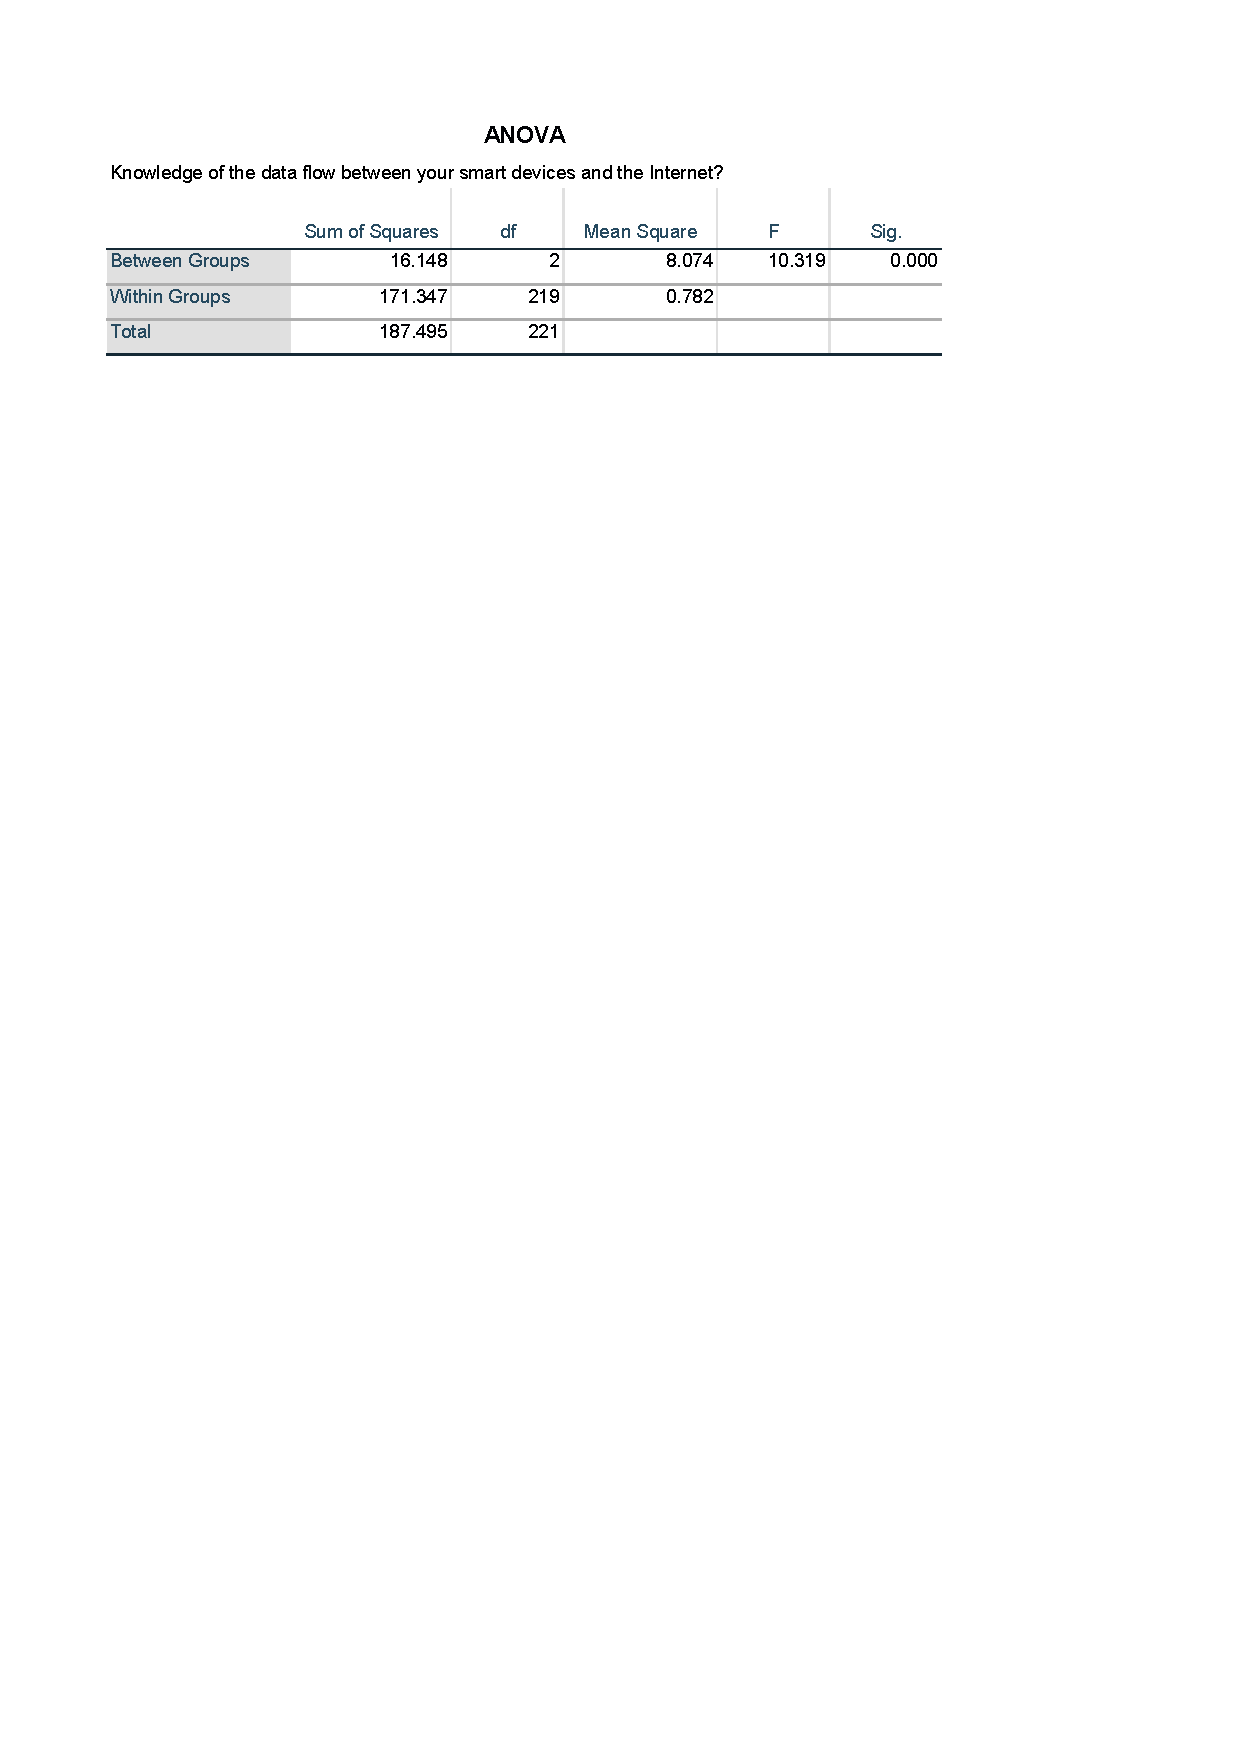
\includegraphics[scale=0.8]{figures/tables/anova_changesettings_dataflow.pdf}
    \caption{ANOVA of whether knowledge of data flow affects changing security and privacy settings}
    \label{fig:anova_changesettings_dataflow}
\end{figure}
When we look at the descriptive statistics in appendix \ref{fig:anova_changesettings_dataflow_desc}, we see that the mean value of data flow knowledge for those who said yes to changing their settings is at 3.06, while it is 2.55 for those who said no. When looking at the post-hoc tukey test, in appendix \ref{fig:anova_changesettings_dataflow_tukey}, we see that the mean difference between saying yes or no is 0.517, which is also significant at the 0.05 level. This difference is further visualised in the bar chart \ref{fig:changesetting_dataflow} below. 

\begin{figure}[!h]
    \centering
    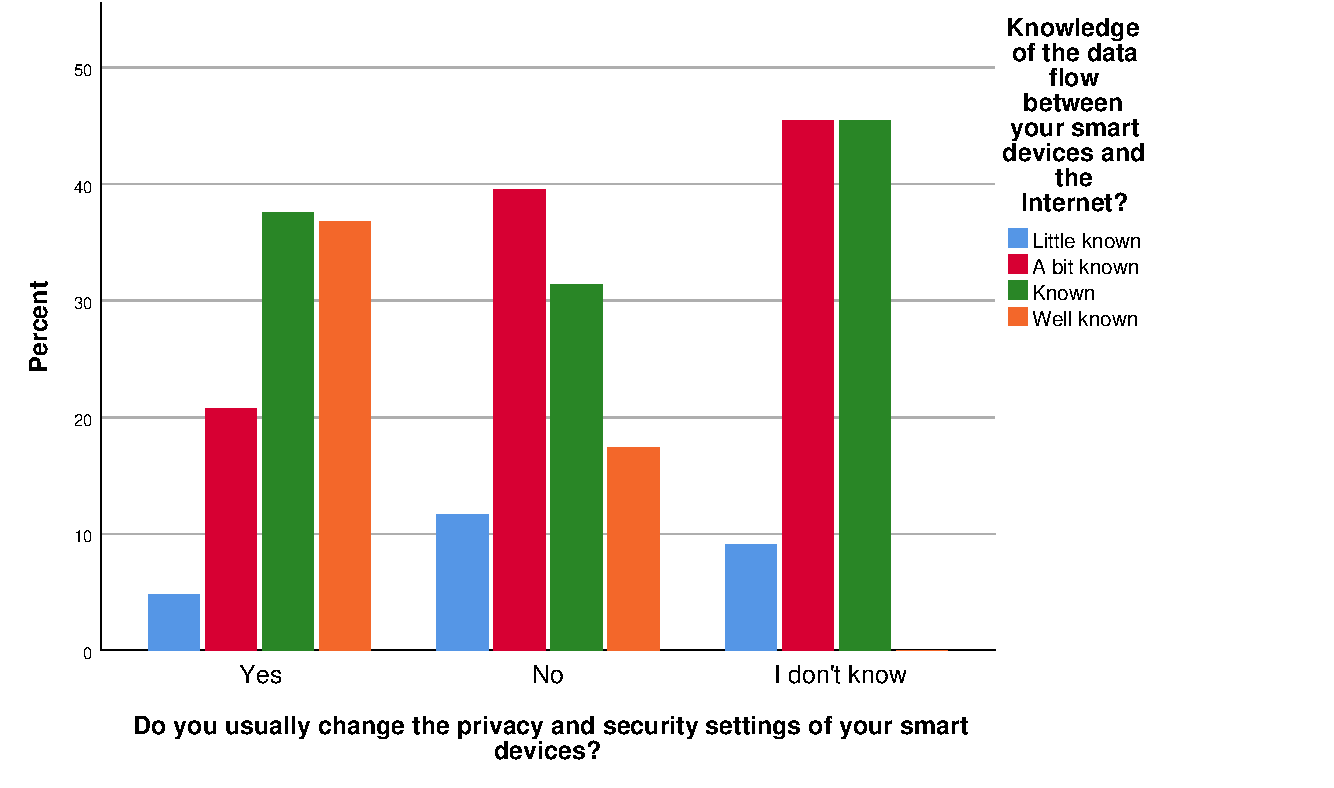
\includegraphics[scale=0.55]{figures/diagrams/changesettings_dataflow.pdf}
    \caption{ANOVA of whether knowledge of data flow affects changing security and privacy settings}
    \label{fig:changesetting_dataflow}
\end{figure}

\section{Control group analysis}
In this section I will go over the findings of my control group analysis. The number of respondents for the control group was 43 people. 

\subsection{Demographics}
Before presenting the results, I will describe the control group sample demographics and compare it to the main sample. 

\subsubsection{Age}
A visual representation of the age distribution and comparison to the main sample is included in figure \ref{fig:age_controlgroup} below. 
\begin{figure}[!h]
    \centering
    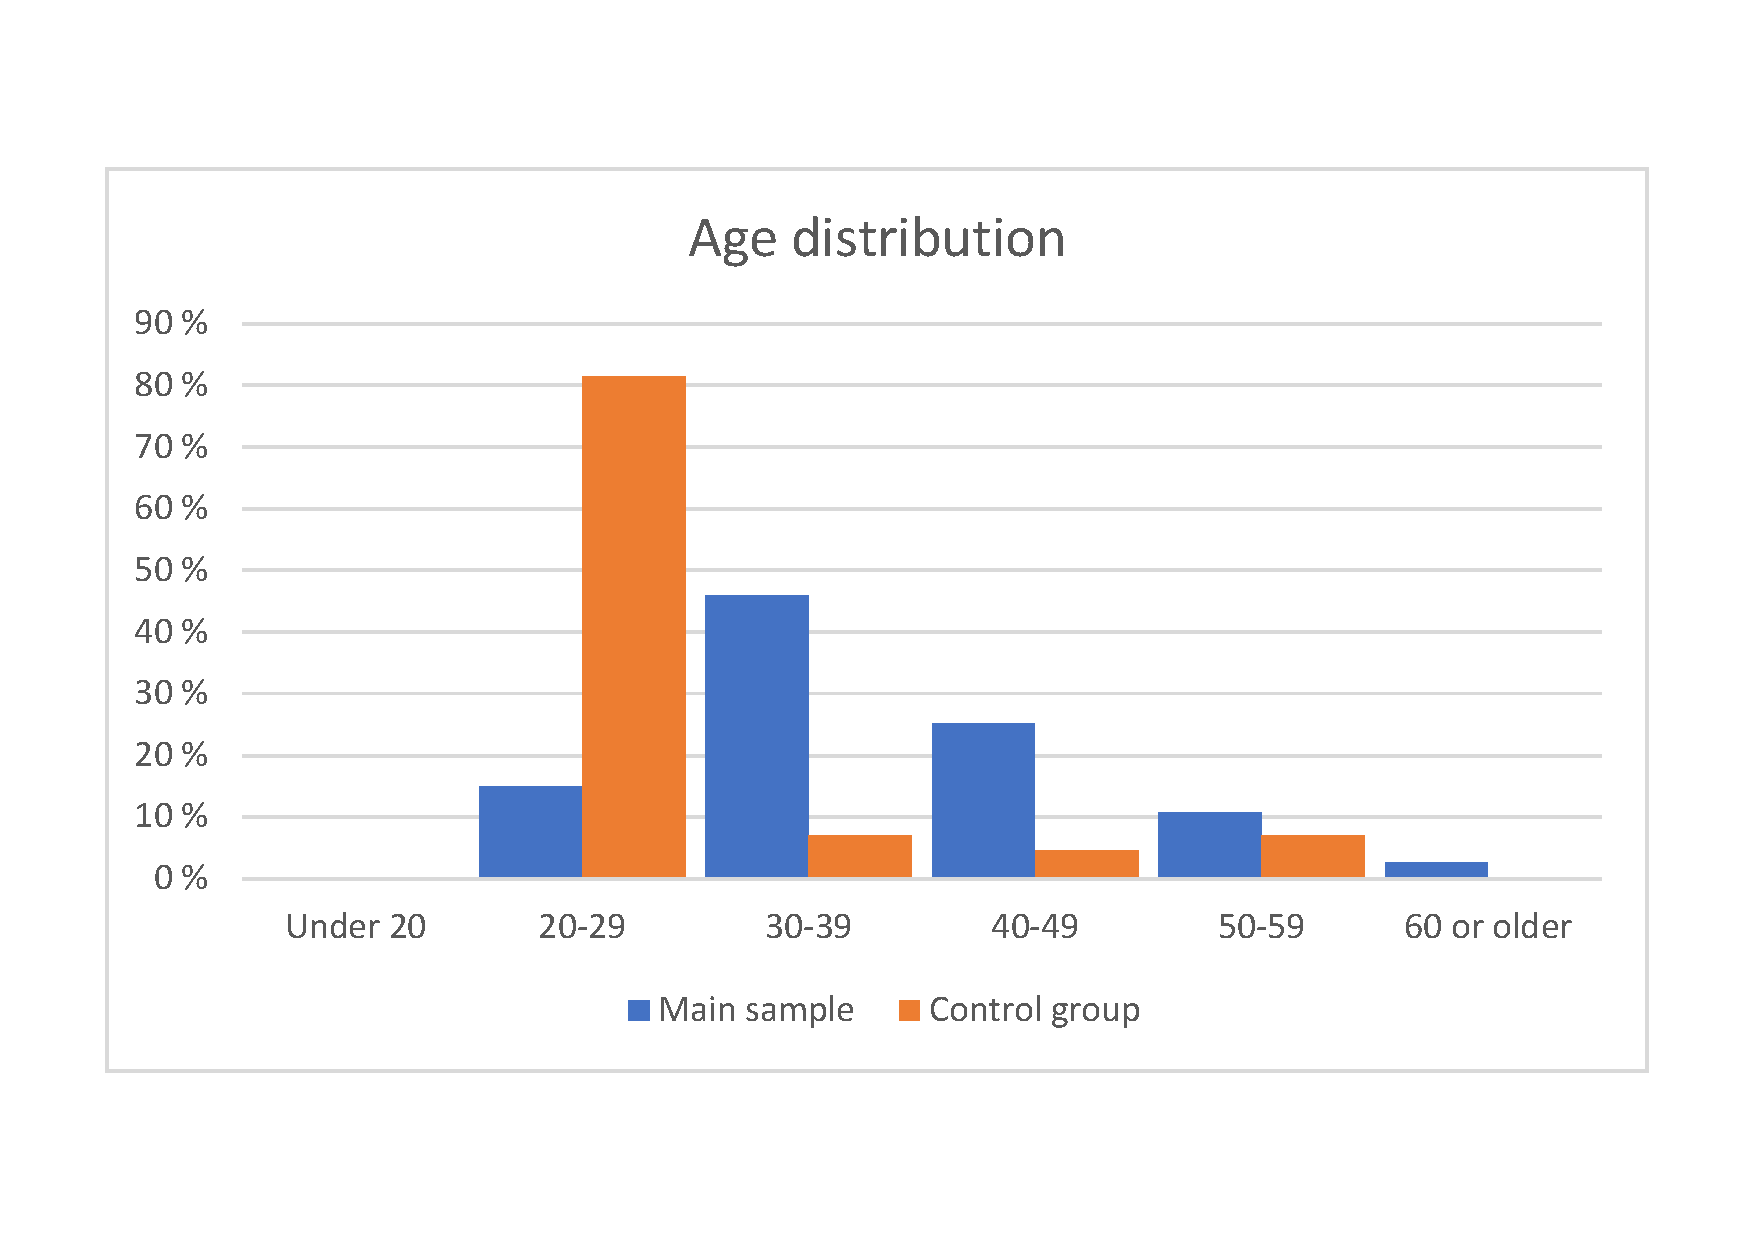
\includegraphics[scale=0.40]{figures/diagrams/age_controlgroup.pdf}
    \caption{Age distribution of the control group in comparison with the main sample}
    \label{fig:age_controlgroup}
\end{figure}
In the control group sample, a total of 35 people (81.4\%) respondent to being between 20 and 29 years old. This means that the control group is overwhelmingly made up of young people, especially compared to the main sample. 

\subsubsection{Gender}
When it comes to the gender distribution, it seems much closer to 50/50, especially in comparison to the main sample, which had all males expect for one person who preferred not answering. The distribution is shown in figure \ref{fig:gender_controlgroup} below. 
\begin{figure}[!h]
    \centering
    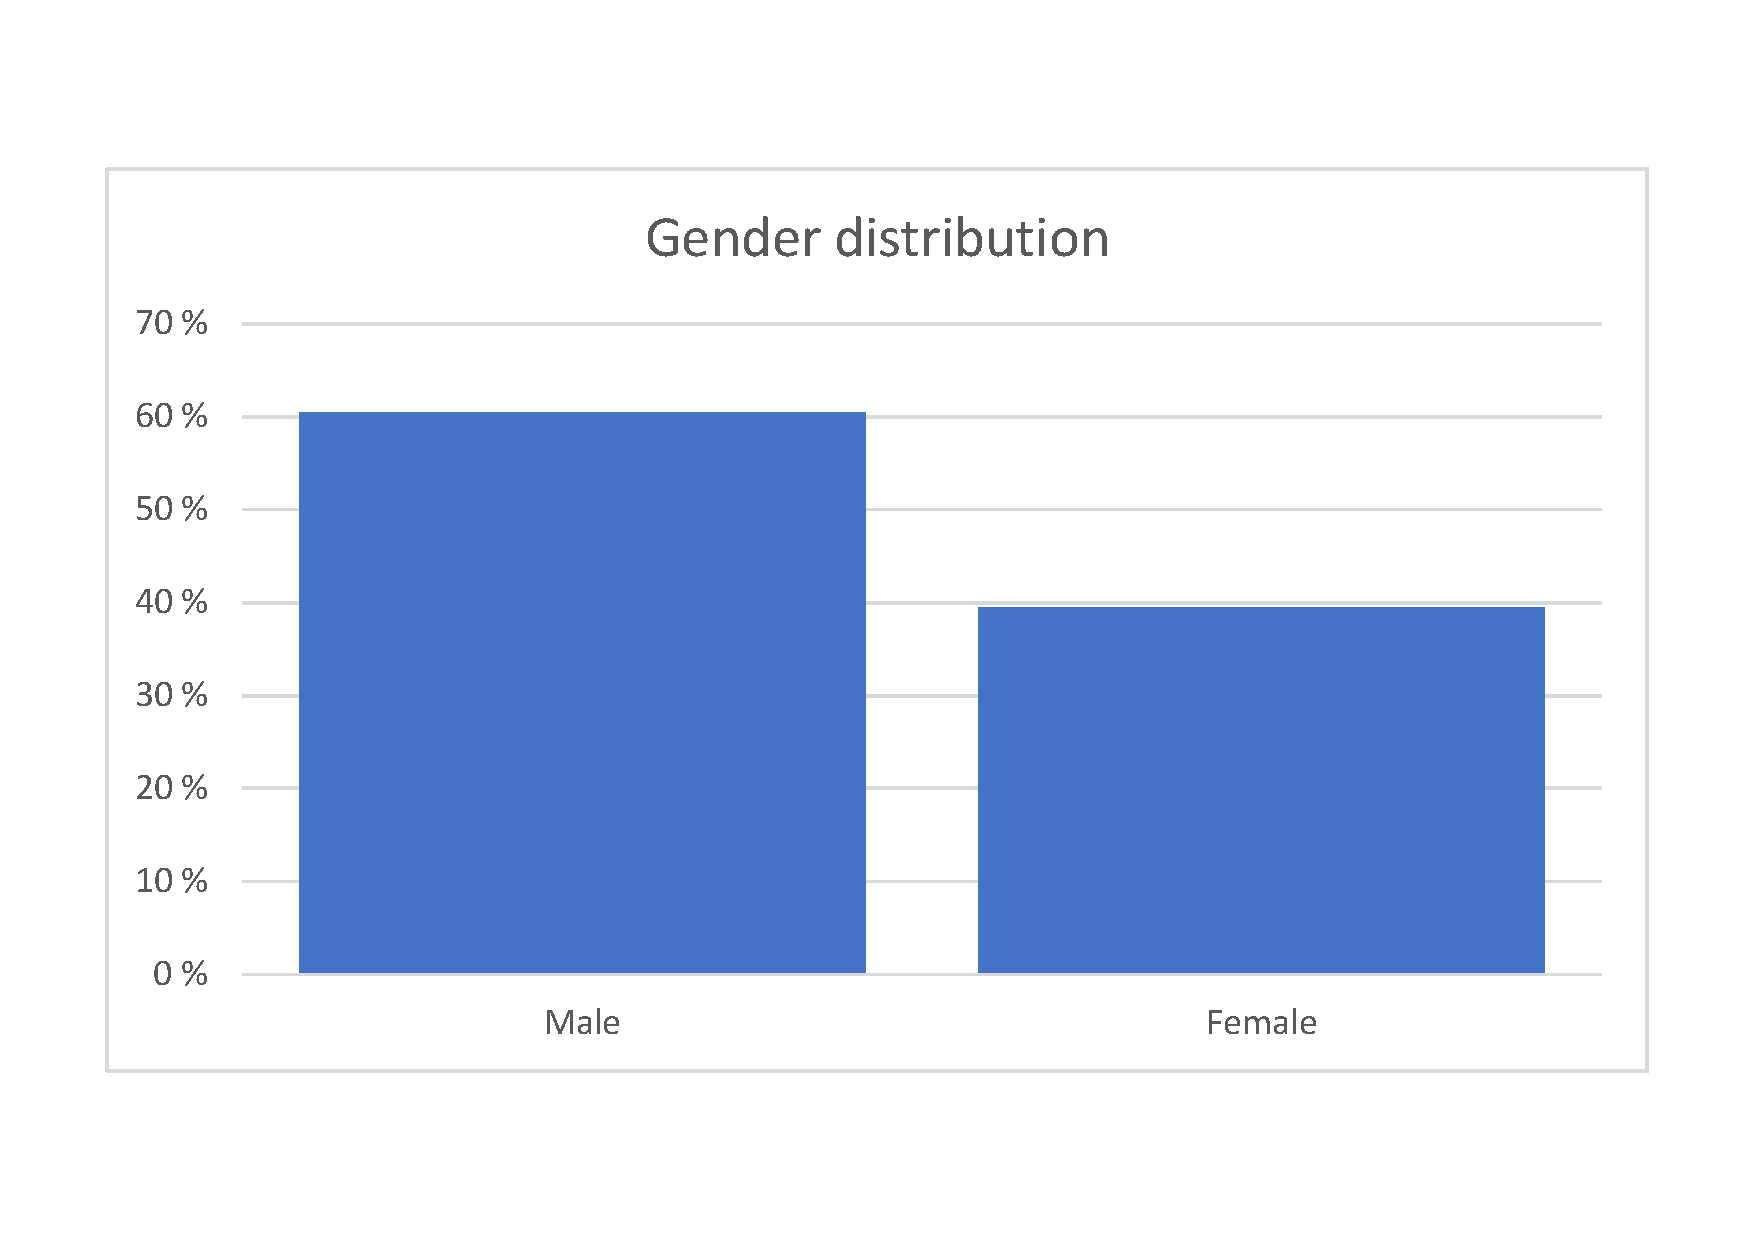
\includegraphics[scale=0.40]{figures/diagrams/gender_controlgroup.pdf}
    \caption{Gender distribution of the control group}
    \label{fig:gender_controlgroup}
\end{figure}
In this sample, 26 people (60.5\%) responded that they were male, while 17 people (39.5\%) said they were female. This is much closer to the national average than the main sample. 

\subsubsection{Highest education level}
Regarding education level both similarities and differences are observed. As we can see in figure \ref{fig:education_controlgroup} below, there is about the same share of people with high school education and slightly more people with higher education. The big difference, however, is the people who answered to having vocational college education. 
\begin{figure}[!h]
    \centering
    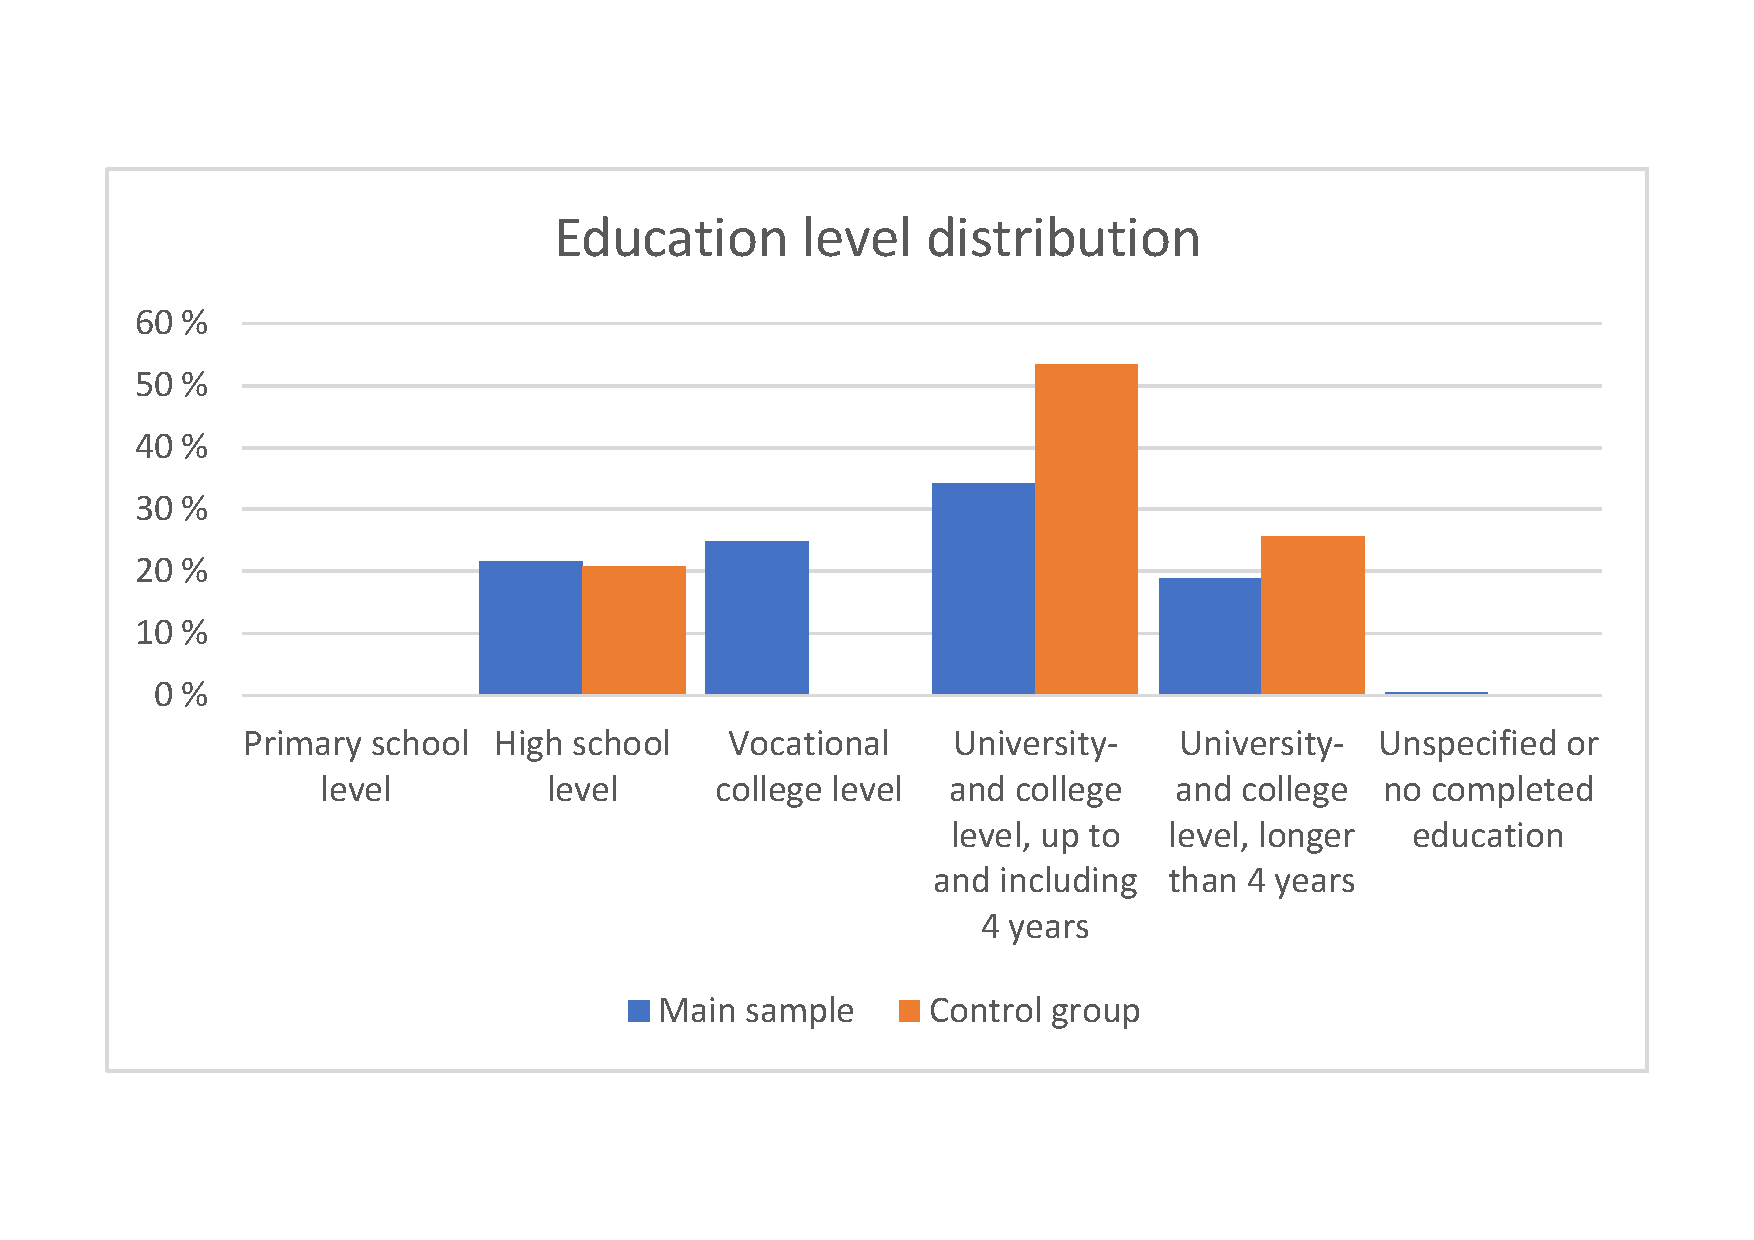
\includegraphics[scale=0.40]{figures/diagrams/education_controlgroup.pdf}
    \caption{Highest completed education level of the control group}
    \label{fig:education_controlgroup}
\end{figure}
In the control group sample, none of the respondents had vocational college education, while it amounted to about a quarter of the respondents in the main sample. 

\subsubsection{County}
The county population distribution of the control group is visualised in figure \ref{fig:county_controlgroup} below. Compared to the main sample it seems to have much more people from Innlandet county. About 30\% responded to living in Innlandet, compared to 5\% in my main sample, and 7\% nationally. 
\begin{figure}[!h]
    \centering
    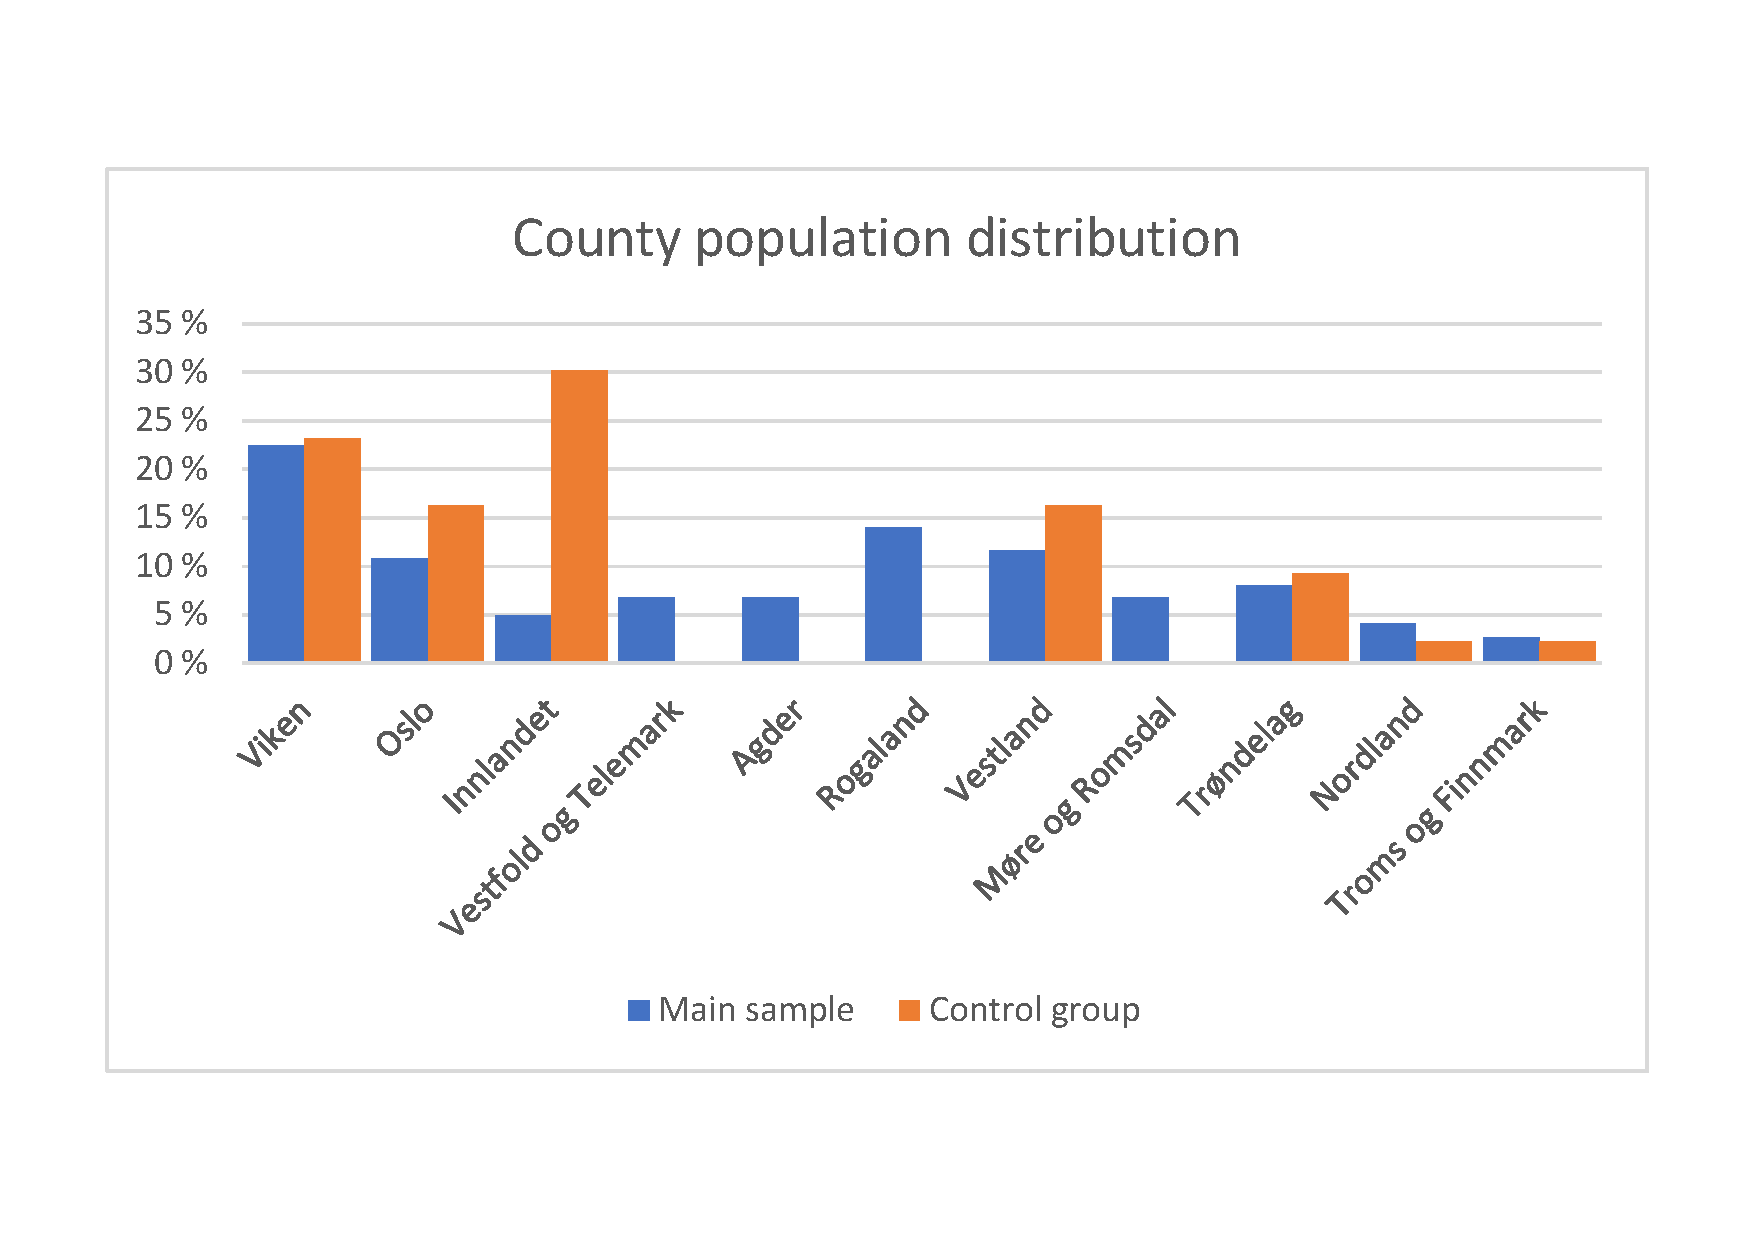
\includegraphics[scale=0.40]{figures/diagrams/county_controlgroup.pdf}
    \caption{County population distribution of the control group}
    \label{fig:county_controlgroup}
\end{figure}
Due to the low sample size and high number of possible answers these results may not be very representative, as some categories does not even have a single answer. 

\subsection{Analysis of differences to the main sample}
To start off, in order to make the control group sample available to more people than just smart home owners, I included an additional question where I asked if they owned any smart devices. The results from this question can be seen in figure \ref{fig:controlgroup_ownsmartdevice} below. 
\begin{figure}[!h]
    \centering
    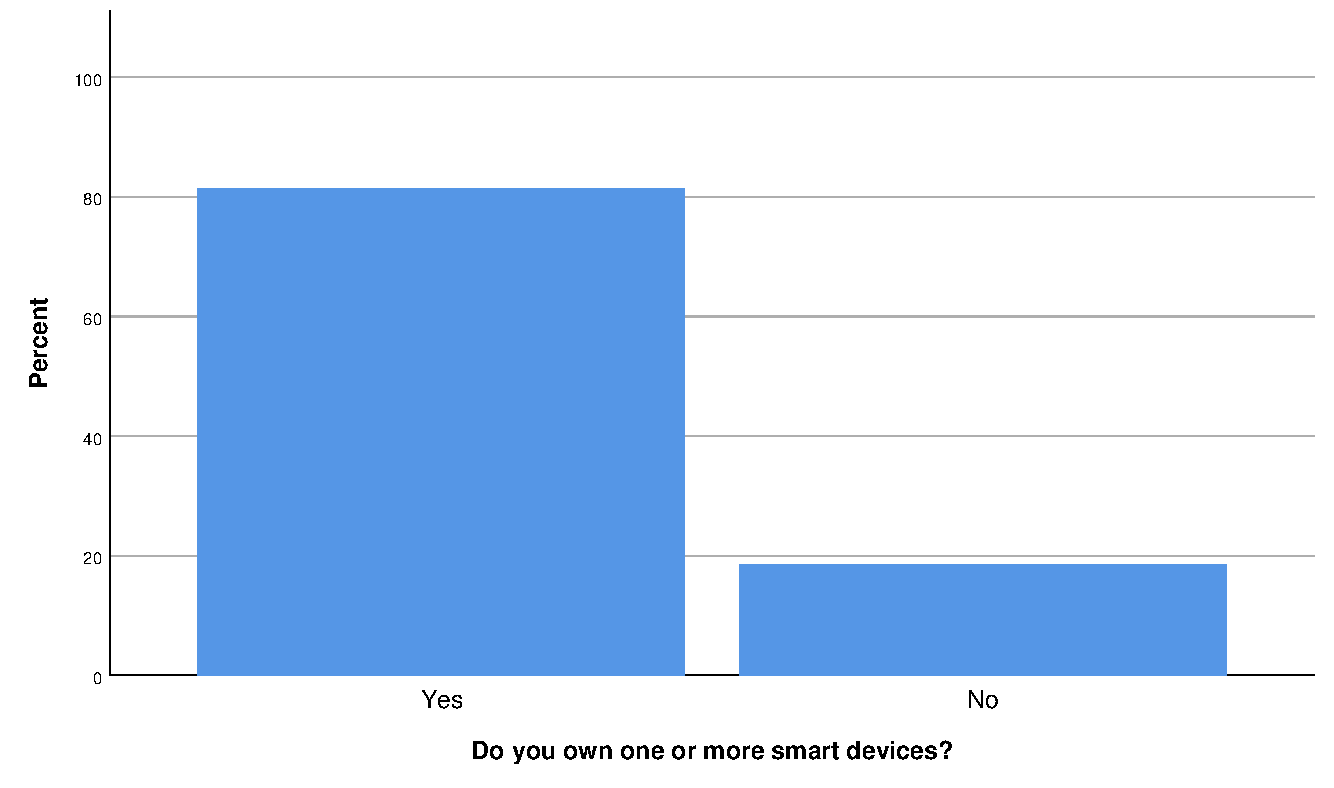
\includegraphics[scale=0.55]{figures/diagrams/controlgroup_ownsmartdevice.pdf}
    \caption{The part of the sample who reported to owning one or more smart devices}
    \label{fig:controlgroup_ownsmartdevice}
\end{figure}
Out of the 43 total respondents, 35 people (81.4\%) answered that they owned smart devices, while 8 people (18.6\%) did not. Those who answered yes received additional questions regarding smart home devices, compared to the ones who answered no. 

\textcolor{red}{Possibly move to limitations in discussion?}
In retrospect, I realised I should have specified smart home devices, and not just smart devices, since it may be people who misinterpret the question to include regular smart phones or other devices. Therefore, the percentage of people owning smart home devices could be lower than the displayed results. 

\subsubsection{Differences in smart device types owned}
For those 35 people who said they owned smart devices, I asked what types of smart devices they owned. In table \ref{tab:controlgroup_howsmart_N} below is an overview of the number of respondents that answered this question. 
\begin{table}[!h]
\centering
\begin{tabular}{|l|c|c|c|c|c|c|}
\hline
\multicolumn{7}{|c|}{{\color[HTML]{010205} \textbf{Case Summary}}} \\ \hline
{\color[HTML]{264A60} } &
  \multicolumn{6}{c|}{{\color[HTML]{264A60} Cases}} \\ \cline{2-7} 
{\color[HTML]{264A60} } &
  \multicolumn{2}{c|}{{\color[HTML]{264A60} Valid}} &
  \multicolumn{2}{c|}{{\color[HTML]{264A60} Missing}} &
  \multicolumn{2}{c|}{{\color[HTML]{264A60} Total}} \\ \cline{2-7} 
\multirow{-3}{*}{{\color[HTML]{264A60} }} &
  {\color[HTML]{264A60} N} &
  {\color[HTML]{264A60} Percent} &
  {\color[HTML]{264A60} N} &
  {\color[HTML]{264A60} Percent} &
  {\color[HTML]{264A60} N} &
  {\color[HTML]{264A60} Percent} \\ \hline
\cellcolor[HTML]{E0E0E0}{\color[HTML]{264A60} Smart devices} &
  \multicolumn{1}{r|}{{\color[HTML]{010205} 34}} &
  \multicolumn{1}{r|}{{\color[HTML]{010205} 79.1\%}} &
  \multicolumn{1}{r|}{{\color[HTML]{010205} 9}} &
  \multicolumn{1}{r|}{{\color[HTML]{010205} 20.9\%}} &
  \multicolumn{1}{r|}{{\color[HTML]{010205} 43}} &
  \multicolumn{1}{r|}{{\color[HTML]{010205} 100.0\%}} \\ \hline
\end{tabular}
\caption{Number of people in the control group who specified what smart device types they own}
\label{tab:controlgroup_howsmart_N}
\end{table}
Out of the 9 cases that were missing, 8 of them did not receive the question due to now owning smart devices as described in the previous section. The last person did not specify any device types, however he described in freetext that he owned a smart phone and tablet. This confirms that at least one person misunderstood the definition. 
Table \ref{tab:controlgroup_howsmart} below shows us the frequencies of different smart device types people own. 
\begin{table}[!h]
\centering
\begin{tabular}{|c|l|r|r|r|}
\hline
\multicolumn{5}{|c|}{{\color[HTML]{010205} \textbf{Smart device types frequencies}}} \\ \hline
\multicolumn{2}{|l|}{{\color[HTML]{264A60} }} &
  \multicolumn{2}{c|}{{\color[HTML]{264A60} Responses}} &
  \multicolumn{1}{c|}{{\color[HTML]{264A60} }} \\ \cline{3-4}
\multicolumn{2}{|l|}{\multirow{-2}{*}{{\color[HTML]{264A60} }}} &
  \multicolumn{1}{c|}{{\color[HTML]{264A60} N}} &
  \multicolumn{1}{c|}{{\color[HTML]{264A60} Percent}} &
  \multicolumn{1}{c|}{\multirow{-2}{*}{{\color[HTML]{264A60} Percent of Cases}}} \\ \hline
\cellcolor[HTML]{E0E0E0}{\color[HTML]{264A60} } &
  \cellcolor[HTML]{E0E0E0}{\color[HTML]{264A60} Voice assistant} &
  {\color[HTML]{010205} 8} &
  {\color[HTML]{010205} 6.8\%} &
  {\color[HTML]{010205} 23.5\%} \\ \cline{2-5} 
\cellcolor[HTML]{E0E0E0}{\color[HTML]{264A60} } &
  \cellcolor[HTML]{E0E0E0}{\color[HTML]{264A60} Speaker} &
  {\color[HTML]{010205} 20} &
  {\color[HTML]{010205} 17.1\%} &
  {\color[HTML]{010205} 58.8\%} \\ \cline{2-5} 
\cellcolor[HTML]{E0E0E0}{\color[HTML]{264A60} } &
  \cellcolor[HTML]{E0E0E0}{\color[HTML]{264A60} Robot vacuum} &
  {\color[HTML]{010205} 9} &
  {\color[HTML]{010205} 7.7\%} &
  {\color[HTML]{010205} 26.5\%} \\ \cline{2-5} 
\cellcolor[HTML]{E0E0E0}{\color[HTML]{264A60} } &
  \cellcolor[HTML]{E0E0E0}{\color[HTML]{264A60} Smarthub} &
  {\color[HTML]{010205} 1} &
  {\color[HTML]{010205} 0.9\%} &
  {\color[HTML]{010205} 2.9\%} \\ \cline{2-5} 
\cellcolor[HTML]{E0E0E0}{\color[HTML]{264A60} } &
  \cellcolor[HTML]{E0E0E0}{\color[HTML]{264A60} Smart TV} &
  {\color[HTML]{010205} 21} &
  {\color[HTML]{010205} 17.9\%} &
  {\color[HTML]{010205} 61.8\%} \\ \cline{2-5} 
\cellcolor[HTML]{E0E0E0}{\color[HTML]{264A60} } &
  \cellcolor[HTML]{E0E0E0}{\color[HTML]{264A60} Smart screen} &
  {\color[HTML]{010205} 2} &
  {\color[HTML]{010205} 1.7\%} &
  {\color[HTML]{010205} 5.9\%} \\ \cline{2-5} 
\cellcolor[HTML]{E0E0E0}{\color[HTML]{264A60} } &
  \cellcolor[HTML]{E0E0E0}{\color[HTML]{264A60} Router} &
  {\color[HTML]{010205} 16} &
  {\color[HTML]{010205} 13.7\%} &
  {\color[HTML]{010205} 47.1\%} \\ \cline{2-5} 
\cellcolor[HTML]{E0E0E0}{\color[HTML]{264A60} } &
  \cellcolor[HTML]{E0E0E0}{\color[HTML]{264A60} Door lock} &
  {\color[HTML]{010205} 4} &
  {\color[HTML]{010205} 3.4\%} &
  {\color[HTML]{010205} 11.8\%} \\ \cline{2-5} 
\cellcolor[HTML]{E0E0E0}{\color[HTML]{264A60} } &
  \cellcolor[HTML]{E0E0E0}{\color[HTML]{264A60} Light bulbs} &
  {\color[HTML]{010205} 7} &
  {\color[HTML]{010205} 6.0\%} &
  {\color[HTML]{010205} 20.6\%} \\ \cline{2-5} 
\cellcolor[HTML]{E0E0E0}{\color[HTML]{264A60} } &
  \cellcolor[HTML]{E0E0E0}{\color[HTML]{264A60} Smart dimmer} &
  {\color[HTML]{010205} 6} &
  {\color[HTML]{010205} 5.1\%} &
  {\color[HTML]{010205} 17.6\%} \\ \cline{2-5} 
\cellcolor[HTML]{E0E0E0}{\color[HTML]{264A60} } &
  \cellcolor[HTML]{E0E0E0}{\color[HTML]{264A60} Smart switch} &
  {\color[HTML]{010205} 4} &
  {\color[HTML]{010205} 3.4\%} &
  {\color[HTML]{010205} 11.8\%} \\ \cline{2-5} 
\cellcolor[HTML]{E0E0E0}{\color[HTML]{264A60} } &
  \cellcolor[HTML]{E0E0E0}{\color[HTML]{264A60} Kitchenware} &
  {\color[HTML]{010205} 5} &
  {\color[HTML]{010205} 4.3\%} &
  {\color[HTML]{010205} 14.7\%} \\ \cline{2-5} 
\cellcolor[HTML]{E0E0E0}{\color[HTML]{264A60} } &
  \cellcolor[HTML]{E0E0E0}{\color[HTML]{264A60} Alarms} &
  {\color[HTML]{010205} 5} &
  {\color[HTML]{010205} 4.3\%} &
  {\color[HTML]{010205} 14.7\%} \\ \cline{2-5} 
\cellcolor[HTML]{E0E0E0}{\color[HTML]{264A60} } &
  \cellcolor[HTML]{E0E0E0}{\color[HTML]{264A60} Motion sensors} &
  {\color[HTML]{010205} 3} &
  {\color[HTML]{010205} 2.6\%} &
  {\color[HTML]{010205} 8.8\%} \\ \cline{2-5} 
\multirow{-15}{*}{\cellcolor[HTML]{E0E0E0}{\color[HTML]{264A60} Smart devices}} &
  \cellcolor[HTML]{E0E0E0}{\color[HTML]{264A60} Thermostat} &
  {\color[HTML]{010205} 6} &
  {\color[HTML]{010205} 5.1\%} &
  {\color[HTML]{010205} 17.6\%} \\ \hline
\multicolumn{2}{|l|}{\cellcolor[HTML]{E0E0E0}{\color[HTML]{264A60} Total}} &
  {\color[HTML]{010205} 117} &
  {\color[HTML]{010205} 100.0\%} &
  {\color[HTML]{010205} 344.1\%} \\ \hline
\end{tabular}
\caption{What types of smart devices the respondents in the control group own}
\label{tab:controlgroup_howsmart}
\end{table}
We can see that the total number of responses is 117 since people can make multiple choices. Considering there were 34 poeple who answered, this means that on average people only chose between three and four device types each. The three most popular device types were smart speakers (58.8\% of the time), smart TV's (61.8\% of the time), and routers (47.1\% of the time). The answers shows us that most people in this control sample have much more basic smart homes with much fewer device types than in our main sample. People in the main sample had on average a little over ten device types, and maybe even more if we consider freetext answers. Speaking of freetext answers, one person in the control group sample also specified that they owned a robot lawn mower, and one person said they had a smart washing machine. 

\subsection{Differences in knowledge of certain topics and aspects}
Another aspect in which I received results that were different from the main sample was when assessing the respondents knowledge of certain security issues regarding smart devices and knowledge of technology, data security, and smart homes. The results are shown in a stacked bar chart in figure \ref{fig:controlgroup_knowledge} below. 
\begin{figure}[!h]
    \centering
    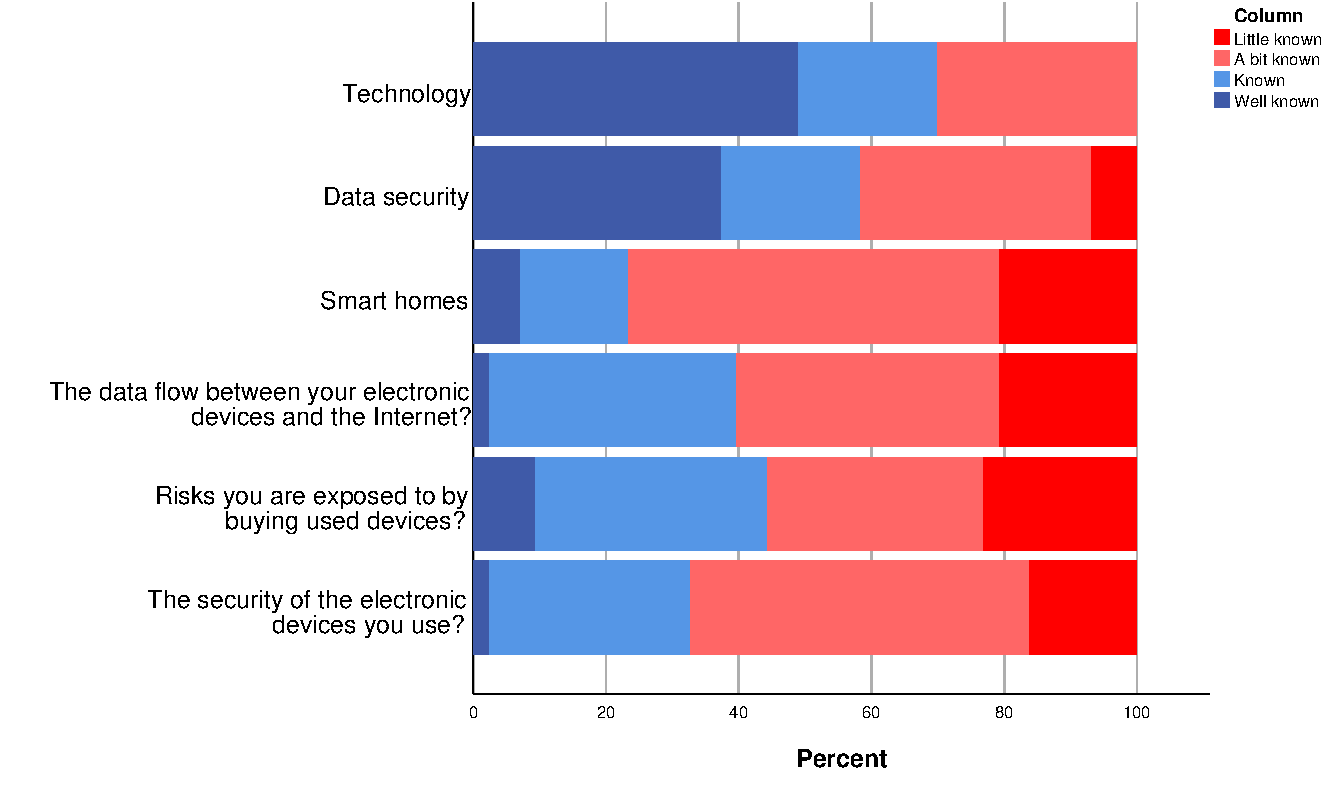
\includegraphics[scale=0.55]{figures/diagrams/controlgroup_knowledge.pdf}
    \caption{The knowledge of the control group respondents regarding different topics}
    \label{fig:controlgroup_knowledge}
\end{figure}
In the last three questions the word smart devices is exchanged with electronic devices to make people with no smart home devices able to answer, while still retaining the same aspect that is analysed. When comparing the results to the main sample in figure \ref{fig:knowledge} and \ref{fig:knowledge_security}, we see that on average the control group reports overall lower knowledge in every of the six aspects. 
\subsubsection{Differences in use of devices}
When comparing the two samples I found some interesting differences in device usage. When analysing the question about if their smart devices was on a separate segment of their home network, I saw that only 6 people (17.1\%) that answered this question from the control group used a separate segment, compared to 41\% from the main sample. Also, 7 people (20\%) said they did not know, compared to 0.5\% from the main sample. The ones who said no were fairly similar in size for both samples. The results is visualised and compared in figure \ref{fig:controlgroup_separatesegment} below.
\begin{figure}[!h]
    \centering
    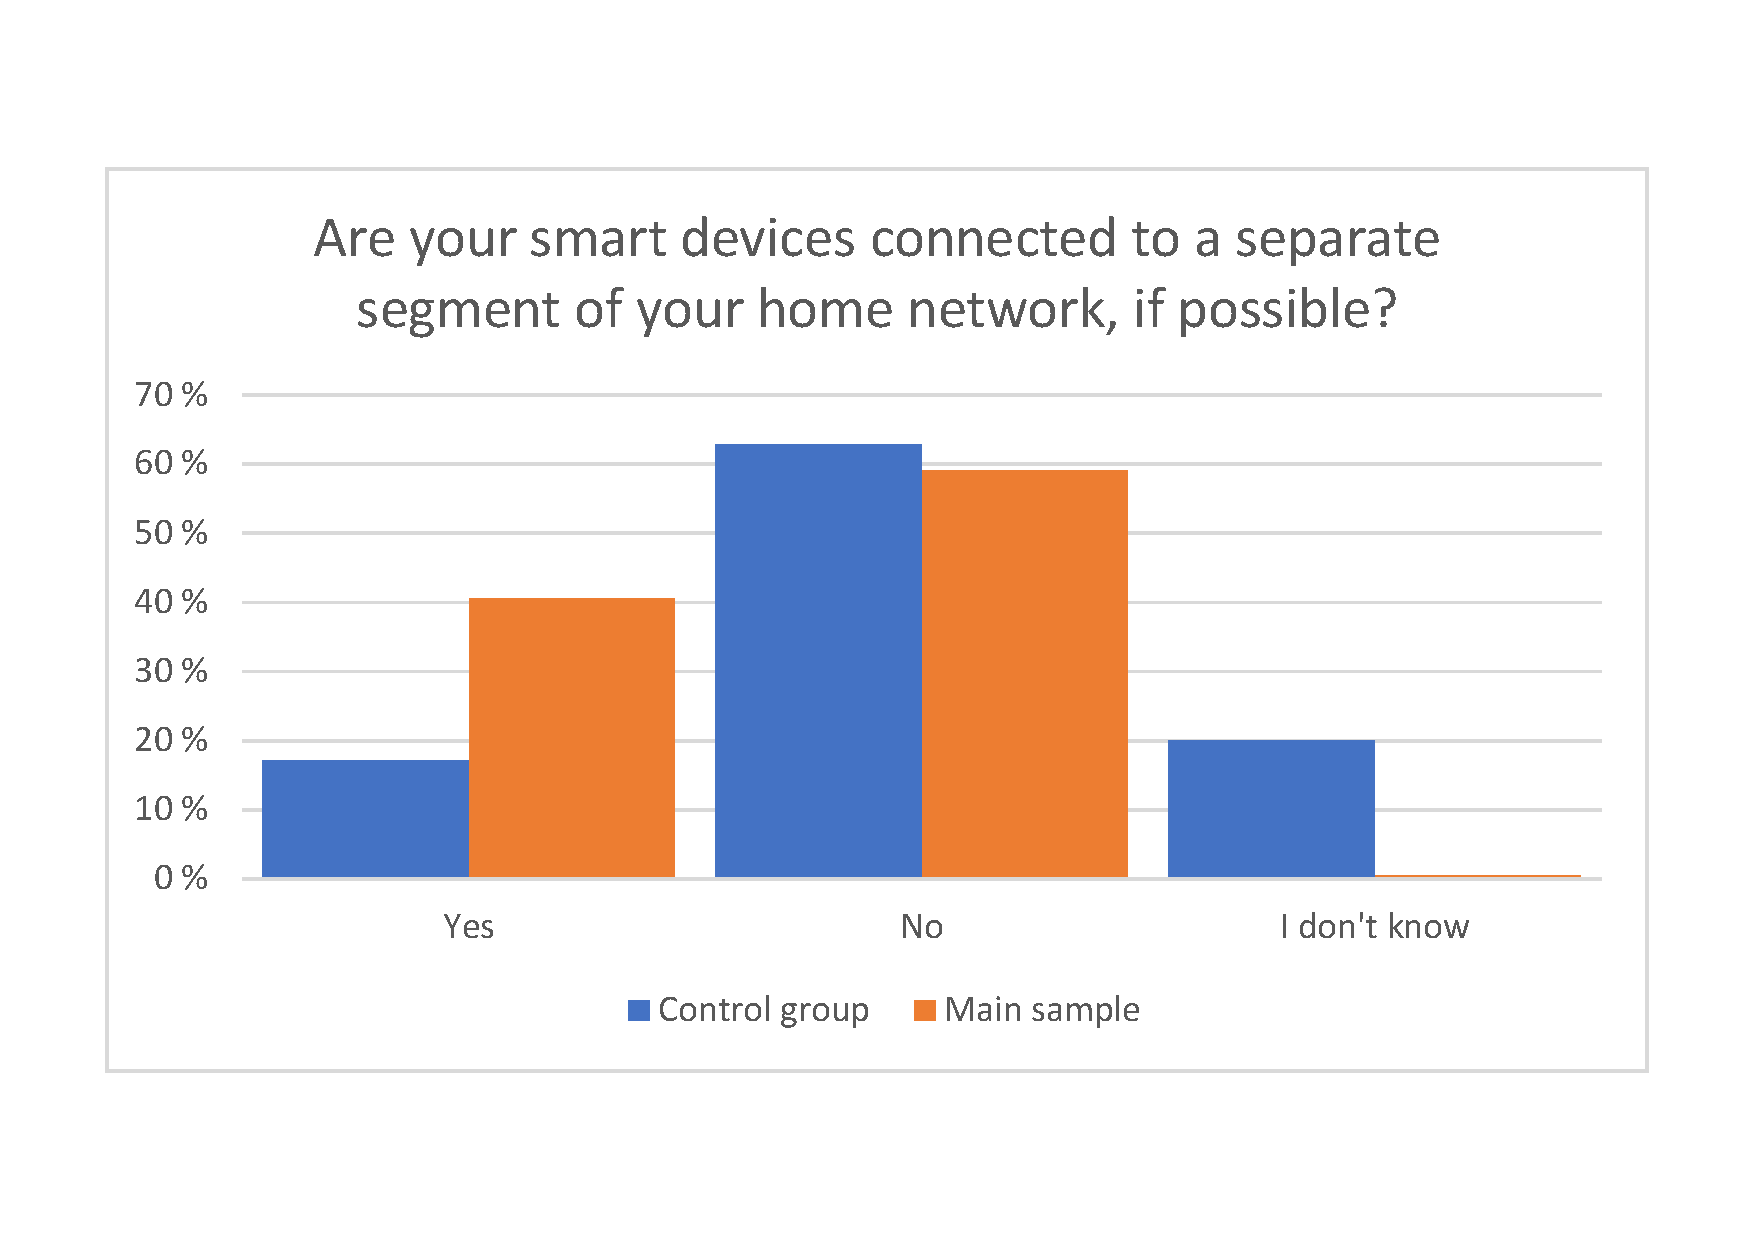
\includegraphics[scale=0.40]{figures/diagrams/controlgroup_separatesegment.pdf}
    \caption{Differences between the samples in usage of a separate segment of the home network for smart devices}
    \label{fig:controlgroup_separatesegment}
\end{figure}

I also found an interesting difference between the samples when it comes to preference towards using wireless or cable to connect to the internet. For the control group sample, 10 people (28.6\%) answered that they preferred cable where possible, to the 64\% of the main sample. On the other hand, 23 people (65.7\%) from the control group preferred wireless, compared to the 21\% of the main sample group. The results are visualised in figure \ref{fig:controlgroup_cablewireless}. 
\begin{figure}[!h]
    \centering
    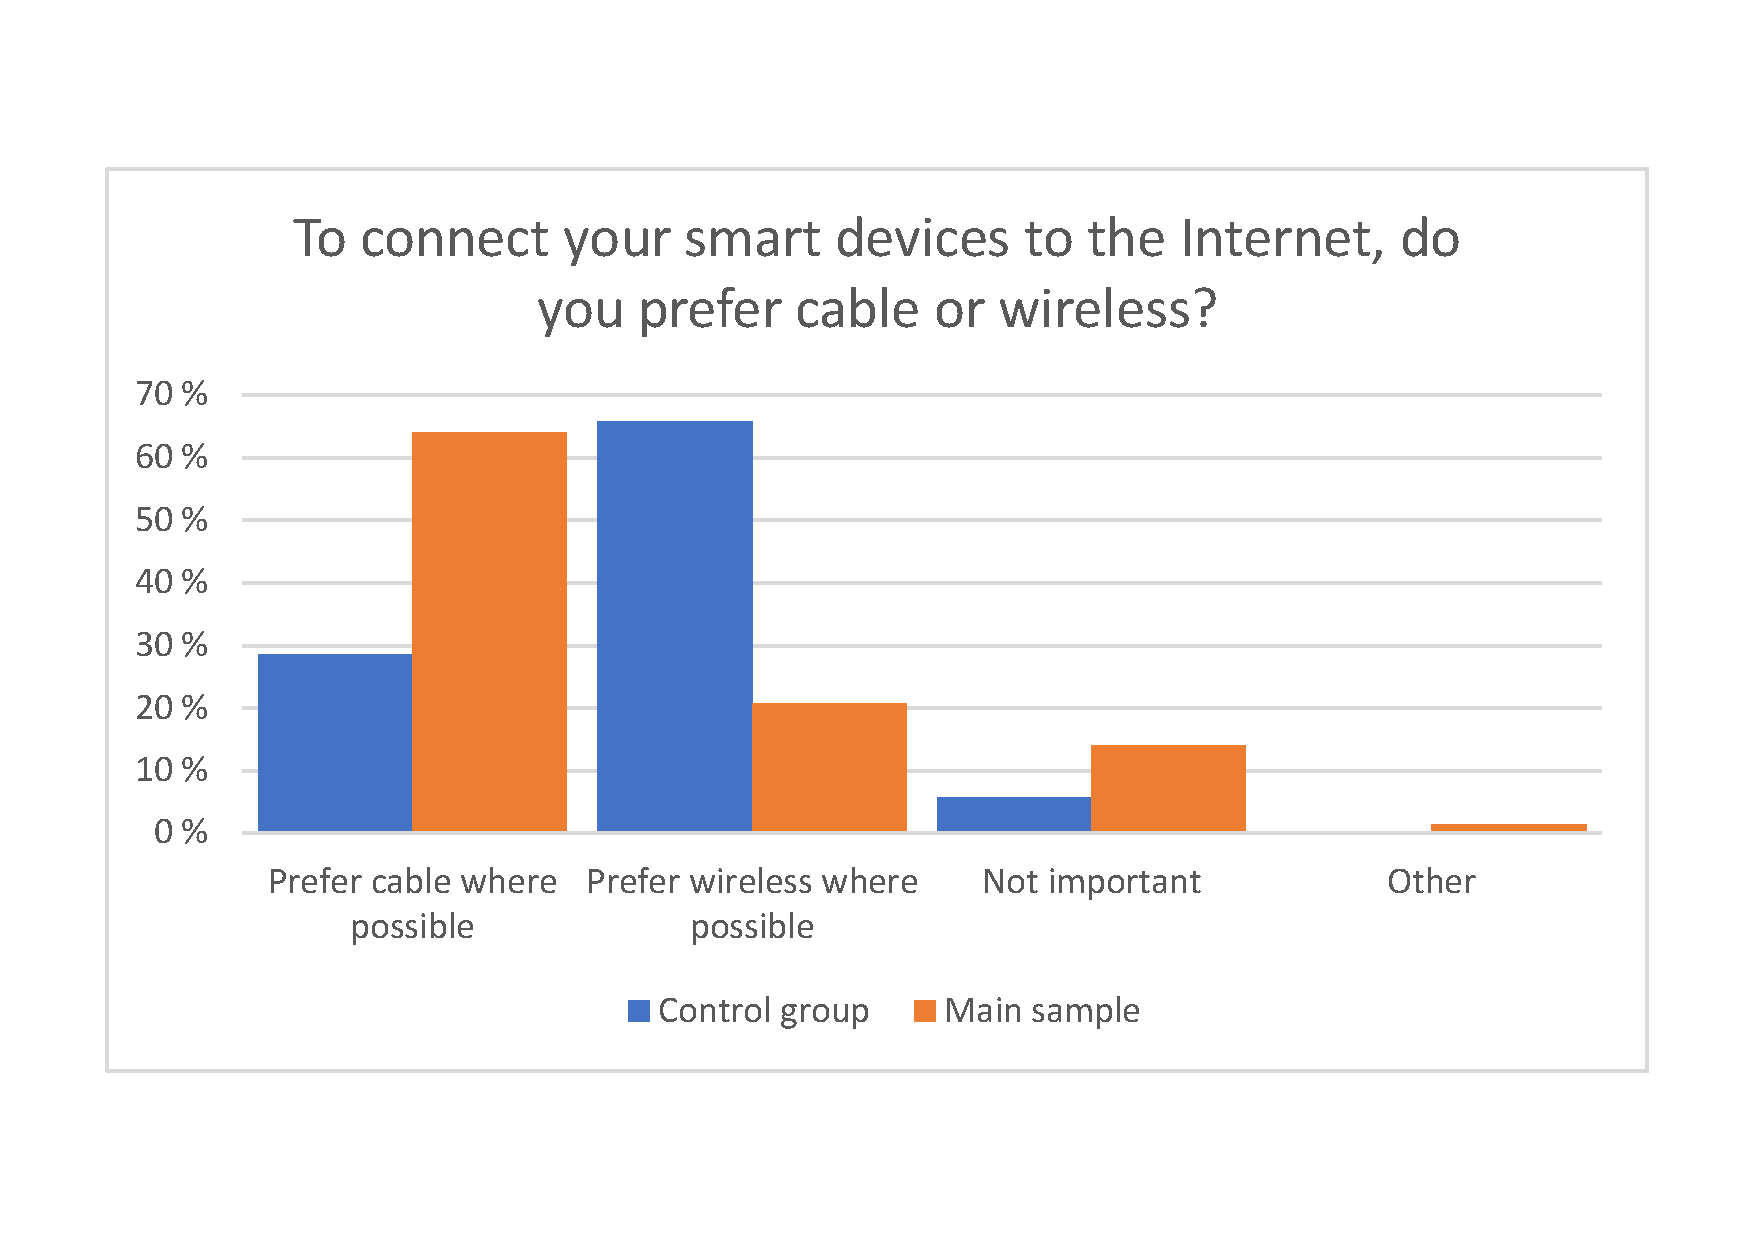
\includegraphics[scale=0.40]{figures/diagrams/controlgroup_cablewireless.pdf}
    \caption{Differences between the samples in preferring cable or wireless to connect smart devices to the internet}
    \label{fig:controlgroup_cablewireless}
\end{figure}

Both these questions were answered only by people who owned smart home devices. 

\subsubsection{Differences in credential management}
Other findings in differences between the samples included a question regarding credential management. This question aimed to figure assess if the respondents used the same password on multiple devices and services. The results can be viewed in figure \ref{fig:controlgroup_samepassword} below. 
\begin{figure}[!h]
    \centering
    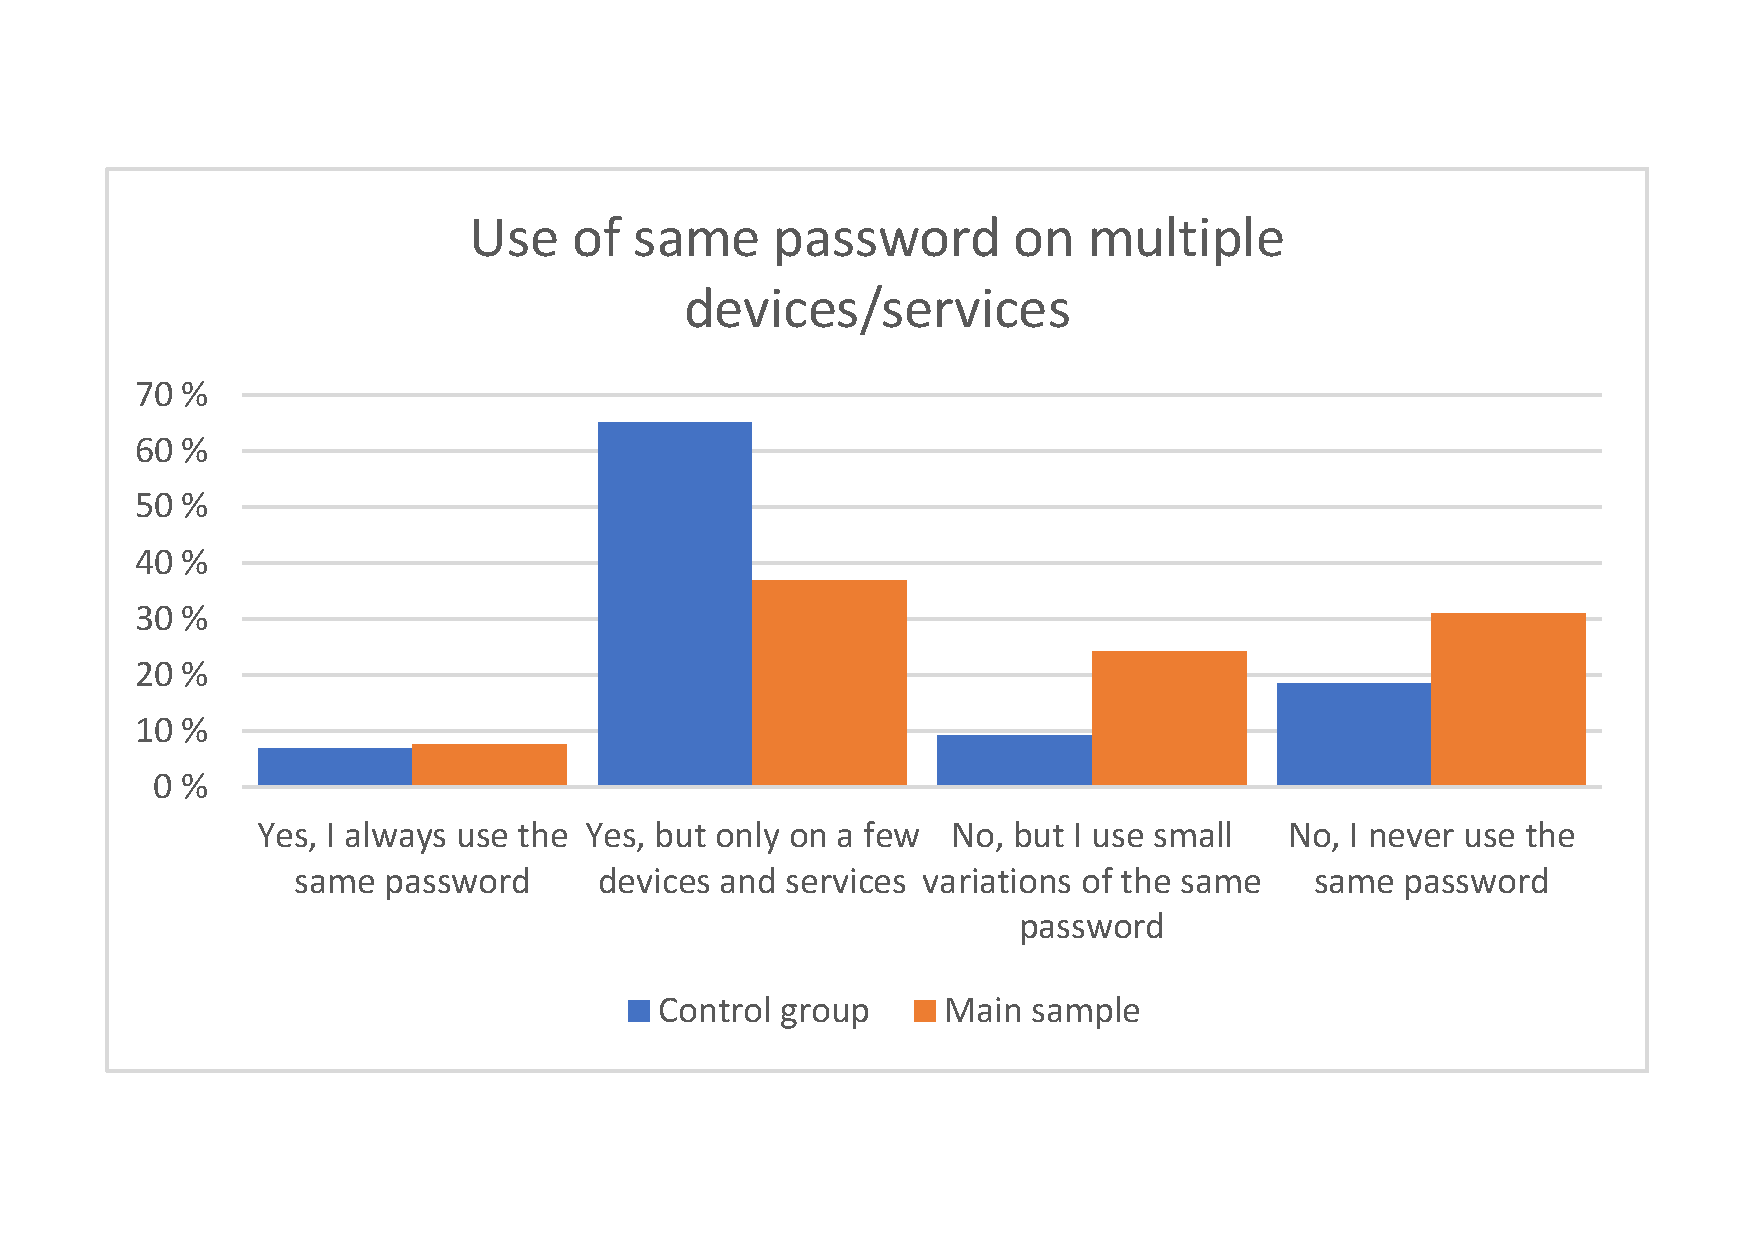
\includegraphics[scale=0.40]{figures/diagrams/controlgroup_samepassword.pdf}
    \caption{Differences between the samples in using the same password on multiple devices/services}
    \label{fig:controlgroup_samepassword}
\end{figure}
I observed that around the same amount of people used the same password, however 28 people (65\%) from the control group sample admitted to using the same password on a few services and devices, compared to the 37\% from the main sample. This also means that fewer people from the control group answered that the do not use the same password. 

\subsubsection{Differences in risk perception}
I also looked at the differences in risk perception between the samples based on the 8 risk scenarios that were analysed in section \ref{subsec:risk_perception}. Looking at the descriptive statistics I found that overall, the control group sample perceived the risk from these scenarios slightly higher than the main sample. The descriptive statistics can be viewed in table \ref{tab:controlgroup_riskperception_desc} in the appendix. 